\documentclass{article}
\usepackage[T2A]{fontenc}
\usepackage[utf8]{inputenc}
\usepackage{enumitem}
\usepackage{wrapfig}
\usepackage{tabularx}
\usepackage{listings}
\usepackage[yyyymmdd]{datetime}

\usepackage{pgfplots} %For rainbow sinewave plot along right side.
% \usepgfplotslibrary{external}
% \tikzexternalize
\pgfplotsset{compat=1.14}

\DeclareMathAlphabet{\mathrm}{OT1}{cmss}{m}{n}

%Fix up for poorly hyphenated words.
\hyphenation{meas-ured Micro-wave}

\usepackage{url}

% Actual poster will be 20x39"
% artwork will be 1 inch larger 21x40
\usepackage[textwidth=\textwidth,textheight=\textheight]{geometry}
%Actual paper size is 20x39
%Full bleed oversize by 0.5in on each side. 21x40
\geometry{
	verbose,
	noheadfoot,
	paperwidth=21in,
	paperheight=40in,
	top=0in,
	bottom=0in,
	left=0in,
	right=0in
}

\usepackage{pstricks,pst-poly,pst-3d,pst-node,pst-tree,pst-grad,pst-plot,pst-3dplot,pst-solides3d}

% \usepackage[pstricks,squaren,cdot]{SIunits}	% used for SI units and other symbols like mu
\usepackage{siunitx}	% used for SI units and other symbols like mu



\newfont{\titlefont}{cmssbx10 at 50pt}    %Title Font

\usepackage{color}
\usepackage{calc}
\usepackage{multido}
\usepackage{graphicx} %for the includegraphics function

%Allow polar co-ordinates (radius,angle) with pstricks
\SpecialCoor

\definecolor{Black}{rgb}{0.0,0.0,0.0} %Printer uses this layer as CMYK. For testing, alter the values from 0,0,0.
  
\pagecolor{Black}
\pagestyle{empty}	% suppress page numbering

%Some backgrounds must be same black as gradient, cannot use CMYK black.
%Try this trick to make an RGB black for the printhouse, use a black that is not quite black.
\definecolor{RGBBlackBegin}{rgb}{0.001,0.001,0.001}
\definecolor{RGBBlackEnd}{rgb}{0.002,0.002,0.002}

\definecolor{IonizingYellow}{rgb}{.88,.88,0}
\definecolor{Itinerant}{rgb}{0.5,1.0,0.5} %Itinerant frequency color


\definecolor{Brown}{rgb}{0.65,0.16,0.16}
\definecolor{DarkBrown}{rgb}{0.463,0.141,0}
\definecolor{BrightGreen}{rgb}{0.5,1,.5}
\definecolor{LineGray}{rgb}{0.6,0.6,0.6}
\definecolor{Gray80}{rgb}{0.8,0.8,0.8}
\definecolor{Gray20}{rgb}{0.2,0.2,0.2}

\definecolor{FColor}{rgb}{0.8,0.8,1.0} %Frequency label color
\definecolor{WColor}{rgb}{0.8,1.0,0.8} %Wavelength label color
\definecolor{EColor}{rgb}{1.0,0.8,0.8} %Energy label color

\definecolor{DarkRange}{rgb}{0.2,0.2,0.2}
\definecolor{LightRange}{rgb}{0.3,0.3,0.3}

\newlength{\VerticalSeparation}  \setlength{\VerticalSeparation}{.1in} %vertical separation of text boxes

\newlength{\EMRPosition}  \setlength{\EMRPosition}{-.85in} %vertical centerline for arrows
\newlength{\EMRPositionA} \setlength{\EMRPositionA}{\EMRPosition-0.2in}
\newlength{\EMRPositionB} \setlength{\EMRPositionB}{\EMRPosition+0.1in}
\newlength{\EMRPositionC} \setlength{\EMRPositionC}{\EMRPosition-0.37in} %Far left side of box
\newlength{\EMRPositionD} \setlength{\EMRPositionD}{\EMRPosition+0.27in} %vertical centerline for alternative arrows
\newlength{\EMRPositionE} \setlength{\EMRPositionE}{10.1in} %far right side grey backgrounds on chart

\newlength{\AudioPosition}    \setlength{\AudioPosition}{10.4in} % xpos centerline
%\newlength{\AudioPositionA}   \setlength{\AudioPositionA}{\AudioPosition-0.1in} %label left side
\newlength{\AudioPositionA}   \setlength{\AudioPositionA}{\AudioPosition} %label left side
\newlength{\AudioPositionB}   \setlength{\AudioPositionB}{\AudioPosition+0.1in} %label right side
% \newlength{\AudioPositionC}   \setlength{\AudioPositionC}{\AudioPosition-0.2in} %display box left side
\newlength{\AudioPositionC}   \setlength{\AudioPositionC}{\AudioPosition-0.1in} %display box left side
\newlength{\AudioPositionD}   \setlength{\AudioPositionD}{\AudioPosition+0.5in} %display box right side
\newlength{\AudioPositionE}   \setlength{\AudioPositionE}{\AudioPosition+0.1in} %right side of piano keys
\newlength{\AudioPositionF}   \setlength{\AudioPositionF}{\AudioPosition-0.5pt} %left side of centerline
\newlength{\AudioPositionG}   \setlength{\AudioPositionG}{\AudioPosition+0.5pt} %right side of centerline
\newlength{\AudioPositionH}   \setlength{\AudioPositionH}{\AudioPosition+0.2in} % approx center for some minipage labelling.


% set normal size text for math fonts
\newcommand{\D}{\displaystyle}

% remove all itemize left margins for compactness.
\setlist[itemize]{leftmargin=*}

% Erbium-Doped Fiber Amplifier
% \edfa{center Xpos, bottom Ypos}
  \newcommand{\fiberoptics}[2]{
  \rput(#1){
	\psset{fillstyle=solid,fillcolor=yellow,framesep=2pt,linearc=0,linestyle=none}
	%\psframe[fillstyle=solid,fillcolor=yellow](-.175,.05)(.175,.25)
	\psline[fillstyle=none,linestyle=solid,linewidth=1.5pt,linecolor=yellow](-.17,0)(-.17,.2)(.17,.2)(.17,0)
	\rput(0,.15){\psframebox[fillstyle=solid,framesep=1pt]{\textcolor{Black}{#2}}}
  }}


  %draw a tiny submarine{location}{text}
  % The submarine was drawn using xfig then exported as an "Latex picture + epic macros" then the co-ordinates copied into here below
  \newcommand{\submarine}[2]{
  	\rput(#1){\rput(-.27,-.07){
	\psline[unit=.0006in,linecolor=green,fillstyle=solid,fillcolor=WColor,linestyle=solid,linearc=0]{-}(29,190)(240,217)(268,336)
        (403,315)(414,217)(718,201)
        (957,163)(989,244)(1016,250)
        (1016,158)(1027,152)(1027,104)
        (1016,98)(1016,12)(984,17)
        (957,104)(729,50)(528,28)
        (154,28)(40,55)(18,82)
        (12,158)(29,190)}}
	\rput(#1){\textcolor{Black}{#2}}}

  \newcommand{\timestandard}{\psset{linecolor=Black,linewidth=1pt,linearc=0}
	\psframebox[linestyle=none]{%
		\pscircle[linestyle=none,fillstyle=solid,fillcolor=white]{.11}
		\pscircle[fillstyle=none,linestyle=solid]{.1}
		\psline[fillstyle=none,linestyle=solid]{c-c}(.07;150)(0;0)(.05;30)
		\psline[linestyle=solid](.07;0)(.1;0)
		\psline[linestyle=solid](.07;90)(.1;90)
		\psline[linestyle=solid](.07;180)(.1;180)
		\psline[linestyle=solid](.07;270)(.1;270)
		}
	}

  \newcommand{\weatherstation}{
	\psset{linecolor=white,linewidth=1pt,linestyle=solid,fillstyle=solid,fillcolor=white,linearc=0}
	\psframebox[linestyle=none,fillstyle=none]{
		\pscircle(-.03,0.03){.05}
		\pscircle(0.03,0.03){.05}
		\pscircle(-.03,-.03){.05}
		\pscircle(0.03,-.03){.05}
		\psline(-.12,.05)(0.0,.05)
		\psline(-.11,.02)(0.01,.02)
		\psline(-.10,-.01)(0.02,-.01)
		\rput(0,0){\black W}
		}
  }

  \newcommand{\pager}{
	\psset{linecolor=green,linewidth=0.7pt,linestyle=solid,fillstyle=solid,fillcolor=red,linearc=0}
	\psframebox[linestyle=none,fillstyle=none]{
		\psline(0,0)(0,-.1)
		\pscircle(0,0){.05}
		\rput(0,0){\tiny\black P}
	}
  }


  \newcommand{\wirelessmic}{
	\psset{linecolor=Gray20,linewidth=0.7pt,linestyle=solid,fillstyle=solid,fillcolor=DarkBrown,linearc=0}
	\psframebox[linestyle=none,fillstyle=none]{
		\pscurve[linearc=0.04,linewidth=0.5pt,fillstyle=none](-0.015,0.06)(0,0.07)(0,0.09)(0,0.12)
		\psline[linewidth=1.8pt](0,0.1)(0,0.2)
		\pscircle(0,0.2){.03}
	}
  }


  \newcommand{\astrofilter}[2]{
	\rput(#1){\black\bfseries%\tiny
		%\psline[fillstyle=solid,fillcolor=white,linestyle=none](.10;90)(.10;234)(.10;18)(.10;162)(.10;306)(.10;90)
		%\rput(0,0){\pscircle[fillstyle=solid,fillcolor=white,linestyle=none](0,0){.1}}
		%\rput(0,0){#2}
		%\rput(0,0){\psdots[linecolor=white](.15;0)(.15;40)(.15;80)(.15;120)(.15;160)(.15;200)(.15;240)(.15;280)(.15;320)}
		\psline[linecolor=white,linestyle=solid,linewidth=1pt](-.1,-.07)(-.1,.07)
		\psline[linecolor=white,linestyle=solid,linewidth=1pt](.1,-.07)(.1,.07)
		\psframe[fillcolor=white,fillstyle=solid,linestyle=none](-.1,-.05)(.1,.05)
		\rput(0,0){#2}
	}
  }

  \newcommand{\blip}[2]{
	\rput(#1){
% 		\pscurve[linestyle=solid,linewidth=.8pt,linecolor=black,fillstyle=solid,fillcolor=white](-.1,0)(-.08,.02)(0,.2)(.08,.02)(.1,0)
		\pscurve[linestyle=solid,linewidth=.8pt,linecolor=black,fillstyle=solid,fillcolor=white](-.1,0)(-.08,.05)(0,.25)(.08,.05)(.1,0)
		\psline[linestyle=solid,linewidth=.8pt,linecolor=white](-.12,0)(.12,0)
		\rput(0,0.15){\textcolor{Black}{#2}}
	}

  }

%%%%%%%%%%%%%%%%%%%%%%%%%%%%%%%%%%%%%%%%%%%%%%%%%%%%%%%%%%%%%%%%%%%%%%%%%%%%%%%%%%%%%
% Notes:
%  - Calibration of the paper size is done with the "\psset{unit=Xin}" setting below
%    where X should be close to 1.000 depending on your printer.
%  - All rows are spaced 0.5" apart.
%  - All columns are determined by dividing the desired width by 12.
%  - The width should be determined by measuring the circumference of the tube that
%    the chart is to be wrapped around.
%    Measure this accurately or use trial and error to line up the sheet once wrapped
%    around cylinder.
%%%%%%%%%%%%%%%%%%%%%%%%%%%%%%%%%%%%%%%%%%%%%%%%%%%%%%%%%%%%%%%%%%%%%%%%%%%%%%%%%%%%%

\begin{document} %===================================================================
\flushleft%
%
%\tiny
%\scriptsize
%\footnotesize
\small%
%\normalsize
%\large
%\Large
%\LARGE
%\huge
%\Huge
%
\sffamily%
%
\psset{unit=1in}% scaling factor for perfect printer to equal 1.000"
%
\begin{pspicture}(-.49,-.49)(20.49,39.49)% Dimensions must include all printable objects inside otherwise auto-pst-pdf will crop out items. Also, auto-pst-pdf adds 0.01in to width and height, compensate by subtracting that from the desired dimension -0.005 on each side and again since fitting this picture into the paper seems to require a bit of space also.
%
	\newlength{\nLeftWidth}\setlength{\nLeftWidth}{6.24in}
	\rput(12.7,26.36){
{
  %Upper Left side notes
  
  \psset{cornersize=absolute,linearc=4pt,fillstyle=solid,fillcolor=Black, linecolor=white}
  \white

  \rput[bl]{0}(0,0){
    \parbox[t]{\nLeftWidth}{

	\psframebox{\parbox[t]{\nLeftWidth}{\white{
\psset{linearc=0}
{\Large How to read this chart}
\begin{itemize}

\item This chart is organized in octaves (frequency doubling/halving) starting at 1Hz and going higher (2,4,8, etc) and lower (1/2, 1/4, etc). The octave is a natural way to represent frequency.

\item Frequency increases in the upward direction. and wrap around from far right to far left.

%\item This chart was also designed so that the spectrum section could be cut our and wrapped around a standard 3 inch diameter by 36 inches long mailing tube to represent a continuous frequency from the bottom to the top and beyond.

\item There is no limit to either end of this chart, however, due to limited space, only the ``known" items have been shown here. A frequency of 0Hz is the lowest possible frequency but the method of depicting octaves used here does not allow for ever reaching 0Hz, only approaching it. Also, by the definition of frequency (Cycles per second), there is no such thing as negative frequency.

\item Values labels: \psframebox[framesep=1pt,fillstyle=solid,fillcolor=Black]{\textcolor{FColor}{Frequency}} in Hertz,%
\psframebox[framesep=1pt,fillstyle=solid,fillcolor=Black]{\textcolor{WColor}{Wavelength}} in meters,%
\psframebox[framesep=1pt,fillstyle=solid,fillcolor=Black]{\textcolor{EColor}{Energy}} in electronVolts.

\end{itemize}
}
}}

	\vspace{\VerticalSeparation}
	
	\psframebox{\parbox[t]{\nLeftWidth}{\white\input{tex/gammarays.tex}}}

	\vspace{\VerticalSeparation}


	\psframebox{\parbox[t]{\nLeftWidth}{{\Large {\bfseries U}ltra{\bfseries v}iolet Light ({\bfseries UV})}
\begin{itemize}
\item UV light is beyond the range of human vision. A bumblebee can see light in the UVA range which helps them identify certain flowers.

% \item Physicists have divided ultraviolet light ranges into Vacuum Ultraviolet (VUV), Extreme Ultraviolet (EUV), Far Ultraviolet (FUV), Medium Ultraviolet (MUV), and Near Ultraviolet (NUV).

% \item UV-A, UV-B and UV-C were introduced in the 1930's by the Commission Internationale de l'\'{E}clairage (CIE, International Commission on Illumination) for photobiological spectral bands.

\item Short-term UV-A exposure causes sun-tanning which helps to protect against sunburn. Exposure to UV-B is beneficial to humans by helping the skin produce vitamin D. Excessive UV exposure causes skin damage. UV-C is harmful to humans but is used as a germicide.

% \item The CIE originally divided UVA and UVB at 315nm, later some photo-dermatologists divided it at 320nm.

% \item UVA is subdivided into UVA1 and UVA2 for DNA altering effects at 340nm.

\item The Sun produces a wide range of wavelengths including all the UV light, however, UVB is partially filtered by the ozone layer and UVC is totally filtered out by the earth's atmosphere.

\end{itemize}




% From: http://www.ping.at/cie/publ/abst/134-99.html
% Press Release:
% CIE Collection in Photobiology and Photochemistry, 1999
% CIE 134-1999 ISBN 3 900 734 94 1
% This volume contains short Technical Reports prepared by various Technical Committees within CIE Division 6.

% 134/1: TC 6-26 report: Standardization of the Terms UV-A1, UV-A2 and UV-B
% The terms UV-A, UV-B and UV-C were introduced in the 1930's by CIE Committee 41 on Ultraviolet Radiation as a short-hand notation for photobiological spectral bands. It was never intended that the bands were exclusive for different effects. The bands have been in widespread use in different medical fields and scientific research. UV-A and UV-B were divided at 315 nm by the CIE. In recent decades, some photo-dermatologists and others have used different dividing lines such as 320 nm without recognizing the importance of maintaining an international standardized terminology. Because the terminology is used in many fields, this report recommends that the 315 nm division between UV-A and UV-B be maintained. However, recent research has clearly shown a difference in the photobiological interaction of long and short wavelength UV-A radiation with DNA. This led to a further division of UV-A into UV-A1 and UV-A2 with a dividing line at approximately 340 nm. While this division may be of value, the committee does not recommend officially to split UV-A into these two sub-bands at this time. Further research may justify a dividing line different from 340 nm in the future.
}}

	\vspace{\VerticalSeparation}

	\psframebox{\parbox[t]{\nLeftWidth}{%Emission and Absorption lines
{\Large Emission and Absorption}
\begin{itemize}

%\item The fluorescent lamp uses luminescent material (phosphor) to convert ultraviolet radiation using photoluminescence into visible light. The phosphor absorbs UV light and emits visible light.

\item As EMR passes through elements, certain wavelength bands get absorbed and some new ones get emitted. This absorption and emission produces characteristic spectral lines for each element which are useful in determining the makeup of distant stars. These lines are used to prove the red-shift amount of distant stars.

\item
 When a photon hits an atom it may be absorbed if the energy is just right.
 The energy level of the electron is raised -- essentially holding the radiation.
 A new photon of specific wavelength is created when the energy is released.
 The jump in energy is a discrete step and many possible discrete levels of energy exist in an atom.

\item \begin{minipage}[t]{3.5in} Johann Balmer created this formula defining the photon emission wavelength ($\lambda$); where $m$ is the initial electron energy level integer number and $n$ is the final electron energy level integer number: \end{minipage}%
\hspace{0.2in}
\begin{minipage}[t]{1.5in}\vspace{0.01in}
	$\lambda = 364.56nm \left( \frac{\D m^2}{\D m^2 - n^2} \right)$
\end{minipage}

\vspace{0.02in}

\item Much of the interstellar matter is made of the simplest atom hydrogen. The hydrogen visible-spectrum emission and absorption lines are shown below:

\end{itemize}

%what happens if the photons energy is slightly higher than required to elevate the electrons energy level? Where does the excess energy go after raising the electrons energy level?


%Start X, End X, Label, label offset
\newcommand{\absorbemit}[4]{
	\psframe(#1,.075)(#2,.165)
	\psline[linestyle=solid](#2,0)(#2,.083)
	\uput{2pt}[270](#2,#4){#3}
}
\vspace{0.15in}
\psframebox[fillstyle=none,linestyle=none]{
	\rput(0.1,0){
	%Start at 760nm (0in)
		\psset{
			xunit=.0156in, % Change for length.
			linestyle=none, 
			linewidth=1pt, 
			linecolor=Black, 
			fillstyle=solid, 
			fillcolor=Black,
			linearc=0
		}
{
%  Red 		760-620 nm
%  Orange 	620-570 nm
%  Yellow 	570-550 nm
%  Green 	550-470 nm
%  Blue 	470-440 nm
%  Violet 	440-380 nm
\psset{gradlines=100,fillstyle=gradient,gradangle=90,gradmidpoint=1.0,linewidth=0pt,linestyle=none}
\definecolor{StartColor}{hsb}{.0,1,1} \definecolor{EndColor}{hsb}{.1,1,1} \psframe[gradbegin=StartColor,gradend=EndColor](0,0)(165,.15) %Red to Orange
\definecolor{StartColor}{hsb}{.1,1,1} \definecolor{EndColor}{hsb}{.2,1,1} \psframe[gradbegin=StartColor,gradend=EndColor](165,0)(200,.15) %Orange to Yellow
\definecolor{StartColor}{hsb}{.2,1,1} \definecolor{EndColor}{hsb}{.38,1,1}\psframe[gradbegin=StartColor,gradend=EndColor](200,0)(250,.15) %Yellow to Green
\definecolor{StartColor}{hsb}{.4,1,1} \definecolor{EndColor}{hsb}{.5,1,1} \psframe[gradbegin=StartColor,gradend=EndColor](250,0)(305,.15) %Green to Blue
\definecolor{StartColor}{hsb}{.5,1,1} \definecolor{EndColor}{hsb}{.8,1,1} \psframe[gradbegin=StartColor,gradend=EndColor](305,0)(380.25,.15) %Blue to Violet
}
		\absorbemit{-2}{103.715}{$H_\alpha$}{0}
		\absorbemit{103.715}{273.867}{$H_\beta$}{0}
		\absorbemit{273.867}{325.953}{$H_\gamma$}{0}
		\absorbemit{325.953}{349.826}{$H_\delta$}{0}
		\absorbemit{349.826}{363.03}{$H_\epsilon$}{0}
		\absorbemit{363.03}{371.14}{$H_\zeta$}{-.13in}
		\absorbemit{371.14}{376.5}{$H_\eta$}{.32in}
		\absorbemit{376.5}{380.25}{$H_\theta$}{0}
		\absorbemit{380.25}{385}{}{0}
{
	\psset{linearc=2pt,linecolor=white,linestyle=solid,linewidth=1pt,fillstyle=none}
	\uput{2pt}[180](70,.17){Emission line}\psline{->}(70,.17)(86,.17)(86,.12)(102,.12)
	\uput{2pt}[180](70,-.10){Absorption line}\psline{->}(70,-.10)(86,-.10)(86,.04)(102,.04)
	\uput{2pt}[0](140,-.16){Balmer series name}\psline{->}(140,-.16)(127,-.16)(127,-.09)(113,-.09)
}
	}
}
\vspace{0.2in}

%longer at opposite end, must use negative co-ordinates (Ex. subtract from the beginning of red visible light 760nm )
%$H_\alpha$% 656.285nm  103.715
%$H_\beta$% 486.133nm 273.867
%$H_\gamma$% 434.047nm 325.953
%$H_\delta$% 410.174nm 349.826
%$H_\epsilon$% 396.97nm 363.03
%$H_\zeta$% 388.86nm 371.14
%$H_\eta$% 383.50nm 376.5
%$H_\theta$% 379.75nm 380.25

%from http://hyperphysics.phy-astr.gsu.edu/hbase/quantum/atspect.html#c1

%Emission
%Wavelength	Relative	Transition	Color
%(nm)		Intensity
%383.5384 	5 		9 -> 2 		Violet
%388.9049 	6 		8 -> 2 		Violet
%397.0072 	8 		7 -> 2 		Violet
%410.174 	15 		6 -> 2 		Violet
%434.047 	30 		5 -> 2 		Violet
%486.133 	80 		4 -> 2 		Bluegreen (cyan)
%656.272 	120 		3 -> 2 		Red
%656.2852 	180 		3 -> 2 		Red


\textcolor{gray}{\hrule}
\vspace{.1in}
\hspace{.1in}
\begin{tabular}{rl}
%Blackbody radiation
\begin{minipage}[t]{1.3in}
\rput(0,-.65){
	\psframebox[linestyle=none]{
		%
		%The following picture was created using the above Plank formula in a 
		% spreadsheet (balmer_series.gnumeric) then plotted.
		%The vertical scale is log(x), temperatures are 2000K, 1000K, 700K.
		\rput[bl](0,0){\includegraphics{pictures/blackbody.eps}}
		%
		%Labelling for the plot:
		\psline[fillstyle=none, linearc=0]{<->}(1.1,0)(0,0)(0,.8)
		\rput[b]{90}(-.05,.45){Power}
		\rput[t](.5,-.05){Wavelength}
		\psset{border=1pt, bordercolor=Black, fillstyle=none, linearc=0,linecolor=green}
		\psline{o-}(.08,.6)(.5,.6)\uput{2pt}[0](.5,.6){White Hot}
		\psline{o-}(.12,.43)(.7,.43)\uput{2pt}[0](.7,.43){Red Hot}
		\psline{o-}(.18,.25)(.9,.25)\uput{2pt}[0](.9,.25){Hot}
		\psline{o-}(.7,0)(.88,.1)(1.05,.1)\uput{2pt}[0](1.05,.1){CMB}
	}
}
\end{minipage}&
\begin{minipage}[t]{2.4in}
	\begin{itemize}
		\item Max Planck determined the relationship between the temperature of an object and its radiation profile; where $R_\lambda$ is the radiation power, $\lambda$ is the wavelength, $T$ is the temperature:
	\end{itemize}
\end{minipage}
\begin{minipage}[b]{2.5in}
	\rput(.9in,-.3in){$R_\lambda = \frac{\D 37418}{\D \lambda^5 \epsilon^{\left( \frac{\D 14388}{\D \lambda T}\D - 1 \right) }}$}
\end{minipage}

\end{tabular}
\vspace{.15in}

% Atmospheric electromagnetic transmittance or opacity.jpg
% https://commons.wikimedia.org/wiki/File:Atmospheric_electromagnetic_transmittance_or_opacity.jpg
% This file is in the public domain in the United States because it was solely created by NASA. NASA copyright policy states that "NASA material is not protected by copyright unless noted". (See Template:PD-USGov, NASA copyright policy page or JPL Image Use Policy.)	
% 	Warnings:
% Use of NASA logos, insignia and emblems is restricted per U.S. law 14 CFR 1221.
% The NASA website hosts a large number of images from the Soviet/Russian space agency, and other non-American space agencies. These are not necessarily in the public domain.
% Materials based on Hubble Space Telescope data may be copyrighted if they are not explicitly produced by the STScI.[1] See also {{PD-Hubble}} and {{Cc-Hubble}}.
% The SOHO (ESA & NASA) joint project implies that all materials created by its probe are copyrighted and require permission for commercial non-educational use. [2]
% Images featured on the Astronomy Picture of the Day (APOD) web site may be copyrighted. [3]
% The National Space Science Data Center (NSSDC) site has been known to host copyrighted content. Its photo gallery FAQ states that all of the images in the photo gallery are in the public domain "Unless otherwise noted."







%Fluorescent lamp 12,000K
%Sun 6,000K
%Incandescent lamp 3000K
%Cosmic Microwave Background radiation 3K

}}

	\vspace{\VerticalSeparation}

	\psframebox{\parbox[t]{\nLeftWidth}{\white{
% \newcommand{\nVSLength}{0.170}
% \newcommand{\nVSEnd}{0.171}%slightly larger 0.001 than increment length to prevent breaking of chunks on PDF viewer.

\newlength{\nVSLength}	\setlength{\nVSLength}{0.56in}
\newlength{\nVSEnd}	\setlength{\nVSEnd}{0.001in+\nVSLength}
\newlength{\nRightSide}	\setlength{\nRightSide}{0in}
\newlength{\nLeftSide}	\setlength{\nLeftSide}{0in}

\psset{gradlines=100,
 fillstyle=gradient,
 gradangle=90,
 gradmidpoint=1.0,
 linewidth=0pt,
 linestyle=none,
 linearc=0pt}
{\Large Visible Spectrum \hspace{0.07in}
	\psframebox[fillstyle=none,linestyle=none]{%
		\psset{xunit=2.8in}
		\multido{%
			\nCounter=0+1,
			\nStartColor=0.00+0.1,
			\nEndColor=0.1+0.1
			}{8}{%
			\setlength{\nRightSide}{\nVSEnd+\nVSLength*\nCounter}
			\setlength{\nLeftSide}{\nVSLength*\nCounter}
			\definecolor{StartColor}{hsb}{\nStartColor,1,1}
			\definecolor{EndColor}{hsb}{\nEndColor,1,1}
			\psframe[fillstyle=gradient,
				gradangle=90,
				gradbegin=StartColor,
				gradend=EndColor,
				gradmidpoint=1.0,
				linewidth=0pt,
				linestyle=none]
			(\nLeftSide,0in)(\nRightSide,0.15in)
		}
	}
}
\begin{itemize}

\item The range of EMR visible to humans is called ``Light". The visible spectrum also closely resembles the range of EMR that filters through our atmosphere from the Sun.

\item Other creatures see different ranges of visible light; for example bumble-bees can see ultraviolet light and dogs have a different response to colors than do humans.

\item The sky is blue because our atmosphere scatters light and the shorter wavelength blue gets scattered the most. It appears that the entire sky is illuminated by a blue light but in fact that light is scattered from the Sun. The longer wavelengths like red and orange move straight through the atmosphere which makes the Sun look like a bright white ball containing all the colors of the visible spectrum.

\item Interestingly, the visible spectrum covers approximately one octave (doubling/halving of frequency).

\item Astronomers use filters to capture specific wavelengths and reject unwanted wavelengths. The major astronomical (visual) filter bands are depicted as  \psframebox[fillstyle=none,linestyle=none]{\astrofilter{0.07,0.03}{X}}

\end{itemize}
}
}}

	\vspace{\VerticalSeparation}

    }
  }
}
}
	\rput[t](12.7,24.1){
{
  %Lower Left side notes
  \psset{cornersize=absolute,linearc=4pt,fillstyle=solid,fillcolor=Black, linecolor=white}
  \white

  \rput[tl]{0}(0,0){
    \parbox[t]{\nLeftWidth}{

 	\psframebox{\parbox[t]{\nLeftWidth}{\white{
{\Large {\bfseries L}ight {\bfseries A}mplification by {\bfseries S}timulated {\bfseries E}mission of {\bfseries R}adiation {(\bfseries LASER)}}
	\rput(0.3in,0.04in){
	\psset{	linecolor=yellow,
		fillcolor=yellow,
		linewidth=0.6pt}
		\newlength{\nLASERsize}	\setlength{\nLASERsize}{0.12in}
		\newlength{\nLASERray}	\setlength{\nLASERray}{\nLASERsize}
		\newlength{\nLASERsray}	\setlength{\nLASERsray}{0.75\nLASERsize}
		\multido{\rLASER=0+30}{6}{%Large rays
			\rput{\rLASER}(0,0){\psline(-\nLASERray,0in)(\nLASERray,0in)}
		}
		\multido{\rLASER=15+30}{6}{%Small rays
			\rput{\rLASER}(0,0){\psline(-\nLASERsray,0in)(\nLASERsray,0in)}
		}
		\pscircle(0,0){0.4\nLASERsize} %Inner circle
		\rput(0,0){\psline[linewidth=0.7pt](0in,0in)(2\nLASERray,0in)}%Long line
	}
\begin{itemize}

% \item LASER is an acronym for {\bfseries L}ight {\bfseries A}mplification by {\bfseries S}timulated {\bfseries E}mission of {\bfseries R}adiation.
\item A LASER is a device that produces coherent monochromatic EMR of high intensity .
\item With proper equipment, any EMR like visible light, ultraviolet, x-rays, and gamma rays can be made to operate like a LASER. A MASER functions similarly to the LASER and is made with with microwaves and radio waves.

%\item Junk/reword: Photons can be brought together and the resultant sum of forces is seen. If the polarization and phase are the same for the photons the the resultant light appears to be amplified. Some LASERs achieve this by constantly pumping photons into a filter to get the same frequency then bouncing those filtered photons off opposing mirrors to get the phase and polarization just right. Once the light has been ``amplified" enough it will escape from one of the mirrors.

\end{itemize}
}
}}
  
 	\vspace{\VerticalSeparation}

	\psframebox{\parbox[t]{\nLeftWidth}{%TV text
{\Large {\bfseries T}ele{\bfseries v}ision ({\bfseries TV})}
{
\definecolor{HumanAudioColor}{rgb}{0.2,0.2,0.6}
\begin{itemize}

\item Terrestrial broadcast TV uses the VHF and UHF ranges (30MHz - 3GHz)  \psframebox[linestyle=none]{\rput(0.05,.05){\psframebox[fillstyle=solid,framearc=0.25,fillcolor=red]{\textcolor{white}{\tiny 05}}}}\hspace{.1in}.

\item Satellite television is transmitted in the C-band (4 - 8 GHz)
\psframebox[linestyle=none]{\rput(0.05,.05){\psframebox[fillstyle=solid,framearc=.25,fillcolor=green]{\textcolor{black}{\tiny 05}}}}\hspace{.1in} and Ku-band (12 - 18 GHz)  \psframebox[linestyle=none]{\rput(0.04,0.02){\psdots[framesep=1pt,fillcolor=BrightGreen,fillstyle=solid,dotstyle=triangle,linecolor=BrightGreen](0,0)}}\hspace{.08in} where one of many satellites is shown. To eliminate interference, the stations are broadcast in alternating polarities, for example, Ch 1 is vertical and Ch 2 is horizontal and vice versa on neighboring satellites.

%\item Each station is transmitted in its own band.
\item TV channels transmitted through cable (CATV) are shown as  \psframebox[linestyle=none]{\rput(0.05,.05){\psframebox[fillstyle=solid,framearc=0.1,fillcolor=blue]{\textcolor{white}{\tiny 05}}}}\hspace{.1in}. CATV channels starting with ``T-" are channels fed back to the cable TV station (like news feeds).
\item 
\begin{tabular}[t]{@{}l@{\hspace{0.1in}}r}
\begin{minipage}[t]{2.8in}
Air and cable analog TV stations are broadcast with the separate video, color, and audio frequency carriers grouped together in a channel band as follows:
\end{minipage}&
\begin{minipage}[t]{2.4in}
	\rput(0,-.17in){
	\psframebox[linestyle=none]{\psset{xunit=1.25in}%was 1.7
		\psline{|<->|}(0,.28)(2.5,.28)\uput{1pt}[90](1.25,.28){6MHz}
		\white
		\psframe[linestyle=solid,framearc=0.25,fillcolor=red,fillstyle=solid](0,0)(2.5,.25)
		\psdots[linecolor=white,dotstyle=triangle*](0.625,0.02)(1.915,0.02)(2.375,0.02)
		\psline[linecolor=white](0.625,0)(0.625,.25)
		\psline[linecolor=white](1.915,0)(1.915,.15)
		\psline[linecolor=white](2.375,0)(2.375,.25)
		\psline[linecolor=white]{<->}(0,.125)(.625,.125)\rput(.29,.125){
			\psframebox[linearc=1pt,linestyle=none,framesep=0pt,fillcolor=white,fillstyle=solid]{\textcolor{Black}{1.25MHz}}}
		\psline[linecolor=white]{<->}(.625,.07)(1.915,.07)\rput(1.27,.07){
			\psframebox[linearc=1pt,linestyle=none,framesep=0pt,fillcolor=white,fillstyle=solid]{\textcolor{Black}{3.58MHz}}}
		\psline[linecolor=white]{<->}(.625,.18)(2.375,.18)\rput(1.50,.18){
			\psframebox[linearc=1pt,linestyle=none,framesep=0pt,fillcolor=white,fillstyle=solid]{\textcolor{Black}{4.5MHz}}}
		\uput{1pt}[270](.625,0){Video}
		\uput{1pt}[270](1.915,0){Color}
		\uput{1pt}[270](2.375,0){Audio}
		}
	}
\end{minipage}
\end{tabular}
%TV horizontal refresh
\item The 15.7 kHz horizontal sweep signal is a common contaminant to VLF listening \hspace{.05in}
  \psframebox[framearc=0,linearc=0]{\rput(0,.05){
	\psframe[cornersize=relative,linecolor=white, linestyle=solid, linewidth=0.8pt,fillstyle=solid,framearc=.25,fillcolor=red,linearc=0.25](-.1,-.1)(.1,.1)
	\psline[linecolor=white,linestyle=solid,linewidth=1pt]{<->}(-.1,0)(.1,0)
  }}\hspace{0.07in}.
\item Digital compression methods are used for HDTV broadcasts in order to pack more channels into the same 6MHz bandwidth as analog TV.

\end{itemize}

}



}}

	\vspace{\VerticalSeparation}

	\psframebox{\parbox[t]{\nLeftWidth}{%Radio description
{\Large Radio Bands}
%Draw a sinewave with
%	{Initial Amplitude x.xxx}{Initial Time-width x.xxx}{Initial Number of cycles x}
%	{Second Amplitude x.xxx}{Second Time-width x.xxx}{Second Number of cycles x}
%	{Total repeats}
\newlength{\nAmplitude}		\newlength{\nAmplitudeNeg}
\newlength{\nTime}		\newlength{\nTimeTwo}		\newlength{\nTimeThree}		\newlength{\nTimeFour}
\newlength{\nSAmplitude}	\newlength{\nSAmplitudeNeg}
\newlength{\nSTime}		\newlength{\nSTimeTwo}		\newlength{\nSTimeThree}	\newlength{\nSTimeFour}
\newlength{\nTimeEnd}		\newlength{\nSTimeEnd}		\newlength{\nSTimeStart}
\newcommand{\sinewave}[7]{
	\setlength{\nAmplitude}{#1}
	\setlength{\nAmplitudeNeg}{\nAmplitude*-1}
	\setlength{\nTime}{#2}
	\setlength{\nTimeTwo}{\nTime*2}
	\setlength{\nTimeThree}{\nTime*3}
	\setlength{\nTimeFour}{\nTime*4}
	\setlength{\nTimeEnd}{\nTime*4*#3}
	\setlength{\nSAmplitude}{#4}
	\setlength{\nSAmplitudeNeg}{\nSAmplitude*-1}
	\setlength{\nSTime}{#5}
	\setlength{\nSTimeTwo}{\nSTime*2}
	\setlength{\nSTimeThree}{\nSTime*3}
	\setlength{\nSTimeFour}{\nSTime*4}
	\setlength{\nSTimeEnd}{\nTime*4*#3+\nSTime*4*#6}
	\multido{\dXTimePosition=0.000in+\nSTimeEnd}{#7}{
		\multido{\dXPosition=\dXTimePosition+\nTimeFour}{#3}{
			\rput(\dXPosition,0){
			\parabola(0.00,0)(\nTime,\nAmplitude)\parabola(\nTimeTwo,0)(\nTimeThree,\nAmplitudeNeg)
			}
		}
		\setlength{\nSTimeStart}{\dXTimePosition+\nTimeEnd}
		\multido{\dXPosition=\nSTimeStart+\nSTimeFour}{#6}{
			\rput(\dXPosition,0){
			\parabola(0.00,0)(\nSTime,\nSAmplitude)\parabola(\nSTimeTwo,0)(\nSTimeThree,\nSAmplitudeNeg)
			}
		}
	}
}
%

% None: f(x) = sin(20x)
% AM: f(x) = cos(.5x)∙sin(20∙x)
% FM: f(x) = cos(20∙x+15∙sin(x))


% Preamble: 
% \pgfplotsset{width=7cm,compat=1.14}
% \begin{tikzpicture}
% \begin{axis}[
% hide x axis,
% hide y axis
% ]
% \addplot [red]{sin(deg(x))};
% \addplot [green]{cos(deg(x))};
% \end{axis}

% \begin{axis}[enlarge x limits=false]
% \addplot [red,samples=500] {sin(deg(x))};
% \addplot [orange,samples=7] {sin(deg(x))};
% \addplot [teal,const plot,samples=14]
% {sin(deg(x))};
% \end{axis}
% \end{tikzpicture}% <- eliminate space.
% \end{document}

% None: f(x) = sin(20x)
% AM: f(x) = cos(.5x)∙sin(20∙x)
% FM: f(x) = cos(20∙x+15∙sin(x))

\pgfplotsset{%
	axis line style={draw=none},
	tick style={draw=none},
	xticklabels=\empty,
	yticklabels=\empty,
	domain=0:3*pi,
	samples=1e3,
	width=2.3in,
	height=1in,
	xlabel shift=-8pt,
}

\begin{itemize}

%Country flags from here (using MIT license):
% https://github.com/stevenrskelton/flag-icon
% use inkscape to convert to eps which is smaller than using "convert"
%
%List of telecommunications regulatory bodies
% https://en.wikipedia.org/wiki/List_of_telecommunications_regulatory_bodies
% 
\item {%
\setlength{\fboxsep}{0pt}%
\setlength{\fboxrule}{0.5pt}%
The radio spectrum (ELF to EHF) is populated by many more items than can be shown on this chart. Only a small sampling of the bands used around the world are shown. Each country has its own rules and regulations for allotting bands in this region. FCC \fbox{
\includegraphics[width=0.15in]{tex/us.eps}}, CRTC \fbox{
\includegraphics[width=0.15in]{tex/ca.eps}}, OFCOM \fbox{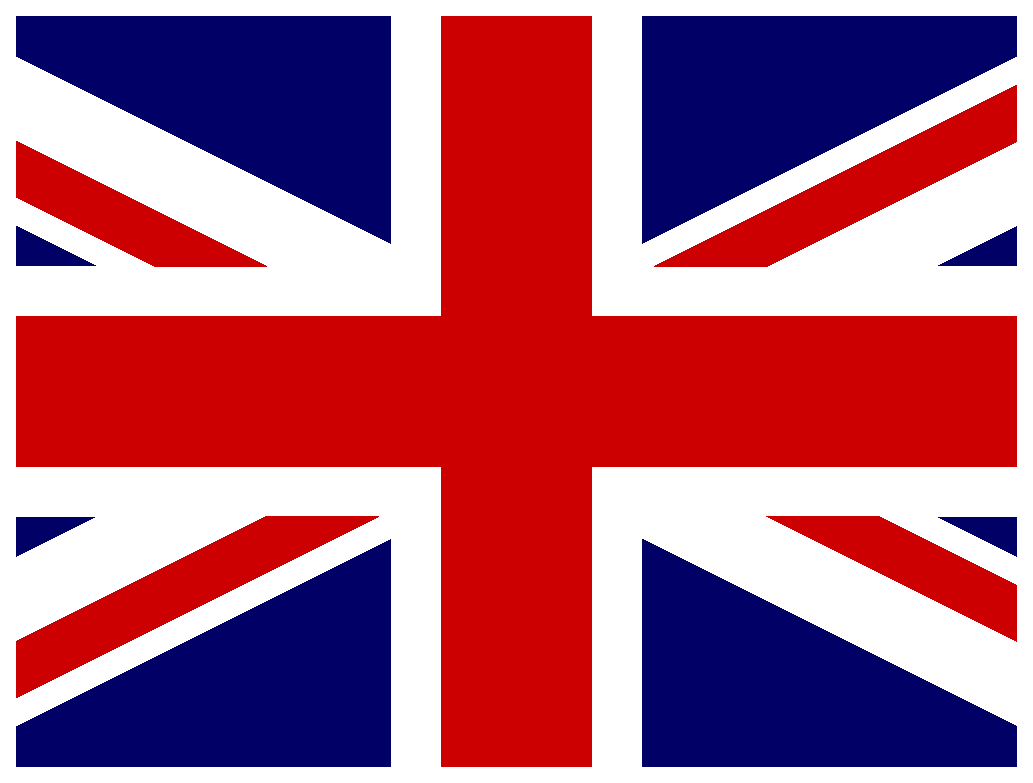
\includegraphics[width=0.15in]{tex/gb.eps}}, BNA  \fbox{
\includegraphics[width=0.15in]{tex/de.eps}}, CII  \fbox{
\includegraphics[width=0.15in]{tex/cn.eps}}...
}%
\item Communication by EMR is done by modulating the carrier waveform:

\begin{tabular}{ccc}%
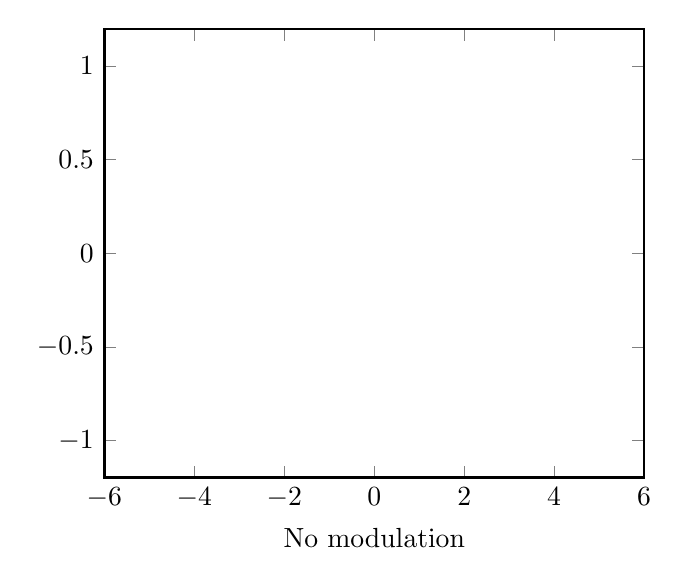
\begin{tikzpicture} % No modulation
	\begin{axis}[smooth,grid=none,scale=1,xlabel={No modulation},line width=1pt,]
		\addplot[white, smooth,xlabel={No modulation},line join=round, line cap=round] {sin(x*20*180/pi)};
	\end{axis}
\end{tikzpicture}&
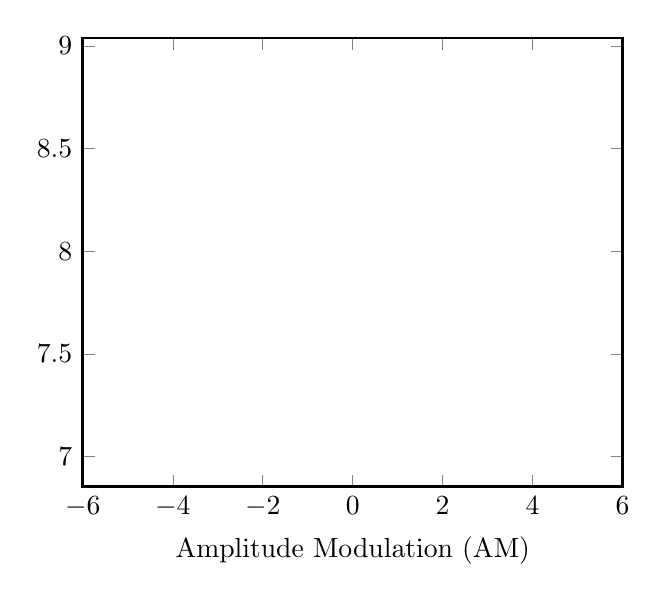
\begin{tikzpicture} %AM
	\begin{axis}[smooth,grid=none,scale=1,xlabel={Amplitude Modulation (AM)},line width=1pt,]
		%\addplot[white, smooth,line join=round, line cap=round] {sin(x*20*180/pi)*sin(x*1*180/pi)};
		\addplot[white, smooth,line join=round, line cap=round] {0.5*sin(x*20*180/pi)*(1+sin(x*1.7*180/pi))+8};

	\end{axis}
\end{tikzpicture}&
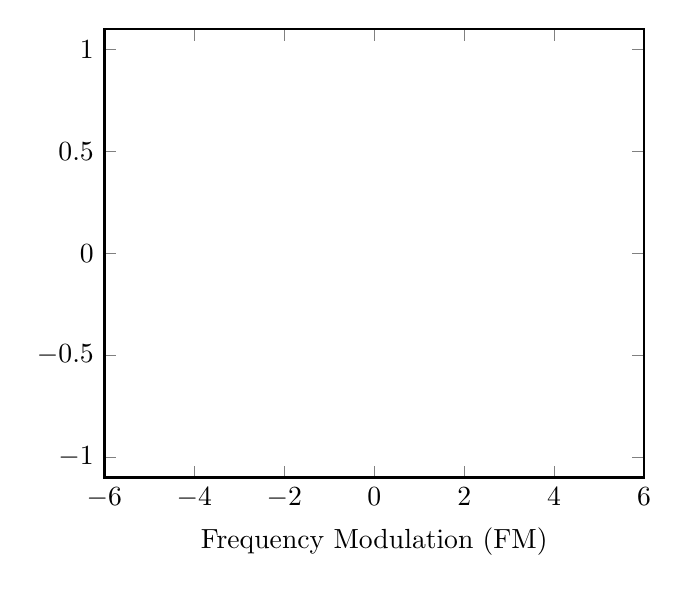
\begin{tikzpicture} % FM
	\begin{axis}[smooth,grid=none,scale=1,xlabel={Frequency Modulation (FM)},line width=1pt,]
		\addplot[white, smooth,line join=round, line cap=round] {sin((x*20 + 6*(sin(x*2*180/pi)))*180/pi)};
	\end{axis}
\end{tikzpicture}
\end{tabular}
%
% \item Not all references agree on the ULF band range, the HAARP range is used here.
%
\item {\bfseries RA}dio {\bfseries D}etecting {\bfseries A}nd {\bfseries R}anging (RADAR) uses microwaves to detect the distance and speed of objects.

\item {\bfseries C}itizens {\bfseries B}and Radio (CB) contains 40 stations between 26.965 - 27.405MHz %\hspace{0.02in}
{% CB Radio
  \definecolor{BoxColor}{rgb}{0.6,0.68,0.86}
  \psframebox[linestyle=none,framesep=1pt,fillcolor=BoxColor,linearc=0]{\black CB}
}.
%
 Schumann resonances are produced in the cavity between the Earth and the ionosphere \hspace{0.02in}%
 \psframebox[fillstyle=none,linestyle=none]{\psscalebox{0.7}{\blip{0,-.07}{S}}}%
 \hspace{0.02in}.
%
 Hydrogen gas emits radio band EMR at 21cm  \hspace{0.05in}%
 \psframebox[fillstyle=none,linestyle=none]{\psscalebox{0.7}{\blip{0,-.07}{H}}}%
 \hspace{0.02in}.
%
 Time / frequency standards shown as \psframebox[linestyle=none] {\rput(0.1in,0){\timestandard}} \hspace{0.1in}.
% 
 Other individual frequencies are represented as icons:\vspace{0.1in}\\
\begin{tabular}{cp{1.4in}cp{1in}cp{1.7in}}
% 
\psframebox[linestyle=none]{\submarine{0.02,.0}{xxHz}}\hspace{0.2in}\vspace{0.05in} & Submarine&
\psframebox[linestyle=none]{\rput(0.15,.05)\pager}&Pager&
\psframebox[linestyle=none]{\rput(0.05,.05){\psframebox[fillstyle=solid,fillcolor=Itinerant,linecolor=Itinerant,linearc=0,framesep=1pt]{\textcolor{Black}{GMRS}}}}&General Mobile Radio Service\\%
%
\psframebox[linestyle=none]{\rput(0.14,0.01){\psframebox[fillstyle=solid,fillcolor=green,linecolor=green,linearc=0]{\textcolor{Black}{xxm}}}}\hspace{.1in}\vspace{0.05in} & Ham / international&
\psframebox[linestyle=none]{\rput(0.14,.03){\weatherstation}\hspace{.03in}\vspace{0.08in}} & Weather&
\psframebox[linestyle=none]{\rput(0.15,.04){
	\psframe[linestyle=solid,linecolor=gray,fillstyle=solid,fillcolor=gray,linearc=0](-.2,-.08)(.2,.08)
	\psframe[hatchwidth=2pt, hatchsep=1.5pt,linestyle=solid,linecolor=yellow,fillstyle=hlines,hatchangle=45,hatchcolor=yellow,fillcolor=gray,linearc=0](-.2,-.08)(.2,.08)
	}
	\hspace{.2in}}\vspace{0.05in}
	& Short wave\\
%
%
\psframebox[linestyle=none]{\rput(0.11,.05){\psframebox[fillstyle=solid,fillcolor=Itinerant,linecolor=Itinerant,linearc=0,framesep=1pt]{\textcolor{Black}{FRS}}}}&Family Radio Service&
\psframebox[linestyle=none]{\rput(0.15,-0.1){\wirelessmic}}&Wireless Mic.&
\psframebox[linestyle=none]{
% 	\rput(0.15,.05){
% 		\psframebox[fillstyle=solid,linearc=0,linecolor=yellow,framesep=1pt,fillcolor=yellow,linewidth=1pt,linestyle=solid]{\textcolor{Black}{CP}}
% 	}
	\rput(0.08, 0.02){
		\psset{linestyle=solid, linewidth=0.02in}
		\psline[linecolor=5GBandColor  ](-.15,0.04)(0.15,0.04)
		\psline[linecolor=4GBandColor ](-.20,0.02)(0.10,0.02)
		\psline[linecolor=3GBandColor](-.10,0.00)(0.20,0.00)
	} 
	\hspace{.03in}\vspace{0.08in}} & Cellular Phones
	\psframebox[fillstyle=solid,linearc=0,linecolor=3GBandColor,framesep=1pt,fillcolor=3GBandColor,linewidth=1pt,linestyle=solid]{\textcolor{Black}{3G}}
	\psframebox[fillstyle=solid,linearc=0,linecolor=4GBandColor, framesep=1pt,fillcolor=4GBandColor, linewidth=1pt,linestyle=solid]{\textcolor{Black}{4G}}
	\psframebox[fillstyle=solid,linearc=0,linecolor=5GBandColor,  framesep=1pt,fillcolor=5GBandColor,  linewidth=1pt,linestyle=solid]{\textcolor{Black}{5G}}
\\
%
% \psframebox[linestyle=none]{
% 	\rput(0.11,.05){
% 		\psframebox[linestyle=none,framesep=1pt,fillcolor=red,linearc=0]{\white SOS}
% 	}
% }
% &
% 	\psset{dotsize=1pt 1}Distress signal, in Morse code:\vspace{0.18in}
% \rput(-1.4,-0.18){
% 	\rput(0,0.05){
% 		\psdots(0,0)(.1,0)(.2,0)\psline{cc-cc}(0.3,0)(0.42,0)\psline{cc-cc}(0.49,0)(0.61,0)\psline{cc-cc}(0.68,0)(0.8,0)\psdots(.9,0)(1,0)(1.1,0)
% 	}
% }%
\end{tabular}
% Slightly modified from this:
%   https://github.com/sikvall/latex-morse

\newcommand{\Mdotlength}{3pt}
\newcommand{\Mdahlength}{9pt}
\newcommand{\Mcharseplength}{9pt}
\newcommand{\Mwordseplength}{21pt}
\newcommand{\Mdiditlength}{6pt}
\newcommand{\Mfetvadd}{1.5pt}
\newcommand{\Mcharsep}{\hspace{9pt}}
\newcommand{\Mwordsep}{\hspace{21pt}}

\newcommand{\dit}{\raisebox{0.5ex}{$\rule{\Mdotlength}{\Mfetvadd}\hspace{\Mdotlength}$}}
\newcommand{\dah}{\raisebox{0.5ex}{$\rule{\Mdahlength}{\Mfetvadd}\hspace{\Mdotlength}$}}

\newcommand{\MCa}{\dit\dah            \Mcharsep}
\newcommand{\MCb}{\dah\dit\dit\dit  \Mcharsep}
\newcommand{\MCc}{\dah\dit\dah\dit   \Mcharsep}
\newcommand{\MCd}{\dah\dit\dit       \Mcharsep}
\newcommand{\MCe}{\dit                \Mcharsep} 
\newcommand{\MCf}{\dit\dit\dah\dit   \Mcharsep}
\newcommand{\MCg}{\dah\dah\dit      \Mcharsep}
\newcommand{\MCh}{\dit\dit\dit\dit   \Mcharsep}
\newcommand{\MCi}{\dit\dit            \Mcharsep}
\newcommand{\MCj}{\dit\dah\dah\dah   \Mcharsep}
\newcommand{\MCk}{\dah\dit\dah       \Mcharsep}
\newcommand{\MCl}{\dit\dah\dit\dit  \Mcharsep}
\newcommand{\MCm}{\dah\dah          \Mcharsep}
\newcommand{\MCn}{\dah\dit          \Mcharsep}
\newcommand{\MCo}{\dah\dah\dah        \Mcharsep}
\newcommand{\MCp}{\dit\dah\dah\dit  \Mcharsep}
\newcommand{\MCq}{\dah\dah\dit\dah \Mcharsep}
\newcommand{\MCr}{\dit\dah\dit      \Mcharsep}
\newcommand{\MCs}{\dit\dit\dit      \Mcharsep}
\newcommand{\MCt}{\dah                \Mcharsep}
\newcommand{\MCu}{\dit\dit\dah       \Mcharsep}
\newcommand{\MCv}{\dit\dit\dit\dah  \Mcharsep}
\newcommand{\MCw}{\dit\dah\dah     \Mcharsep}
\newcommand{\MCx}{\dah\dit\dit\dah  \Mcharsep}
\newcommand{\MCy}{\dah\dit\dah\dah   \Mcharsep}
\newcommand{\MCz}{\dah\dah\dit\dit    \Mcharsep}
\newcommand{\MCAke}{\dit\dah\dah\dit\dah \Mcharsep}
\newcommand{\MCArlig}{\dit\dah\dit\dah   \Mcharsep}
\newcommand{\MCOsten}{\dah\dah\dah\dit   \Mcharsep}
\newcommand{\MCUbel}{\dit\dit\dah\dah    \Mcharsep} % Tyskt Ü
\newcommand{\MCch}{\dah\dah\dah\dah      \Mcharsep} % Tyskt CH

\newcommand{\MPunkt}{\dit\dah\dit\dah\dit\dah           \Mcharsep}
\newcommand{\MSTOP}{\MPunkt}
\newcommand{\MComma}{\dah\dah\dit\dit\dah\dah           \Mcharsep}
\newcommand{\MQuestion}{\dit\dit\dah\dah\dit\dit     \Mcharsep}
\newcommand{\MSlash}{\dah\dit\dit\dah\dit          \Mcharsep}
\newcommand{\MHyphen}{\dah\dit\dit\dit\dit\dah     \Mcharsep}
\newcommand{\MPlus}{\dit\dah\dit\dah\dit          \Mcharsep}
\newcommand{\MColon}{\dah\dah\dah\dit\dit\dit \Mcharsep}
\newcommand{\MApostrophe}{\dit\dah\dah\dah\dah\dit \Mcharsep}
\newcommand{\MQuoteMarks}{\dit\dah\dit\dit\dah\dit \Mcharsep}
\newcommand{\MSOS}{\dit\dit\dit\dah\dah\dah\dit\dit\dit \Mcharsep}

\newcommand{\MRepetera}{\dit\dit\hspace{\Mdiditlength}\dit\dit \Mcharsep}
\newcommand{\MAmpersand}{\dit\dah\dit\dit\dit                     \Mcharsep}
\newcommand{\MAtSign}{\dit\dah\dah\dit\dah\dit            \Mcharsep}
\newcommand{\MEquals}{\dah\dit\dit\dit\dah                \Mcharsep}
\newcommand{\MFelskrivning}{\dit\dit\dit\dit\dit\dit\dit\dit  \Mcharsep}

\newcommand{\MCone}{\dit\dah\dah\dah\dah   \Mcharsep}
\newcommand{\MCtwo}{\dit\dit\dah\dah\dah	  \Mcharsep}
\newcommand{\MCthree}{\dit\dit\dit\dah\dah   \Mcharsep}
\newcommand{\MCfour}{\dit\dit\dit\dit\dah  \Mcharsep}
\newcommand{\MCfive}{\dit\dit\dit\dit\dit   \Mcharsep}
\newcommand{\MCsix}{\dah\dit\dit\dit\dit   \Mcharsep}
\newcommand{\MCseven}{\dah\dah\dit\dit\dit   \Mcharsep}
\newcommand{\MCeight}{\dah\dah\dah\dit\dit  \Mcharsep}
\newcommand{\MCnine}{\dah\dah\dah\dah\dit   \Mcharsep}
\newcommand{\MCzero}{\dah\dah\dah\dah\dah  \Mcharsep}

\newcommand{\MWord}{\MWS}

\lstset{%
literate={A}{\MCa}1
%          {b}{\MBertil}1
%          {c}{\MCesar}1
%          {d}{\MDavid}1
%          {e}{\MErik}1
%          {f}{\MFilip}1
%          {g}{\MGustav}1
%          {h}{\MHelge}1
%          {i}{\MIvar}1
%          {j}{\MJohan}1
%          {k}{\MKalle}1
%          {l}{\MLudvig}1
%          {m}{\MMartin}1
%          {n}{\MNiklas}1
         {O}{\MCo}1
%          {p}{\MPetter}1
%          {q}{\MQvintus}1
%          {r}{\MRudolf}1
         {S}{\MCs}1
%          {t}{\MTore}1
%          {u}{\MUrban}1
%          {v}{\MViktor}1
%          {w}{\MWilhelm}1
%          {x}{\MXerxes}1
%          {y}{\MYngve}1
%          {z}{\MZata}1
         {å}{\MAke}1
         {ä}{\MArlig}1
         {ö}{\MOsten}1
         {.}{\MPunkt}1
         {\ }{\Mwordsep}1
         {,}{\MComma}1
%          {0}{\MNoll}1
}
\newcommand{\morse}[1]{\lstinline{#1}}

International Telecommunication Union (ITU) standard morse code.

% More codes here: https://morsecode.scphillips.com/morse.html
\begin{tabular}{r@{\hspace{.5em}}lr@{\hspace{.5em}}lr@{\hspace{.5em}}lr@{\hspace{.5em}}lr@{\hspace{.5em}}l}
	A & \MCa  & K & \MCk  &U & \MCu   & 0 & \MCzero	& \& &\MAmpersand\\
	B & \MCb  & L & \MCl  &V & \MCv   & 1 & \MCone	&-&\MHyphen\\
	C & \MCc  & M & \MCm  &W & \MCw   & 2 & \MCtwo	& =  &\MEquals \\
	D & \MCd  & N & \MCn  &X & \MCx   & 3 & \MCthree& ,  &\MComma\\
	E & \MCe  & O & \MCo  &Y & \MCy   & 4 & \MCfour	& '  & \MApostrophe\\
	F & \MCf  & P & \MCp  &Z & \MCz   & 5 & \MCfive	& +  & \MPlus\\
	G & \MCg  & Q & \MCq  &  &        & 6 & \MCsix	& ?  &\MQuestion\\
	H & \MCh  & R & \MCr  &. &\MSTOP  & 7 & \MCseven& "  &\MQuoteMarks\\
	I & \MCi  & S & \MCs  &@ &\MAtSign& 8 & \MCeight& /  &\MSlash\\
	J & \MCj  & T & \MCt  &: &\MColon & 9 & \MCnine	& \psframebox[linestyle=none,framesep=1pt,fillcolor=red,linearc=0]{\white SOS} & \MSOS\\
\end{tabular}

%  Kommatecken           & \MKomma        \\
%  Frågetecken (?)       & \MFragetecken  \\
%  Bråktecken (/)        & \MBraktecken   \\
%  Bindestreck (--)      & \MBindestreck  \\
%  Sluttecken (+)        & \MSluttecken   \\
%                        &  \\
%  Repetera              & \MRepetera     \\
%  Väntatecken           & \MVanta        \\
%  Avslutningstecken (+) & \MAvslutning   \\
%  Åtskillnadstecken (=) & \MAtskillnad   \\
%  Felskrivningstecken   & \MFelskrivning \\
%                        &  \\
%                        &  \\
%                        &  \\
%                        &  \\



% \vspace{\baselineskip}



\end{itemize}
}}

    }
  }

  
}
}
	\rput(12.7,15.35){
{
  %Lower Left side notes
  \psset{cornersize=absolute,linearc=4pt,fillstyle=solid,fillcolor=Black, linecolor=white}
  \white

  %\rput[tl]{0}(15.6,14){\psframebox{\parbox[t]{2.3in}{\input{weatherradio.tex}}}}
  %\rput[tl]{0}(15.4,15.8){\psframebox\parbox[t]{2.1in}{\input{satellite.tex}}}}
  %\rput[tl]{0}(18.1,19.4){\psframebox{\parbox[t]{1.3in}{\input{cbradio.tex}}}}

  \newlength{\nLeftSmallWidth}\setlength{\nLeftSmallWidth}{5.44in}

  %Set to the right to make room for the sound banner
  \rput[tl]{0}(0.8,0){
    \parbox[t]{\nLeftSmallWidth}{

	%Description of Sound
	\psframebox{\parbox[t]{\nLeftSmallWidth}{{\Large Sound}
{
\definecolor{HumanAudioColor}{rgb}{0.2,0.2,0.6}
%
\begin{itemize}

\item Although sound, ocean waves, and heartbeats are not electromagnetic, they are included on this chart as a frequency reference. Other properties of electromagnetic waves are different from sound waves.

\item Sound waves are caused by an oscillating compression of molecules. Sound cannot travel in a vacuum such as outer space.

\item The speed of sound in air at sea level is 1240kph (770mph), and much faster in water at 5328kph (3311mph).

% From https://en.wikipedia.org/wiki/Hearing_range
\item Humans can only hear sound between $\approx$20Hz to $\approx$20kHz. Some bats can hear sound up to 200kHz.

\item Infrasound (below 20Hz) can be sensed by internal organs and touch.
%
%from http://www.worldtravelers.org/motionsickness.htm
Frequencies in the 0.2Hz range are often the cause of motion sickness.


\item The 88 piano keys of the Equal Temperament scale are accurately located on the frequency chart. The musical note A (A4 or A440 at 440Hz) is depicted on the chart as \pscirclebox[fillstyle=solid,fillcolor=HumanAudioColor]{\textcolor{white}{A4}}.

\item Over the ages people have striven to divide the continuous audio frequency spectrum into individual musical notes that have harmonious relationships besides the octave. Microtonal musicians study various scales. One recent count lists 4700 different musical scales.

% \textcolor{gray}{\hrule}
% \vspace{.1in}

%\item This image depicts air being compressed as sound waves in a tube from a speaker and then travelling through the tube towards the ear.\\
%%picture of sound
%\vspace{1.75in}
%\rput[t]{0}(1,-.5){\input{pictures/soundwave.tex}}
\end{itemize}
% 	\vspace{0.1in}
% 	%
% 	\begin{tabular}{rl}
% 	%\begin{minipage}[b]{2.45in}\rput(.65,1){\input{pictures/soundwave.tex}}
% 	\begin{minipage}[b]{2.45in}\rput(1.3,.55){\includegraphics[width=2.2in]{pictures/soundbmp.eps}}
% 	\end{minipage}&
% 	\hspace{0.0in}
% 	\begin{minipage}[b]{1.2in}\textcolor{white}{%
% 	This image depicts air being compressed as sound waves in a tube from a speaker and then travelling through the tube towards the ear.\\	}
% 	\end{minipage}
% 	\end{tabular}
% 	\vspace{.2in}
}
}}

	\vspace{\VerticalSeparation}

	%Description of Gravity and gravity waves
	\psframebox{\parbox[t]{\nLeftSmallWidth}{{\white

{\Large Gravitational Waves}

\begin{itemize}

\item Gravity is the mysterious force which holds large objects together and binds our planets, stars, and galaxies together. No links have been established between gravity and electromagnetic radiation or the other physical forces like; the Weak force, the Electromagnetic force, and the Strong force.

\item Gravity is theorized to warp space and time. In fact, gravity is responsible for bending light as observed by the gravity-lens example of distant stars and galaxies.

\item ``Gravitational waves'' appear as ripples in space-time travelling at the speed of light. Long theorized, a gravitational wave was first detected in 2015, and was caused by the merger of two black holes 1.4 billion light years away.

\end{itemize}
}

}}

	\vspace{\VerticalSeparation}

	%Description of Brain waves
	\psframebox{\parbox[t]{\nLeftSmallWidth}{\input{tex/brain.tex}}}

	\vspace{\VerticalSeparation}

	%SI units and measurements
	% Fonts can be a bit larger (\small) instead of \footnote.
	\psframebox{\small\parbox[t]{\nLeftSmallWidth}{%Notes:

%  Symbols here require \usepackage{SIunits}

{\centering

\begin{tabular}{|c|c|l|c|l|}\hline
\multicolumn{5}{|c|}{\bfseries  Système International d'Unités prefixes (SI unit prefixes)}\\ \hline
Symbol & Prefix & Exp. & Name & Multiplier\\ \hline
\rule[0mm]{0mm}{4mm}%
\si{\yotta} & yotta & \si{10\tothe{24}}  & Septillion    & 1,000,000,000,000,000,000,000,000\\
\si{\zetta} & zetta & \si{10\tothe{21}}  & Sextillion    & 1,000,000,000,000,000,000,000\\
\si{\exa}   & exa   & \si{10\tothe{18}}  & Quintillion   & 1,000,000,000,000,000,000\\
\si{\peta}  & peta  & \si{10\tothe{15}}  & Quadrillion   & 1,000,000,000,000,000\\
\si{\tera}  & tera  & \si{10\tothe{12}}  & Trillion      & 1,000,000,000,000\\
\si{\giga}  & giga  & \si{10\tothe{9}}   & Billion       & 1,000,000,000\\
\si{\mega}  & mega  & \si{10\tothe{6}}   & Million       & 1,000,000\\
\si{\kilo}  & kilo  & \si{10\tothe{3}}   & Thousand      & 1,000\\
            &       & \si{10\tothe{0}}   & & 1\\
\si{\milli} & milli & \si{10\tothe{-3}}  & Thousandth    & 0.001\\
\si{\micro} & micro & \si{10\tothe{-6}}  & Millionth     & 0.000 001\\
\si{\nano}  & nano  & \si{10\tothe{-9}}  & Billionth     & 0.000 000 001\\
\si{\pico}  & pico  & \si{10\tothe{-12}} & Trillionth    & 0.000 000 000 001\\
\si{\femto} & femto & \si{10\tothe{-15}} & Quadrillionth & 0.000 000 000 000 001\\
\si{\atto}  & atto  & \si{10\tothe{-18}} & Quintillionth & 0.000 000 000 000 000 001\\
\si{\zepto} & zepto & \si{10\tothe{-21}} & Sextillionth  & 0.000 000 000 000 000 000 001\\
\si{\yocto} & yocto & \si{10\tothe{-24}} & Septillionth  & 0.000 000 000 000 000 000 000 001\\
\hline
\end{tabular}\\
}
% \vspace{0.1in}
{\centering
	\begin{tabular}{cc}
		\begin{tabular}[t]{|c|c|c|}\hline
		\multicolumn{3}{|c|}{\bfseries Measurements on this chart}\\ \hline
		Symbol & Name & Value\\ \hline
		\rule[0mm]{0mm}{4mm}$c$        & Speed of Light                & 2.997 924 58 $\times 10^{8}$ \si{\metre\per\second}\\
		$h$        & Planck's Constant             & 6.626 1 $\times 10^{-34}$  \si{\joule}$\cdot$\si{\second}\\
		$\hbar$    & Planck's Constant (freq)      & 1.054 592 $\times 10^{-34}$  \si{\joule}$\cdot$\si{\second}\\
		\textcolor{FColor}{$f$}        & Frequency (cycles / second) & Hz\\
		\textcolor{WColor}{$\lambda$}  & Wavelength (meters)           & \si{\metre}\\
		\textcolor{EColor}{$E$}        & Energy (Joules)               & J (6.24 $\times 10^{18}$ \si{\electronvolt})\\
		\hline
		\end{tabular}&
		%
		\setlength{\tabcolsep}{2pt}
		\begin{tabular}[t]{|rcl|}\hline
			\multicolumn{3}{|c|}{\bfseries Formulas}\\ \hline
			\rule[0mm]{0mm}{4mm}{\textcolor{EColor}{$E$}}         &=& $h \cdot \textcolor{FColor}{f}$\rule[0.1in]{0in}{0.01in}\\
			\rule[0mm]{0mm}{4mm}{\textcolor{WColor}{$\lambda$}}   &=& $\frac{\D c}{\D \textcolor{FColor}{f}}$\rule[-0.1in]{0in}{0.15in}\\
			\rule[0mm]{0mm}{4mm}{\textcolor{FColor}{$f$}}         &=& $\frac{\D c}{\D \textcolor{WColor}{\lambda}}$\rule[-0.1in]{0in}{0.15in} \\
			\rule{0in}{0.15in}\si{1\angstrom} &=& 0.1\si{\nano\metre}\\
			\rule[0mm]{0mm}{4mm}1\si{\nano\metre}  &=& \si{10\angstrom}\\ \hline
		\end{tabular}
	\end{tabular}\\
}
% \vspace{0.1in}

%
{


}



}}

    }
  }
  
  
}
}
%
	\rput(0, 4.62){
		\psscalebox{0.96}{
			% Left side: 0.55 for symbol edge, 0.25 for margin.
			% Bottom: 0.1 for symbol edge, 0.25 for margin, 3.0 to reach top of page.
			\rput(0.85, 0){%Sources of EMR
%This is displayed as a column of images and text

%The sun and most stars produce a wide range of frequencies in the spectrum (almost filling this entire chart). Many of the frequencies are filtered by our atmosphere.

% Sources shown as images in a vertical strip
{\white

\psset{%old style (pre 2005-07-28
	fillcolor=black,
	fillstyle=solid,
	cornersize=absolute,
	linearc=4pt,
	linestyle=solid,
	linewidth=2pt,
	linecolor=FColor}

\psset{%new style after 2005-07-28
	cornersize=absolute,
	linearc=4pt,
	linestyle=solid,
	linewidth=1pt,
	linecolor=FColor,
	fillstyle=gradient,
	gradangle=0,
	gradbegin=RGBBlackBegin,
	gradend=RGBBlackEnd,
	gradmidpoint=1.0}


\psline(0,0)(0,35.1)

\rput{0}(0,35.1){\psframebox{\parbox[t]
	{0.5in}{\centering Sources of EMR}}}
\rput{0}(0,0.1){\psframebox{\parbox[t]
	{0.5in}{\centering Sources of EMR}}}

\rput{0}(0,3){\psframebox{\parbox[t]
	{0.5in}{\centering
\includegraphics{sources/brain.eps} Human Brain}}}

\rput{0}(0,5.65){\psframebox{\parbox[t]
	{0.5in}{\centering
\includegraphics{sources/powerline.eps} Power Lines (50,60Hz)}}}

%50Hz - 25KHz
\rput{0}(0,7.9){\psframebox{\parbox[t]
	{0.5in}{\centering\includegraphics{sources/induction.eps} Induction Heating}}}

\rput{0}(0,17.6){\psframebox{\parbox[t]
	{0.5in}{\centering\includegraphics{sources/cellphone.eps} Cell phone}}}

% 2.4GHz
\rput{0}(0,18.595){\psframebox{\parbox[t]
	{0.5in}{\centering\includegraphics{sources/microwave.eps} Microwave oven}}}

\rput{0}(0,20){\psframebox{\parbox[t]
	{0.5in}{\centering\includegraphics{sources/radar.eps} Radar}}}

\rput{0}(0,27.2){\psframebox{\parbox[t]
	{0.5in}{\centering\includegraphics{sources/light1.eps} Light bulb}}}

%unneccessary clutter
%\rput{0}(0,27.8){\psframebox{\parbox[t]
%	{0.5in}{\centering\includegraphics{sources/light2.eps} Flourescent light bulb}}}

\rput{0}(0,25){\psframebox{\parbox[t]
	{0.5in}{\centering\includegraphics{sources/people.eps} People}}}

\rput{0}(0,13){\psframebox{\parbox[t]
	{0.5in}{\centering\includegraphics{sources/radio.eps} Radio tower}}}

\rput{0}(0,32){\psframebox{\parbox[t]
	{0.5in}{\centering\includegraphics{sources/xray.eps} X-Ray machines}}}

\rput{0}(0,34){\psframebox{\parbox[t]
	{0.5in}{\centering\includegraphics{sources/radiation.eps} Radioactive elements}}}


}
}

			% Left side: 1.4 for symbol edge, 0.1 for space.
			% Bottom: 0.1 for symbol edge, 0.25 for margin, 3.0 to reach top of page.
			\rput(1.5, 0){% Sizes shown as images in a vertical strip

% from http://www.cellsalive.com/howbig.htm
% hair = 100um
% dust mite = 200um
% ragweed pollen = 20um
% lymphocite = 17um
% red blood cell = 10um
% bakers yeast = 5um
% E. coli bacteria = 3um
% staphylococcus = 800nm
% ebola virus = 1200nm
% rhinovirus = 30nm

% from http://www.brooklyn.cuny.edu/bc/ahp/CellBio/SaS/SandS.html
% bacteria 1um - 5um

% from http://science.howstuffworks.com/virus-human1.htm
% virus = 17 - 300 nm

\psset{%
	fillcolor=white,
	fillstyle=solid,
	cornersize=absolute,
	linearc=4pt,
	fillstyle=solid,
	fillcolor=white,
	linestyle=solid,
	linewidth=1pt,
	linecolor=WColor
}

\psline(0,0)(0,35.1)

\rput{0}(0,35.1){
	\psframebox{\parbox[t]{0.5in}{
		\centering Sizes of EMR}
	}
}
\rput{0}(0,0.1){
	\psframebox{\parbox[t]{0.5in}{
		\centering Sizes of EMR}
	}
}

% 12,756.32 kilometers
\rput{0}(0,5.277){\psframebox{\parbox[t]
	{0.5in}{\centering\includegraphics{sizes/earth.eps} Earth 12,756 km}}}

% 100m
\rput{0}(0,13.758){
\psframebox{\parbox[t]
	{0.5in}{\centering\includegraphics{sizes/field.eps} Football Field 100m}}}

% Buildings (Radio)

% 30 ft (12m)
\rput{0}(0,15.287){
\psframebox{\parbox[t]
	{0.5in}{\centering\includegraphics{sizes/house.eps} House 12m}}}

% 1ft 308mm
\rput{0}(0,17.929){
\psframebox{\parbox[t]
	{0.5in}{\centering\includegraphics{sizes/football.eps} Football 308mm}}}


%from http://hypertextbook.com/facts/2000/DannyDonohue.shtml  from World Book Encyclopedia. Chicago: World Book
%proton diamater is too small to include on this chart
%0.000000000001 mm
%0.000000001 um
%0.000001 nm
%0.001 pm
%1 fm
%
%
%The electron diameter is 1/1000 times smaller than the proton
% 1 atto meter
%
%Also from Pauling, Linus. College Chemistry. San Francisco: Freeman, 1964: 57, 4-5.
% The radius of the electron has not been determined exactly but it is known to be less than 1 x 10-13 cm


%baseball 76mm

% 6ft 1.8m
\rput{0}(0,16.656){
\psframebox{\parbox[t]
	{0.5in}{\centering\includegraphics{sizes/people.eps} People 1.8m}}}% Humans (Radio)


% 1.2cm
\rput{0}(0,20.270){
\psframebox{\parbox[t]
	{0.5in}{\centering\includegraphics{sizes/bee.eps} Honey Bee 1.2cm}}}% Honey Bee (Microwave)

% Pin Head (Infrared)

% dot on page

% Protozoans (Visible)

% 10um Molecules (Ultraviolet)
\rput{0}(0,25.385){
\psframebox{\parbox[t]
	{0.5in}{\centering\includegraphics{sizes/cell.eps} Single Cell \si{10\micro\meter}}}}

\rput{0}(0,32.897){
\psframebox{\parbox[t]
	{0.5in}{\centering\includegraphics{sizes/H2O.eps} Water Molecule \SI{0.3}{\nano\meter}}}}



%3um - 800nm
\rput{0}(0,26.582){
\psframebox{\parbox[t]
	{0.5in}{\centering\includegraphics{sizes/bacteria.eps} Bacteria \si{3\micro\meter} - \si{800\nano\meter}}}}

%protien

%17-300nm
\rput{0}(0,28.374){
\psframebox{\parbox[t]
	{0.5in}{\centering\includegraphics{sizes/virus.eps} Virus \si{17 -} \si{300\nano\meter}}}}

% Atoms (Xray)

% Atomic Nuclei  (Gamma Ray)
}

			%Main section of poster
			% Bottom 0.3 to match up to bottom of sources and sizes, 3.0 to move to top.
			\rput{0}(3.11, 0){\small  % Bands of radio waves (encompassing many other bands)
  %
  %y position = xpos_xvalue/9.8 * 0.5" + nearest xpos_yvalue
  %Ex. xpos results for  750e12 937e12   =    (3.72,27.55)(6.62,27.75)   (5.17,27.65)
  %    3.72/9.8 * 0.5 + 27.5 = 27.690
  %\psframe[fillstyle=solid, fillcolor=BoxColor, linecolor=BoxColor](-0.1,27.690)(9.9,27.838)


  % \wrapuparrow{color}{Ypos 2 decimal places}
  \newcommand{\wrapuparrow}[2]{\rput(9.8,#2){\pscurve[linecolor=#1,fillstyle=none,linewidth=1pt,linestyle=solid]{->}(0,0)(0.1,0.05)(0.02,0.12)}}
  \newcommand{\wrapdnarrow}[2]{\rput(0,#2){\pscurve[linecolor=#1,fillstyle=none,linewidth=1pt,linestyle=solid]{->}(0,0)(-0.1,-0.05)(-0.02,-0.12)}}
  \newcommand{\wrapbtarrow}[2]{
  	\rput(9.8,#2){\pscurve[linecolor=#1,fillstyle=none,linewidth=1pt,linestyle=solid]{->}(0,0)(0.1,0.05)(0.02,0.12)}
  	\rput(0,#2){\pscurve[linecolor=#1,fillstyle=none,linewidth=1pt,linestyle=solid]{->}(0,0)(-0.1,-0.05)(-0.02,-0.12)}}


  %define colors used in this file
  \definecolor{HumanAudioColor}{rgb}{0.2,0.2,0.6}

  \psset{fillstyle=solid,linestyle=none}

  % Bottom end of spectrum fade to black
  \psframe[fillstyle=solid, fillcolor=Black, linecolor=Black](\EMRPositionC,-0.1)(2.9,0.4)
  \psframe[fillstyle=gradient,gradangle=90,gradbegin=Black,gradend=Black,gradmidpoint=1.0,linewidth=0pt,linestyle=none](1.9,-0.1)(2.9,0.4)

  % ULF	Ultra Low Frequency  3 - 30Hz  source  http://www.haarp.alaska.edu/haarp/elf.html
  \psframe[fillcolor=LightRange](\EMRPositionC,3.792)(\EMRPositionE,5.453)

  % ELF	Extremely Low Frequency  30 - 3kHz
  \psframe[fillcolor=DarkRange](\EMRPositionC,5.453)(\EMRPositionE,8.776)

  % VLF	Very Low Frequency	100km - 10km	3kHz - 30kHz
  \psframe[fillcolor=LightRange](\EMRPositionC,8.776)(\EMRPositionE,10.436)

  % LF 	Low Frequency		10km - 1km	30kHz - 300kHz
  \psframe[fillcolor=DarkRange](\EMRPositionC,10.436)(\EMRPositionE,12.097)

  % MF 	Medium frequency 	1km - 100m	300-3000 kHz
  \psframe[fillcolor=LightRange](\EMRPositionC,12.097)(\EMRPositionE,13.758)

  % HF 	High frequency 		100m - 10m	3-30 MHz
  \psframe[fillcolor=DarkRange](\EMRPositionC,13.758)(\EMRPositionE,15.419)

  % VHF	Very High Frequency	10m - 1m	30 - 300 MHz
  \psframe[fillcolor=LightRange](\EMRPositionC,15.419)(\EMRPositionE,17.080)

  % UHF	Ultra High Frequency	1m - 10cm	300MHz - 3GHz
  \psframe[fillcolor=DarkRange](\EMRPositionC,17.080)(\EMRPositionE,18.741)

  % SHF Super High Frequency	10cm - 1cm	3GHz - 30GHz
  \psframe[fillcolor=LightRange](\EMRPositionC,18.741)(\EMRPositionE,20.402)

  % EHF Extremely High Frequency 1cm - 1mm	30GHz - 300GHz
  \psframe[fillcolor=DarkRange](\EMRPositionC,20.402)(\EMRPositionE,22.063)

  % Near Ultraviolet (NUV)		400-300nm  750-1000THz
  \psframe[fillcolor=DarkRange](\EMRPositionC,27.707)(\EMRPositionE,27.916)

  % Medium Ultraviolet (MUV)		300-200nm 1000-1500THz
  \psframe[fillcolor=LightRange](\EMRPositionC,27.916)(\EMRPositionE,28.207)

  % Far Ultraviolet (FUV)		200-100nm 1500-3000THz
  \psframe[fillcolor=DarkRange](\EMRPositionC,28.207)(\EMRPositionE,28.705)

  % Extreme Ultraviolet (EUV)	200-10nm  1500THz - 30PHz
  \psframe[fillcolor=LightRange](\EMRPositionC,28.705)(\EMRPositionE,30.368)


%Large Labels defining the major ranges of EMR
{\large\yellow
\psset{linecolor=yellow,linestyle=solid}
\newlength{\LargeLabelPosition}  \setlength{\LargeLabelPosition}{\EMRPosition+0.55in}
\newlength{\LargeLabelRightPosition}  \setlength{\LargeLabelRightPosition}{\EMRPosition+1.2in}

\newlength{\LargeLabelPositionLeft}  \setlength{\LargeLabelPositionLeft}{\LargeLabelPosition-0.2in}
\newlength{\LargeLabelPositionRight}  \setlength{\LargeLabelPositionRight}{\LargeLabelPosition+0.2in}

\uput[180]{90}(\LargeLabelPosition,34.3){GAMMA RAYS}
\psline[linecolor=LightRange](\EMRPositionC,33.690)(\LargeLabelRightPosition,33.690)
\psline{<->}(\LargeLabelPosition,33.690)(\LargeLabelPosition,35.3)

\psline{<->}(\LargeLabelPosition,33.690)(\LargeLabelPosition,30.368)
\uput[180]{90}(\LargeLabelPosition,32.03){X-RAYS}

\psline{<->}(\LargeLabelPosition,30.368)(\LargeLabelPosition,27.707)
\uput[180]{90}(\LargeLabelPosition,28.65){ULTRAVIOLET}

%760-400nm (394-749 THz)
\psline[linecolor=LightRange](\EMRPositionC,27.243)(\LargeLabelRightPosition,27.243)
\psline{<->}(\LargeLabelPosition,27.707)(\LargeLabelPosition,27.243)
\uput[180]{0}(\LargeLabelPosition,27.48){VISIBLE}

\psline[linecolor=LightRange](\EMRPositionC,23.724)(\LargeLabelRightPosition,23.724)
\psline{<->}(\LargeLabelPosition,27.243)(\LargeLabelPosition,23.724)
\uput[180]{90}(\LargeLabelPosition,25.48){INFRARED}

%0.3GHz bottom
\psline{<->}(\LargeLabelPosition,23.724)(\LargeLabelPosition,17.080)
\uput[180]{90}(\LargeLabelPosition,19.55){MICROWAVE}

\psline{<->}(\LargeLabelPosition,17.080)(\LargeLabelPosition,9.144)
\uput[180]{90}(\LargeLabelPosition,13.11){RADIO WAVES}

}


\psset{linestyle=solid}% put linestyle back to the way it was


%Change below two lines to this for angled lines
\rput{2.92}{%
\pstilt{87.08}{% angle_for_rput = arctan (0.5"/pspicture_width), pstilt_angle = 90-rput_angle

%change above two lines to this for straight lines
%\rput{0}{%
%{

  % Make grid lines
  \multido{\nYPosition=0.0+0.5,\nYEndPosition=0.3+0.5}{69}{%  change the last number here to identify number of rows high
  	  \psline[linecolor=LineGray]{C-C}(0.000,\nYPosition)(0.000,\nYEndPosition)
  	  \psline[linecolor=LineGray]{C-C}(0.817,\nYPosition)(0.817,\nYEndPosition)
  	  \psline[linecolor=LineGray]{C-C}(1.633,\nYPosition)(1.633,\nYEndPosition)
  	  \psline[linecolor=LineGray]{C-C}(2.450,\nYPosition)(2.450,\nYEndPosition)
  	  \psline[linecolor=LineGray]{C-C}(3.267,\nYPosition)(3.267,\nYEndPosition)
  	  \psline[linecolor=LineGray]{C-C}(4.083,\nYPosition)(4.083,\nYEndPosition)
  	  \psline[linecolor=LineGray]{C-C}(4.900,\nYPosition)(4.900,\nYEndPosition)
  	  \psline[linecolor=LineGray]{C-C}(5.717,\nYPosition)(5.717,\nYEndPosition)
  	  \psline[linecolor=LineGray]{C-C}(6.533,\nYPosition)(6.533,\nYEndPosition)
  	  \psline[linecolor=LineGray]{C-C}(7.350,\nYPosition)(7.350,\nYEndPosition)
  	  \psline[linecolor=LineGray]{C-C}(8.167,\nYPosition)(8.167,\nYEndPosition)
  	  \psline[linecolor=LineGray]{C-C}(8.983,\nYPosition)(8.983,\nYEndPosition)
  	  \psline[linecolor=LineGray]{C-C}(9.800,\nYPosition)(9.800,\nYEndPosition)
       \psline[linecolor=white]{C-C}(0,\nYPosition)(9.8,\nYPosition)%
   }
%  \psline[linecolor=LineGray]{C-C}(9.8,-0.5)(9.8,-0.2)% wraparound on first line only


  \uput{2pt}[270]( 4.9,-0.1){\psframebox[fillstyle=solid,fillcolor=FColor,linecolor=FColor]{\textcolor{Black}{Frequency}}}
  \uput{2pt}[270]( 5.7,-0.1){\psframebox[fillstyle=solid,fillcolor=WColor,linecolor=WColor]{\textcolor{Black}{Wavelength}}}
  \uput{2pt}[270]( 6.5,-0.1){\psframebox[fillstyle=solid,fillcolor=EColor,linecolor=EColor]{\textcolor{Black}{Energy}}}


  \newcounter{StartHeight}	\setcounter{StartHeight}{3}
  \newcounter{EndHeight}	\setcounter{EndHeight}{4}

  %From Doug Welch: Crosshatch style for non-visible colors
  \psset{fillstyle=crosshatch,linewidth=0pt,linestyle=none, hatchwidth=2pt, hatchsep=1.5pt}


  % Brain waves
  % Delta waves 0.1 3Hz
  \definecolor{Fill}{rgb}{1,0.9,0.9}\psset{hatchcolor=Fill}
  \psframe(6.55,1.05)(9.80,1.25)\wrapuparrow{Fill}{1.15}
  \psframe(0.00,1.55)(9.80,1.75)\wrapbtarrow{Fill}{1.65}
  \psframe(0.00,2.05)(9.80,2.25)\wrapbtarrow{Fill}{2.15}
  \psframe(0.00,2.55)(9.80,2.75)\wrapbtarrow{Fill}{2.65}
  \psframe(0.00,3.05)(9.80,3.25)\wrapbtarrow{Fill}{3.15}
  \psframe(0.00,3.55)(5.73,3.75)\wrapdnarrow{Fill}{3.65}
  \rput(6.55,1.15){\psframebox[framearc=0.25,fillstyle=solid, fillcolor=Fill,linecolor=Black,framesep=1pt]{0.1Hz}}
  \rput(4.9,2.65){\psframebox[fillstyle=solid,fillcolor=Fill,framesep=1pt]{\boldmath$\delta$ (Delta brain waves)}}
  {\psset{linecolor=yellow,linestyle=solid,linewidth=1pt}
	\psline{<-}(6.55,1.05)(9.80,1.05)
	\psline{-}(0,1.55)(9.80,1.55)
	\psline{-}(0,2.05)(9.80,2.05)
	\psline{-}(0,2.55)(9.80,2.55)
	\psline{-}(0,3.05)(9.80,3.05)
	\psline{->}(0,3.55)(5.73,3.55)
  }

  % Theta 3-8 Hz
  \definecolor{Fill}{rgb}{1,0.8,0.8}\psset{hatchcolor=Fill}
  \psframe(5.73,3.55)(9.8,3.75)\wrapuparrow{Fill}{3.65}
  \psframe(0.00,4.05)(9.8,4.25)\wrapdnarrow{Fill}{4.15}
  \rput(5.73,3.65){\psframebox[framearc=0.25,fillstyle=solid, fillcolor=Fill,linecolor=Black,framesep=1pt]{3Hz}}
  \rput(4.9,4.15){\psframebox[fillstyle=solid,fillcolor=Fill,framesep=1pt]{\boldmath$\theta$ (Theta brain waves)}}
  \rput(9.8,4.15){\psframebox[framearc=0.25,fillstyle=solid, fillcolor=Fill,linecolor=Black]{8Hz}}
  {\psset{linecolor=yellow,linestyle=solid,linewidth=1pt}
	\psline{<-}(5.73,3.55)(9.8,3.55)
	\psline{->}(0.00,4.05)(9.8,4.05)
  }

  % Alpha 8-12Hz
  \definecolor{Fill}{rgb}{1,0.7,0.7}\psset{hatchcolor=Fill}
  \psframe(0.00,4.55)(5.73,4.75)
  \rput(0,4.65){\psframebox[framearc=0.25,fillstyle=solid, fillcolor=Fill,linecolor=Black,framesep=1pt]{8Hz}}
  \rput(2.87,4.65){\psframebox[fillstyle=solid,fillcolor=Fill,framesep=1pt]{\boldmath$\alpha$ (Alpha brain waves)}}
  \psline[linecolor=yellow,linestyle=solid,linewidth=1pt]{<->}(0.00,4.55)(5.73,4.55)

  % Low Beta 12-15
  \definecolor{Fill}{rgb}{1,0.6,0.6}\psset{hatchcolor=Fill}
  \psframe(5.73,4.55)(8.89,4.75)
  \rput(5.73,4.65){\psframebox[framearc=0.25,fillstyle=solid, fillcolor=Fill,linecolor=Black,framesep=1pt]{12Hz}}
  \rput(6.82,4.65){\psframebox[fillstyle=solid,fillcolor=Fill,framesep=1pt]{\boldmath$\beta$ (Low Beta brain waves)}}
  \psline[linecolor=yellow,linestyle=solid,linewidth=1pt]{<->}(5.73,4.55)(8.89,4.55)

  % Mid Beta 15-18
  \definecolor{Fill}{rgb}{1,0.5,0.5}\psset{hatchcolor=Fill}
  \psframe(8.89,4.55)(9.8,4.75)\wrapuparrow{Fill}{4.65}
  \psframe(0.00,5.05)(1.67,5.25)\wrapdnarrow{Fill}{5.15}
  \rput(8.89,4.65){\psframebox[framearc=0.25,fillstyle=solid, fillcolor=Fill,linecolor=Black,framesep=1pt]{15Hz}}
  \rput(0.7,5.15){\psframebox[fillstyle=solid,fillcolor=Fill,framesep=1pt]{\boldmath$\beta$ (Mid Beta brain waves)}}
  {\psset{linecolor=yellow,linestyle=solid,linewidth=1pt}
	\psline{<-}(8.89,4.55)(9.8,4.55)
	\psline{->}(0.00,5.05)(1.67,5.05)
  }

  % High Beta 18-30Hz
  \definecolor{Fill}{rgb}{1,0.4,0.4}\psset{hatchcolor=Fill}
  \psframe(1.67,5.05)(8.89,5.25)
  \rput(1.67,5.15){\psframebox[framearc=0.25,fillstyle=solid, fillcolor=Fill,linecolor=Black,framesep=1pt]{\textcolor{white}{18Hz}}}
  \rput(5.28,5.15){\psframebox[fillstyle=solid,fillcolor=Fill,framesep=1pt]{\boldmath$\beta$ (High Beta brain waves)}}
  \psline[linecolor=yellow,linestyle=solid,linewidth=1pt]{<->}(1.67,5.05)(8.89,5.05)

  % Gamma 30Hz
  \definecolor{Fill}{rgb}{1,0.3,0.3}\psset{hatchcolor=Fill}
  \psframe(8.89,5.05)(9.8,5.25)\wrapuparrow{Fill}{5.15}
  \psframe(0.00,5.55)(3.0,5.75)\wrapdnarrow{Fill}{5.65}
  \psframe[fillstyle=gradient,gradangle=90,gradbegin=Fill,gradend=DarkRange,gradmidpoint=1.0,linewidth=0pt,linestyle=none](3.0,5.55)(4.0,5.75)
  \rput(8.89,5.15){\psframebox[framearc=0.25,fillstyle=solid, fillcolor=Fill,linecolor=Black,framesep=1pt]{\textcolor{white}{30Hz}}}
  \rput(1.5,5.65){\psframebox[fillstyle=solid,fillcolor=Fill,framesep=1pt]{\boldmath$\gamma$ (Gamma brain waves)}}
  {\psset{linecolor=yellow,linestyle=solid,linewidth=1pt}
	\psline{<-}(8.89,5.05)(9.8,5.05)
	\psline{->}(0.00,5.55)(4.0,5.55)
  }

  %The Schumann resonances
  \input{tex/schumann.tex}

  %Power supply transmission frequencies
  \input{tex/power.tex}

  \input{tex/amradio.tex}

  %Middle A musical note 440 Hz
  \rput(7.66,7.16){\pscirclebox[linestyle=solid, linecolor=white, linewidth=1pt, fillstyle=solid,fillcolor=HumanAudioColor]{\textcolor{white}{A4}}}
  %Middle C was 261.63Hz located at \rput(0.31,7.66)

  % Marine Radio 235-325kHz
  %\definecolor{Fill}{rgb}{0.37,0.86,0.86}
  %\psframe[fillstyle=solid, fillcolor=Fill,linewidth=0pt,linestyle=none](8.25,11.60)(9.80,11.75)\wrapuparrow{Fill}{11.65}
  %\psframe[fillstyle=solid, fillcolor=Fill,linewidth=0pt,linestyle=none](0.00,12.10)(3.04,12.25)\wrapdnarrow{Fill}{12.15}
  %\psline{|<*-}(8.25,11.60)(9.8,11.60)
  %\psline{->|*}(0.00,12.10)(3.04,12.10)
  %\uput{1pt}[10](8.25,11.65){235kHz}
  %\rput(1,12.15){Marine Radio}
  %\uput{1pt}[170](3.04,12.15){325kHz}


%For some reason this line cannot be preceded by an \input{} statement
{\yellow

  % GWEN 150 to 175 kHz from http://www.dxing.com/lw.htm
  \psset{fillstyle=solid,linecolor=yellow,linewidth=1pt,linestyle=solid,framesep=0pt,fillcolor=yellow}
  \psline{|<*->|}(1.91,11.55)(4.09,11.55)\rput(3.00,11.55){\psframebox{\textcolor{Black}{Ground Wave Emergency Network}}}

  %155-281kHz from http://www.dxing.com/lw.htm
  \psline{|<*-}(2.37,11.75)(9.8,11.75)\wrapuparrow{yellow}{11.75}\rput(6.09,11.75){\psframebox{\textcolor{Black}{Europe and Asia AM}}}
  \psline{->|}(0.00,12.25)(0.98,12.25)\wrapdnarrow{yellow}{12.25}\rput(.5,12.25){\psframebox{\textcolor{Black}{EU\&Asia AM}}}

  %Radiolocation from OMEGA poster 110-130kHz
  \psline{|<*->|}(7.32,11.05)(9.68,11.05) \rput(8.50,11.05){\psframebox{\textcolor{Black}{Radiolocation}}}
  
  %Maritime Mobile from OMEGA poster 110-190kHz
  \psline{|<*-}(7.32,11.18)(9.8,11.18) \wrapuparrow{yellow}{11.18}\rput(8.50,11.18){\psframebox{\textcolor{Black}{Maritime Mobile}}}
  \psline{->|}(0.00,11.66)(5.25,11.66)\wrapdnarrow{yellow}{11.66}\rput[l](0,11.66){\psframebox{\textcolor{Black}{Maritime Mobile}}}
   
  %160-190kHz from http://www.dxing.com/lw.htm
  %replaced by maritime mobile
  %\psline{|<*->|}(2.82,11.65)(5.25,11.65)  \rput(4.53,11.65){\psframebox{\textcolor{Black}{Open US}}}

  %200-430kHz from http://www.dxing.com/lw.htm
  \psline{|<*-}(5.97,11.55)(9.80,11.55)\wrapuparrow{yellow}{11.55} \rput(7.38,11.55){\psframebox{\textcolor{Black}{Navigational Beacons}}}
  \psline{->|}(0.00,12.05)(7.00,12.05)\wrapdnarrow{yellow}{12.05} \rput(4,12.05){\psframebox{\textcolor{Black}{Navigational Beacons}}}

  %235-325kHz
  \psline{|<*-}(8.25,11.65)(9.80,11.65)\wrapuparrow{yellow}{11.65} \rput(9,11.65){\psframebox{\textcolor{Black}{Marine Radio}}}
  \psline{->|}(0.00,12.15)(3.04,12.15)\wrapdnarrow{yellow}{12.15} \rput(1.5,12.15){\psframebox{\textcolor{Black}{Marine Radio}}}

  %430-500kHz from http://www.dxing.com/lw.htm
  \psline{|<*->|}(7.00,12.05)(9.13,12.05) \rput(8.06,12.05){\psframebox{\textcolor{Black}{Morse code}}}

  %500kHz from http://www.dxing.com/lw.htm
  \rput(9.13,12.2){\psframebox[linestyle=none,framesep=1pt,fillcolor=red]{\white SOS}}

  %500-540kHz from http://www.dxing.com/lw.htm
  \psline{|<*-}(9.13,12.05)(9.8,12.05)\wrapuparrow{yellow}{12.05}
  \psline{->|}(0.00,12.55)(0.42,12.55)\wrapdnarrow{yellow}{12.55} \rput(9.56,12.05){\psframebox{\textcolor{Black}{Beacons}}}

  %from http://www.dxing.com/tuning.htm  1610 to 1700 kHz being the new "X" or "extended" AM band
  \psline{|<*->|}(6.06,13.05)(6.83,13.05) \rput(6.45,13.05){\psframebox{\textcolor{Black}{X-Band}}}

  %from http://www.dxing.com/tuning.htm  1700 to 1800 kHz misc beacons
  \psline{|<*->|}(6.83,13.05)(7.64,13.05) \rput(7.24,13.05){\psframebox{\textcolor{Black}{Beacons}}}

  %1800-2000kHz 160m ham band
  %\psline{<->}(7.64,13.05)(9.13,13.05) \rput(8.38,13.05){\psframebox{\textcolor{Black}{160m}}}

  %from http://www.dxing.com/tuning.htm  2000-2300kHz Marine
  \psline{|<*-}(9.13,13.05)(9.80,13.05)\wrapuparrow{yellow}{13.05}\rput(9.49,13.05){\psframebox{\textcolor{Black}{Marine}}}
  \psline{->|}(0.00,13.57)(1.31,13.57)\wrapdnarrow{yellow}{13.57} \rput(0.94,13.57){\psframebox{\textcolor{Black}{Marine}}}

  %from http://www.dxing.com/tuning.htm  2182kHz distress signal
  \rput(0.56,13.65){\psframebox[linestyle=none,framesep=1pt,fillcolor=red]{\white SOS}}

  %from http://www.dxing.com/tuning.htm  2498-2850 kHz More maritime stations
  \psline{|<*->|}(2.47,13.57)(4.34,13.57) \rput(3.40,13.57){\psframebox{\textcolor{Black}{Marine}}}

  %from http://www.dxing.com/tuning.htm  2850-3150 kHz airplane info
  \psline{|<*->|}(4.34,13.57)(5.75,13.57) \rput(5.04,13.57){\psframebox{\textcolor{Black}{Aeronautical}}}

  %from http://www.dxing.com/tuning.htm  3150 to 3200 kHz: This range is allocated to fixed stations, with most communications in RTTY.
  %\psline{|<*->|}(5.75,13.57)(5.97,13.57) \rput(5.83,13.69){\psframebox{\textcolor{Black}{TTY}}}
  \psframe[linestyle=solid,linecolor=yellow,fillstyle=hlines,hatchangle=45,hatchcolor=yellow](5.75,13.52)(5.97,13.62)

  %from http://www.dxing.com/tuning.htm 3400-3500 kHz: This range is used for aeronautical
  \psline{|<*->|}(6.83,13.57)(7.24,13.57) \rput(7.04,13.57){\psframebox{\textcolor{Black}{Aero}}}
  
  %Loran-C submitted by Poul-Henning Kamp
  \psline{|<*->|}(4.48,11.05)(7.32,11.05) \rput(5.90,11.05){\psframebox{\textcolor{Black}{LORAN-C navigation}}}

  %Radionavigation from OMEGA poster 9-14kHz
  \psline{|<*->|}(1.33,9.55)(7.58,9.55) \rput(4.45,9.55){\psframebox{\textcolor{Black}{Radionavigation}}}
 
  %Maritime Mobile from OMEGA poster 14-19.95kHz
  \psline{|<*-}(7.58,9.55)(9.80,9.55)\wrapuparrow{yellow}{9.55}\rput[l](7.68,9.55){\psframebox{\textcolor{Black}{Maritime Mobile}}}
  \psline{->|}(0.00,10.05)(2.78,10.05)\wrapdnarrow{yellow}{10.05} \rput[l](0,10.05){\psframebox{\textcolor{Black}{Maritime Mobile}}}
 
  %Maritime Mobile from OMEGA poster 20.05-59kHz
  \psline{|<*-}(2.85,10.05)(9.80,10.05)\wrapuparrow{yellow}{10.05}\rput[l](4,10.05){\psframebox{\textcolor{Black}{Maritime Mobile}}}
  \psline{->|}(0.00,10.55)(8.31,10.55)\wrapdnarrow{yellow}{10.55} \rput[l](0.0,10.55){\psframebox{\textcolor{Black}{Maritime Mobile}}}
 
  %Maritime Mobile from OMEGA poster 61-70kHz
  \psline{|<*-}(8.79,10.55)(9.80,10.55)\wrapuparrow{yellow}{10.55}\rput[r](9.8,10.55){\psframebox{\textcolor{Black}{Maritime Mobile}}}
  \psline{->|}(0.00,11.05)(4.48,11.05)\wrapdnarrow{yellow}{11.05} \rput(1,11.05){\psframebox{\textcolor{Black}{Maritime Mobile}}}
 
 
 
 %from http://www.dxing.com/tuning.htm 4000 to 4063 kHz:  mainly used by military forces
  %not enough room to show this one
  %\psline{|<*->|}(9.13,13.57)(9.35,13.57) \rput(9.24,13.57){\psframebox{\textcolor{Black}{MIL}}}

  %4.00-4.438MHz from Radioshack PatrolMan SW-60 shortwave radio guide
  \psline{|<*-}(9.13,13.6)(9.80,13.6)\wrapuparrow{yellow}{13.6} \rput(9.46,13.6){\psframebox{\textcolor{Black}{Marine}}}
  \psline{->|}(0.00,14.1)(0.80,14.1)\wrapdnarrow{yellow}{14.1} \rput(.4,14.1){\psframebox{\textcolor{Black}{Marine}}}

  %from http://www.dxing.com/tuning.htm 4438 to 4650 kHz: This range is mainly used for fixed and mobile
  %\psline{|<*->|}(0.80,14.05)(1.46,14.05)\rput(1.13,14.15){\psframebox{\textcolor{Black}{Fixed \&}}}\rput(1.13,14.05){\psframebox{\textcolor{Black}{Mobile}}}

  %from http://www.dxing.com/tuning.htm 5005 to 5450 kHz: Misc.
  %\psline{|<*->|}(2.50,14.05)(3.70,14.05)\rput(3.10,14.05){\psframebox{\textcolor{Black}{Misc.}}}
  \psframe[linestyle=solid,linecolor=yellow,fillstyle=hlines,hatchangle=45,hatchcolor=yellow](0.80,14.05)(3.70,14.15)

  %from http://www.dxing.com/tuning.htm 5450 to 5730 kHz: This is another band for aeronautical
  \psline{|<*->|}(3.70,14.1)(4.41,14.1)\rput(4.06,14.1){\psframebox{\textcolor{Black}{Aero}}}

  %from http://www.dxing.com/tuning.htm 5730 to 5950 kHz: Misc.
  %\psline{|<*->|}(4.41,14.2)(4.94,14.2)\rput(4.68,14.2){\psframebox{\textcolor{Black}{Misc.}}}
  \psframe[linestyle=solid,linecolor=yellow,fillstyle=hlines,hatchangle=45,hatchcolor=yellow](4.41,14.15)(4.94,14.25)

  %from http://www.dxing.com/tuning.htm 6200 to 6525 kHz: maritime
  \psline{|<*->|}(5.53,14.2)(6.25,14.2)\rput(5.89,14.2){\psframebox{\textcolor{Black}{Marine}}}

  %from http://www.dxing.com/tuning.htm 6525 to 6765 kHz: aeronautical
  \psline{|<*->|}(6.25,14.2)(6.76,14.2)\rput(6.50,14.2){\psframebox{\textcolor{Black}{Aero}}}

  %from http://www.dxing.com/tuning.htm 6765 to 7000 kHz: Misc
  %\psline{|<*->|}(6.76,14.2)(7.24,14.2)\rput(7.00,14.2){\psframebox{\textcolor{Black}{Misc.}}}
  %from http://www.dxing.com/tuning.htm 7300 to 8195 kHz: Misc
  %\psline{|<*->|}(7.83,14.2)(9.47,14.2)\rput(8.65,14.2){\psframebox{\textcolor{Black}{Misc.}}}
  \psframe[linestyle=solid,linecolor=yellow,fillstyle=hlines,hatchangle=45,hatchcolor=yellow](6.76,14.15)(9.47,14.25)

  %from http://www.dxing.com/tuning.htm 8195 to 8815 kHz: maritime
  \psline{|<*-}(9.47,14.2)(9.80,14.2)\wrapuparrow{yellow}{14.2}
  \psline{->|}(0.00,14.75)(0.70,14.75)\wrapdnarrow{yellow}{14.75} \rput(.35,14.75){\psframebox{\textcolor{Black}{Marine}}}

  %from http://www.dxing.com/tuning.htm 8815-9040 kHz: This is another aeronautical
  \psline{|<*->|}(0.70,14.75)(1.06,14.75)\rput(0.88,14.75){\psframebox{\textcolor{Black}{Aero}}}

  %from http://www.dxing.com/tuning.htm 9040-9500kHz international broadcasters.
  %from http://www.dxing.com/tuning.htm 9500 to 9900 kHz: This is the 31-meter international broadcasting
  %from http://www.dxing.com/tuning.htm 9900 to 9995 kHz: International broadcasters, FSK modes
  %from http://www.dxing.com/tuning.htm 10005 to 10100 kHz: This range is used for aeronautical
  %too small to fit in
  \psline{|<*->|}(1.06,14.75)(2.62,14.75)\rput(1.77,14.75){\psframebox{\textcolor{Black}{International}}}

  %from http://www.dxing.com/tuning.htm 10150 to 11175 kHz: International and relays
  \psline{|<*->|}(2.69,14.65)(4.05,14.65)\rput(3.37,14.65){\psframebox{\textcolor{Black}{Intnl. and relays}}}

  %from http://www.dxing.com/tuning.htm 11175 to 11400 kHz: This range is used for aeronautical
  \psline{|<*->|}(4.05,14.65)(4.34,14.65)\rput(4.20,14.75){\psframebox{\textcolor{Black}{Aero}}}

  %from http://www.dxing.com/tuning.htm 11400 to 11650 kHz International
  %\psline{|<*->|}(4.34,14.65)(4.64,14.65)\rput(4.49,14.75){\psframebox{\textcolor{Black}{Intnl}}}
  %from http://www.dxing.com/tuning.htm 11975 to 12330 kHz: This band is primarily used by fixed
  %\psline{|<*->|}(5.03,14.7)(5.45,14.7)\rput(5.24,14.7){\psframebox{\textcolor{Black}{Fixed}}}
  \psframe[linestyle=solid,linecolor=yellow,fillstyle=hlines,hatchangle=45,hatchcolor=yellow](4.34,14.65)(5.45,14.75)

  %from http://www.dxing.com/tuning.htm 12330 to 13200 kHz: This is a busy maritime
  \psline{|<*->|}(5.45,14.7)(6.41,14.7)\rput(5.93,14.7){\psframebox{\textcolor{Black}{Marine}}}

  %Too small and crammed to show
  %from http://www.dxing.com/tuning.htm 13200 to 13360 kHz: Aeronautical
  %\psline{|<*->|}(6.41,14.7)(6.58,14.7)\rput(6.49,14.7){\psframebox{\textcolor{Black}{Aero}}}
  %from http://www.dxing.com/tuning.htm 13360 to 13600 kHz: This range is used by fixed stations,
  %\psline{|<*->|}(6.58,14.7)(6.83,14.7)\rput(6.71,14.7){\psframebox{\textcolor{Black}{Fixed}}}
  %from http://www.dxing.com/tuning.htm 13800 to 14000 kHz: This is used by fixed
  %\psline{|<*->|}(7.04,14.7)(7.24,14.7)\rput(7.14,14.7){\psframebox{\textcolor{Black}{Fixed}}}
  %from http://www.dxing.com/tuning.htm 14350 to 14990 kHz: This segment is used by fixed stations,
  %\psline{|<*->|}(7.59,14.7)(8.21,14.7)\rput(7.90,14.7){\psframebox{\textcolor{Black}{Fixed}}}
  %from http://www.dxing.com/tuning.htm 15010 to 15100 kHz: This range is for aeronautical
  %\psline{|<*->|}(8.23,14.7)(8.31,14.7)\rput(8.27,14.7){\psframebox{\textcolor{Black}{Aero}}}
  %from http://www.dxing.com/tuning.htm 15600 to 16460 kHz: This band is used by fixed
  %\psline{|<*->|}(8.77,14.7)(9.53,14.7)\rput(9.15,14.7){\psframebox{\textcolor{Black}{Fixed}}}
  \psframe[linestyle=solid,linecolor=yellow,fillstyle=hlines,hatchangle=45,hatchcolor=yellow](6.41,14.65)(9.53,14.75)

  %from http://www.dxing.com/tuning.htm 16460 to 17360 kHz: This range is shared between maritime and fixed
  \psline{|<*-}(9.53,14.7)(9.80,14.7)\wrapuparrow{yellow}{14.7}
  \psline{->|}(0.00,15.2)(0.48,15.2)\wrapdnarrow{yellow}{15.2}\rput(0.24,15.2){\psframebox{\textcolor{Black}{Marine}}}

  %from http://www.dxing.com/tuning.htm 17360 to 17550 kHz: The range is shared by aeronautical and fixed
  %\psline{|<*->|}(0.48,15.2)(0.64,15.2)\rput(0.56,15.2){\psframebox{\textcolor{Black}{Aero}}}
  %from http://www.dxing.com/tuning.htm 17900 to 18030 kHz: This band is used for aeronautical
  %\psline{|<*->|}(0.92,15.2)(1.02,15.2)\rput(0.97,15.2){\psframebox{\textcolor{Black}{Aero}}}
  %from http://www.dxing.com/tuning.htm 18030 to 18068 kHz: This range is used by fixed stations
  %\psline{|<*->|}(1.02,15.2)(1.05,15.2)\rput(1.03,15.2){\psframebox{\textcolor{Black}{Fixed}}}
  %from http://www.dxing.com/tuning.htm 18168 to 19990 kHz: Misc.
  %\psline{|<*->|}(1.13,15.2)(2.48,15.2)\rput(1.80,15.2){\psframebox{\textcolor{Black}{Misc}}}
  \psframe[linestyle=solid,linecolor=yellow,fillstyle=hlines,hatchangle=45,hatchcolor=yellow](0.48,15.15)(2.48,15.25)

  %from http://www.dxing.com/tuning.htm 20010 to 21000 kHz: This range is mainly used by fixed stations and a few aeronautical stations
  \psline{|<*->|}(2.49,15.2)(3.17,15.2)\rput(2.83,15.2){\psframebox{\textcolor{Black}{Aero}}}

  %from http://www.dxing.com/tuning.htm 21850 to 22000 kHz: This band is shared by fixed and aeronautical stations
  %\psline{|<*->|}(3.74,15.2)(3.83,15.2)\rput(3.78,15.2){\psframebox{\textcolor{Black}{Aero}}}
  \psframe[linestyle=solid,linecolor=yellow,fillstyle=hlines,hatchangle=45,hatchcolor=yellow](3.74,15.15)(3.83,15.25)

  %from http://www.dxing.com/tuning.htm 22000 to 22855 kHz: This range is reserved for maritime
  \psline{|<*->|}(3.83,15.2)(4.37,15.2)\rput(4.10,15.2){\psframebox{\textcolor{Black}{Marine}}}

  %from http://www.dxing.com/tuning.htm 22855 to 23200 kHz: This band is used by fixed
  %\psline{|<*->|}(4.37,15.2)(4.58,15.2)\rput(4.48,15.2){\psframebox{\textcolor{Black}{Fixed}}}
  %from http://www.dxing.com/tuning.htm 23200 to 23350 kHz: Aeronautical
  %\psline{|<*->|}(4.58,15.2)(4.67,15.2)\rput(4.63,15.2){\psframebox{\textcolor{Black}{Aero}}}
  %from http://www.dxing.com/tuning.htm 23350 to 24890 kHz: This segment is used by fixed stations in FSK and digital modes.
  %\psline{|<*->|}(4.67,15.2)(5.58,15.2)\rput(5.13,15.2){\psframebox{\textcolor{Black}{Fixed}}}
  %from http://www.dxing.com/tuning.htm 25010 to 25550 kHz: This band is used by fixed, mobile, and maritime stations
  %\psline{|<*->|}(5.64,15.2)(5.95,15.2)\rput(5.80,15.2){\psframebox{\textcolor{Black}{Mixed}}}
  %from http://www.dxing.com/tuning.htm 25550 to 25670 kHz: This region is reserved for radio astronomy and is usually free of stations.
  %too small, no room
  %\psline{|<*->|}(5.95,15.2)(6.01,15.2)\rput(5.98,15.2){\psframebox{\textcolor{Black}{Astro}}}
  %from http://www.dxing.com/tuning.htm 26100 to 28000 kHz: This band is used by fixed, mobile, and maritime stations
  %\psline{|<*->|}(6.25,15.2)(7.24,15.2)\rput(6.74,15.2){\psframebox{\textcolor{Black}{Mixed}}}
  %from http://www.dxing.com/tuning.htm 29700 to 30000 kHz: This range is used by low powered fixed and mobile stations
  %\psline{|<*->|}(8.07,15.2)(8.22,15.2)\rput(8.15,15.2){\psframebox{\textcolor{Black}{Mixed}}}
  \psframe[linestyle=solid,linecolor=yellow,fillstyle=hlines,hatchangle=45,hatchcolor=yellow](4.37,15.15)(8.22,15.25)

  %from http://www.dxing.com/tuning.htm 72 to 76 MHz: This range is used for remote control signals for model airplanes and garage door openers, wireless microphones (including those used by law enforcement agencies), and two-way communications inside factories, warehouses, and other industrial facilities. Most channels are spaced at 20 kHz intervals.
  \psframe[framearc=0.25](0.99,16.0)(1.76,16.1)\rput(1.38,16.05){\textcolor{Black}{\tiny Remote Ctrl}}

}

  \input{tex/itinerant.tex}%some extra radio frequencies

  % CB Radio 26.960-27.260 MHz
  \definecolor{BoxColor}{rgb}{0.6,0.68,0.86}
  \psframe[fillstyle=solid, fillcolor=BoxColor,linewidth=0pt,linestyle=none](6.71,15.1)(6.86,15.3)
  %\rput(6.78,15.20){26.960-27.260MHz}
  \rput(6.78,15.2){CB}


  % Digital Television (DTV) Television (Analog) VHF & UHF (Audio??) 54-72MHz
%  \definecolor{BoxColor}{rgb}{0.5,0.68,0.86}
%  \psframe[fillstyle=solid, fillcolor=BoxColor,linewidth=0pt,linestyle=none](6.73,15.55)(9.8,15.65)
%  \psframe[fillstyle=solid, fillcolor=BoxColor,linewidth=0pt,linestyle=none](0.0,16.05)(0.99,16.15)
%  \rput(6.73,15.60){54MHz}
%  \rput(8,15.60){DTV}
%  \rput(0.99,16.10){72MHz}


  % Digital Television (DTV) Television (Analog) VHF & UHF (Audio??) 76-85 MHz
%  \definecolor{BoxColor}{rgb}{0.6,0.68,0.86}
%  \psframe[fillstyle=solid, fillcolor=BoxColor,linewidth=0pt,linestyle=none](1.76,16.05)(3.34,16.15)
%  \rput(1.76,16.10){76MHz}
%  \rput(2.34,16.10){DTV}

  \input{tex/tv.tex}

  % Aeronautical Mobile 108-136 MHz
  \definecolor{BoxColor}{rgb}{0.6,0.68,0.86}
  \psframe[fillstyle=solid, fillcolor=BoxColor,linewidth=0pt,linestyle=none](6.73,16.1)(9.80,16.3)\wrapuparrow{BoxColor}{16.2}
  \psframe[fillstyle=solid, fillcolor=BoxColor,linewidth=0pt,linestyle=none](0.00,16.6)(0.19,16.8)\wrapdnarrow{BoxColor}{16.75}
  \rput(9.07,16.2){Aeronautical}

  \rput(8.39,16.2){\psframebox[linestyle=none,framesep=1pt,fillcolor=red,fillstyle=solid]{\white SOS}}


  %FM radio is placed here since some labels overlap previously defined labels
  \input{tex/fmradio.tex}

  % Marine mobile 162-174 MHz
  \definecolor{BoxColor}{rgb}{0.6,0.86,0.86}
  \psframe[fillstyle=solid, fillcolor=BoxColor,linewidth=0pt,linestyle=none](2.66,16.6)(3.67,16.7)
  %\rput(2.66,16.70){162MHz}
  \rput(3.17,16.65){Marine Mobile}

  % Digital Television (DTV) Television (Analog) VHF & UHF  174-216 MHz
  %\definecolor{BoxColor}{rgb}{0.6,0.8,0.8}
  %\psframe[fillstyle=solid, fillcolor=BoxColor,linewidth=0pt,linestyle=none](3.67,16.55)(6.73,16.65)
  %\rput(3.67,16.6){174MHz}
  %\rput(5.20,16.6){Digital Television}


%54-216 MHz  VHF  (***spread this line over many rows!)


  % SuperBand - CATV ch 23-36 (216-300 MHz)
%  \definecolor{BoxColor}{rgb}{0.8,0.68,0.86}
%  \psframe[fillstyle=solid, fillcolor=BoxColor,linewidth=0pt,linestyle=none](6.73,16.55)(9.8,16.65)
%  \psframe[fillstyle=solid, fillcolor=BoxColor,linewidth=0pt,linestyle=none](0.0,17.05)(1.57,17.15)
%  \rput(6.73,16.60){216MHz}
%  \rput(8,16.60){SuperBand - CATV ch 23-36}

  %from http://www.dxing.com/above30.htm 225 to 400 MHz: This very wide band is used for military aviation communications in AM. Most channels are 100 kHz apart.
  \definecolor{BoxColor}{rgb}{0.6,0.68,0.86}
  \psframe[fillstyle=solid, fillcolor=BoxColor,linewidth=0pt,linestyle=none](7.30,16.6)(9.80,16.8)\wrapuparrow{BoxColor}{16.7}
  \psframe[fillstyle=solid, fillcolor=BoxColor,linewidth=0pt,linestyle=none](0.00,17.2)(5.64,17.3)\wrapdnarrow{BoxColor}{17.25}
  \rput(9.07,16.7){Military}
  \rput(8.39,16.7){\psframebox[linestyle=none,framesep=1pt,fillcolor=red,fillstyle=solid]{\white SOS}}
  \rput(2.82,17.25){Military}

%from http://www.dxing.com/above30.htm 400 to 406 MHz: This range is used primarily by government and military stations in FM.
%from http://www.dxing.com/above30.htm 406 to 420 MHz: In the United States, this band is used exclusively by the federal government. All transmissions are in FM, with most channels spaced at 25 kHz intervals.
  \definecolor{BoxColor}{rgb}{0.9,0.68,0.86}
  \psframe[fillstyle=solid, fillcolor=BoxColor,linewidth=0pt,linestyle=none](5.64,17.2)(6.33,17.35) \rput(6.15,17.28){Gov}
  \rput(5.85,17.27){\psframebox[linestyle=none,framesep=1pt,fillcolor=red,fillstyle=solid]{\white SOS}}


  % HyperBand-CATV Ch 37-62 (300-456 MHz)
%  \definecolor{BoxColor}{rgb}{0.9,0.68,0.86}
%  \psframe[fillstyle=solid, fillcolor=BoxColor,linewidth=0pt,linestyle=none](1.57,17.05)(7.49,17.15)
%  %\rput(1.57,17.25){300MHz}
%  \rput(4.16,17.10){HyperBand-CATV Ch 37-62}


  % UHF Band Ch 14-83 (470-890 MHz)
  %\definecolor{BoxColor}{rgb}{0.9,0.68,0.86}
  %\psframe[fillstyle=solid, fillcolor=BoxColor,linewidth=0pt,linestyle=none](7.92,17.05)(9.80,17.15)
  %\psframe[fillstyle=solid, fillcolor=BoxColor,linewidth=0pt,linestyle=none](0.0,17.55)(7.15,17.65)
  %\rput(4.16,17.60){UHF Band Ch 14-83}

  \input{tex/ham.tex}

  % Microwave bands (notice even octave spacing on most bands)
  \psset{fillstyle=crosshatch,linewidth=0pt,linestyle=none}


  % Microwave P-band (0.3-1 GHz)
  \definecolor{Fill}{rgb}{0.1,0.1,0.67}\psset{hatchcolor=Fill}
  \psframe(1.57,17.0)(9.8,17.1)\wrapuparrow{Fill}{17.05}
  \psframe(0.0,17.5)(8.79,17.6)\wrapdnarrow{Fill}{17.55}
%   \rput(1.57,17.05){\textcolor{white}{0.3GHz}}
  \rput(1,17.55){\psframebox[fillstyle=solid,fillcolor=Fill,framesep=1pt]{\textcolor{white}{\tiny Microwave P-band (Previous)}}}

  % Microwave L-band (1-2 GHz)
  \definecolor{Fill}{rgb}{0.2,0.1,0.67}\psset{hatchcolor=Fill}
  \psframe(8.79,17.55)(9.8,17.75)\wrapuparrow{Fill}{17.65}
  \psframe(0.0,18.05)(8.79,18.25)\wrapdnarrow{Fill}{18.15}
  \psdots[linewidth=1.2pt,linecolor=white,linestyle=none, fillcolor=white, dotstyle=triangle*](8.79,17.52)
  \rput(8.79,17.75){\textcolor{white}{1GHz}}
%   \rput(4,18.14){\psframebox[fillstyle=solid,fillcolor=Fill,framesep=2pt]{\textcolor{white}{Microwave L-band (Long)}}}
  \rput(4.715,18.14){\psframebox[fillstyle=solid,fillcolor=Fill,framesep=2pt]{\textcolor{white}{Microwave L-band}}}
  \rput(5.825,18.14){\psframebox[fillstyle=solid,fillcolor=Fill,framesep=2pt]{\textcolor{white}{(Long)}}}

  %Hydrogen line at 21cm (1.42758313333 GHz)
  %Idea from Douglas Scott
  %Info from http://www.drao-ofr.hia-iha.nrc-cnrc.gc.ca/outreach/skygazing/1997/sep1197.html
  \blip{4.03,18}{H}

  \input{tex/catv.tex}
  
  
  % Cell phone 800MHz (Time division multiple access (TDMA)) not actuially 800MHz, and already covered in the 3G list
%   \rput(5.64,17.5){\psframebox[fillstyle=solid,linecolor=yellow,framesep=0pt,fillcolor=yellow,linewidth=1pt,linestyle=solid]{\textcolor{Black}{CP}}}
  %from http://www.dxing.com/tuning.htm 825-894MHz cell phone including 850MHz GSM phones
  %(Frequency division multiple access (FDMA))
%   \psline[linecolor=yellow,linewidth=1pt,linestyle=solid]{|<*->|}(6.07,17.5)(7.21,17.5)
%   \rput(6.64,17.5){\psframebox[fillstyle=solid,linecolor=yellow,framesep=0pt,fillcolor=yellow,linewidth=1pt,linestyle=solid]{\textcolor{Black}{CP}}}

  % Cell phone 1.8GHz (GSM phone)
%   \rput[b](7.30,18.0){\psframebox[fillstyle=solid,linecolor=yellow,framesep=0pt,fillcolor=yellow,linewidth=1pt,linestyle=solid]{\textcolor{Black}{CP}}}

  % Cell phone 1.9GHz
  %\rput[b](8.07,18.0){\psframebox[fillstyle=solid,linecolor=yellow,framesep=0pt,fillcolor=yellow,linewidth=1pt,linestyle=solid]{\textcolor{Black}{CP}}}

  % Code division multiple access (CDMA) 1850-1990MHz (PCS phones)
  % notes from from http://electronics.howstuffworks.com/cell-phone8.htm
%   \psline[linecolor=yellow,linewidth=1pt,linestyle=solid]{|<*->|}(7.69,18.0)(8.72,18.0)
%   \rput[b](8.21,18.0){\psframebox[fillstyle=solid,linecolor=yellow,framesep=0pt,fillcolor=yellow,linewidth=1pt,linestyle=solid]{\textcolor{Black}{CP}}}


  %from:
  % - Radioshack PatrolMan SW-60 shortwave radio guide
  % - http://www.dxing.com/tuning.htm 
  % - Poul-Henning Kamp
  % - OMEGA poster
  \rput(2.81,10.15){\timestandard}% 20.0 kHz  Standard Frequency and Time Signal from OMEGA poster
  \rput(8.55,10.65){\timestandard}% 60.0 kHz  WWVB-USA, MSF-UK  time signal transmissions.
  \rput(1.91,11.15){\timestandard}% 75.0 kHz  Swiss time signal transmission
  \rput(2.37,11.15){\timestandard}% 77.5 kHz  DCF77 - German time signal transmission 
  \rput(2.48,13.70){\timestandard}% 2.5MHz
  \rput(6.54,13.70){\timestandard}% 3.33MHz Canadian
  \rput(2.48,14.15){\timestandard}% 5MHz
  \rput(7.90,14.15){\timestandard}% 7.335MHz Canadian
  \rput(2.48,14.65){\timestandard}% 10MHz
  \rput(7.90,14.65){\timestandard}% 14.670MHz Canadian
  \rput(8.22,14.65){\timestandard}% 15MHz
  \rput(2.48,15.15){\timestandard}% 20MHz Reception here is usually possible only in daytime.
  \rput(5.64,15.15){\timestandard}% 25MHz This range is for standard time and frequency stations, although none are currently operating here.

  %Weather stations
  \rput(9.46,12.2){\weatherstation}%512kHz
  \rput(0.29,16.7){\weatherstation}%137MHz
  \rput(2.70,16.55){\weatherstation}%162.48MHz


  % Microwave S-band (2-4 GHz)
  \definecolor{Fill}{rgb}{0.3,0.1,0.67}\psset{hatchcolor=Fill}
  \psframe(8.79,18.05)(9.8,18.25)\wrapuparrow{Fill}{18.15}
  \psframe(0.0,18.55)(8.79,18.75)\wrapdnarrow{Fill}{18.65}
  \psdots[linewidth=1.2pt,linecolor=white,linestyle=none, fillcolor=white, dotstyle=triangle*](8.79,18.02)
  \rput(8.79,18.14){\textcolor{white}{2GHz}}
  \rput(5.5,18.65){\psframebox[fillstyle=solid,fillcolor=Fill,framesep=2pt]{\textcolor{white}{Microwave S-band (Short)}}}

  %water absorption band at 2.4GHz water (that's why microwave ovens use that band). Thanks to Poul-Henning Kamp 
% Later proven wrong by Anders J. Johansson (20060219)
%   \rput(0.57,18.55){
%   \psclip{\psframe[fillstyle=none,linestyle=none](0,0)(2.4,.3)}
%     \pscurve[fillstyle=crosshatch,hatchcolor=Black,hatchangle=180,hatchwidth=0.5pt,hatchsep=1pt,fillcolor=blue,linecolor=Black,linestyle=solid]
% 	(0,.2)(.5,.15)(1,.02)(1.5,.15)(2,0.2)
%     \rput(.5,.2){\psframebox[framesep=1pt,framearc=0.2,fillstyle=solid, fillcolor=Black,linewidth=0pt,linestyle=none]{\textcolor{white}{Water absorption}}}
% 
%   \endpsclip}

  % Microwave C-band (4-8 GHz)
  \definecolor{Fill}{rgb}{0.4,0.1,0.67}\psset{hatchcolor=Fill}
  \psframe(8.79,18.55)(9.8,18.75)\wrapuparrow{Fill}{18.65}
  \psframe(0.0,19.05)(8.79,19.25)\wrapdnarrow{Fill}{19.15}
  \psdots[linewidth=1.2pt,linecolor=white,linestyle=none, fillcolor=white, dotstyle=triangle*](8.79,18.52)
  \rput(8.79,18.77){\textcolor{white}{4GHz}}
  \rput(5.5,19.15){\psframebox[fillstyle=solid,fillcolor=Fill,framesep=2pt]{\textcolor{white}{Microwave C-band (Compromise)}}}

  %Wireless LAN   Frequency Range; 2.4GHz to 2.5GHz , 5.15GHz to 5.875GHz  (From D-Link Air expert card, good for America and Europe)
  %2.4GHz to 2.5GHz
  \psframe[fillstyle=solid, fillcolor=gray](1.57,18.67)(2.15,18.77)\rput(1.86,18.72){\textcolor{yellow}{W-LAN}}
  %5.15GHz to 5.875GHz
  \psframe[fillstyle=solid, fillcolor=gray](2.57,19.15)(4.43,19.25)\rput(3.50,19.20){\textcolor{yellow}{Wireless LAN}}

 
 %MVDDS/ITFS (Multichannel Multipoint Data Service/ Instructional Television Fixed Service, Thanks to Ranjan Acharya (source IEE spectrum March 2004) 2.5-2.7GHz
{
	\tiny
	\psframe[fillstyle=solid,linestyle=solid,linecolor=Black,linewidth=1pt,framearc=0.25,fillcolor=red](2.15,18.67)(3.24,18.77)
	\rput(2.69,18.72){\textcolor{white}{ITFS}}
}
  
% Satellite Radio (too crowded to show properly)
%Sirius 2320-  2332.5  MHz 
%\psframe[fillstyle=solid, fillcolor=blue,linewidth=0pt,linestyle=none](1.09,18.55)(1.17,18.75)
%XM  Radio 2332.5-  2345  MHz
%\psframe[fillstyle=solid, fillcolor=blue,linewidth=0pt,linestyle=none](1.17,18.55)(1.24,18.75)




{%C-Band satellite channels
\newlength{\nCBANDOddYOffset} \setlength{\nCBANDOddYOffset}{18.60in}
\newlength{\nCBANDEvenYOffset} \setlength{\nCBANDEvenYOffset}{\nCBANDOddYOffset+0.08in}
\tiny
  \psset{framesep=1pt,framearc=.25,fillcolor=green,fillstyle=solid}
  \rput(7.77,\nCBANDOddYOffset){\psframebox{01}}	%3720MHz
  \rput(7.84,\nCBANDEvenYOffset){\psframebox{02}}	%3740
  \rput(7.92,\nCBANDOddYOffset){\psframebox{03}}	%3760
  \rput(7.99,\nCBANDEvenYOffset){\psframebox{04}}	%3780
  \rput(8.07,\nCBANDOddYOffset){\psframebox{05}}	%3800
  \rput(8.14,\nCBANDEvenYOffset){\psframebox{06}}	%3820
  \rput(8.22,\nCBANDOddYOffset){\psframebox{07}}	%3840
  \rput(8.29,\nCBANDEvenYOffset){\psframebox{08}}	%3860
  \rput(8.36,\nCBANDOddYOffset){\psframebox{09}}	%3880
  \rput(8.44,\nCBANDEvenYOffset){\psframebox{10}}	%3900
  \rput(8.51,\nCBANDOddYOffset){\psframebox{11}}	%3920
  \rput(8.58,\nCBANDEvenYOffset){\psframebox{12}}	%3940
  \rput(8.65,\nCBANDOddYOffset){\psframebox{13}}	%3960
  \rput(8.72,\nCBANDEvenYOffset){\psframebox{14}}	%3980
  \rput(8.79,\nCBANDOddYOffset){\psframebox{15}}	%4000
  \rput(8.86,\nCBANDEvenYOffset){\psframebox{16}}	%4020
  \rput(8.93,\nCBANDOddYOffset){\psframebox{17}}	%4040
  \rput(9.00,\nCBANDEvenYOffset){\psframebox{18}}	%4060
  \rput(9.07,\nCBANDOddYOffset){\psframebox{19}}	%4080
  \rput(9.14,\nCBANDEvenYOffset){\psframebox{20}}	%4100
  \rput(9.21,\nCBANDOddYOffset){\psframebox{21}}	%4120
  \rput(9.28,\nCBANDEvenYOffset){\psframebox{22}}	%4140
  \rput(9.35,\nCBANDOddYOffset){\psframebox{23}}	%4160
  \rput(9.42,\nCBANDEvenYOffset){\psframebox{24}}	%4180
}

  % Microwave X-band (8-12.5 GHz)
  \definecolor{Fill}{rgb}{0.5,0.1,0.67}\psset{hatchcolor=Fill}
  \psframe(8.79,19.05)(9.8,19.25)\wrapuparrow{Fill}{19.15}
  \psframe(0.0,19.55)(5.30,19.75)\wrapdnarrow{Fill}{19.65}
  \psdots[linewidth=1.2pt,linecolor=white,linestyle=none, fillcolor=white, dotstyle=triangle*](8.79,19.02)
  \rput(8.79,19.15){\textcolor{white}{8GHz}}
  \rput(3.25,19.65){\psframebox[fillstyle=solid,fillcolor=Fill,framesep=2pt]{\textcolor{white}{Microwave X-band (X marks the spot)}}}

  % Microwave Ku-band (12.5-18 GHz)
  \definecolor{Fill}{rgb}{0.6,0.1,0.67}\psset{hatchcolor=Fill}
  \psframe(5.30,19.55)(9.8,19.75)\wrapuparrow{Fill}{19.65}
  \psframe(0.0,20.05)(0.66,20.25)\wrapdnarrow{Fill}{20.15}
  \psline[linecolor=Black,linewidth=1pt,linestyle=solid](5.30,19.55)(5.30,19.75)
  \psdots[linewidth=1.2pt,linecolor=white,linestyle=none, fillcolor=white, dotstyle=triangle*](5.30,19.52)
  \rput(5.30,19.65){\textcolor{white}{12.5GHz}}
  \rput(8.4,19.65){\psframebox[fillstyle=solid,fillcolor=Fill,framesep=2pt]{\textcolor{white}{Microwave Ku-band (Kurtz Under)}}}

  % Microwave K-band (18-27.25 GHz)
  \definecolor{Fill}{rgb}{0.7,0.1,0.67}\psset{hatchcolor=Fill}
  \psframe(0.66,20.05)(6.52,20.25)
  \psline[linecolor=Black,linewidth=1pt,linestyle=solid](0.66,20.05)(0.66,20.25)
  \psdots[linewidth=1.2pt,linecolor=white,linestyle=none, fillcolor=white, dotstyle=triangle*](0.66,20.02)
  \rput(0.66,20.15){\textcolor{white}{18GHz}}
  \rput(1.85,20.15){\psframebox[fillstyle=solid,fillcolor=Fill,framesep=2pt]{\textcolor{white}{Microwave K-band (Kurtz)}}}



{%K-Band satellite channels ref: "Telesat, Anik F3 Ku-Band Channel Centre Frequencies"
\small
% \newlength{\KBA}  \setlength{\KBA}{19.52in} %vertical position of kBand channels 1-16
% \newlength{\KBB}  \setlength{\KBB}{19.57in} %vertical position of kBand channels 17-32

  \psset{framesep=1pt,fillcolor=BrightGreen,fillstyle=solid,dotstyle=triangle,linecolor=BrightGreen}
% Upload channels 1-16
	\psdots(6.921,19.57)	% 14014750000.00Hz
	\psdots(6.952,19.57)	% 14045250000.00Hz
	\psdots(6.982,19.57)	% 14075750000.00Hz
	\psdots(7.013,19.57)	% 14106250000.00Hz
	\psdots(7.044,19.57)	% 14136750000.00Hz
	\psdots(7.074,19.57)	% 14167250000.00Hz
	\psdots(7.104,19.57)	% 14197750000.00Hz
	\psdots(7.135,19.57)	% 14228250000.00Hz
	\psdots(7.165,19.57)	% 14258750000.00Hz
	\psdots(7.195,19.57)	% 14289250000.00Hz
	\psdots(7.225,19.57)	% 14319750000.00Hz
	\psdots(7.255,19.57)	% 14350250000.00Hz
	\psdots(7.286,19.57)	% 14380750000.00Hz
	\psdots(7.315,19.57)	% 14411250000.00Hz
	\psdots(7.345,19.57)	% 14441750000.00Hz
	\psdots(7.375,19.57)	% 14472250000.00Hz
% Download channels 17-32
	\psdots(6.934,19.52)	% 14027750000.00Hz
	\psdots(6.965,19.52)	% 14058250000.00Hz
	\psdots(6.995,19.52)	% 14088750000.00Hz
	\psdots(7.026,19.52)	% 14119250000.00Hz
	\psdots(7.057,19.52)	% 14149750000.00Hz
	\psdots(7.087,19.52)	% 14180250000.00Hz
	\psdots(7.117,19.52)	% 14210750000.00Hz
	\psdots(7.148,19.52)	% 14241250000.00Hz
	\psdots(7.178,19.52)	% 14271750000.00Hz
	\psdots(7.208,19.52)	% 14302250000.00Hz
	\psdots(7.238,19.52)	% 14332750000.00Hz
	\psdots(7.268,19.52)	% 14363250000.00Hz
	\psdots(7.298,19.52)	% 14393750000.00Hz
	\psdots(7.328,19.52)	% 14424250000.00Hz
	\psdots(7.358,19.52)	% 14454750000.00Hz
	\psdots(7.388,19.52)	% 14485250000.00Hz

%Draw a little Ku satellite
\rput{15}(5.93,19.75){
  \psset{framesep=1pt,framearc=0,fillcolor=BrightGreen,fillstyle=solid,dotstyle=triangle,linewidth=.01in,linestyle=solid,linecolor=BrightGreen}
  \psline(-0.14,0)(0.14,0)
  \pscircle(0,0){0.035}
  \psframe(-.14,.02)(-.06,-.02)
  \psframe(.14,.02)(.06,-.02)
}
  \rput[t](5.93,19.68){\textcolor{BrightGreen}{Ku-band TV}}

%draw arrows showing signal in/out
{\psset{linecolor=BrightGreen,fillstyle=none,linewidth=1pt,linestyle=solid,linearc=.06}
 \psline{->}(7.148,19.60)(7.148,19.75)(6.08,19.75)
 \psline{->}(5.78,19.75)(4.6575,19.75)(4.6575,19.60)
}


% Download channels 1-16
	\psset{dotangle=180}
	\psdots(4.387,19.57)	% 11714750000.00Hz
	\psdots(4.423,19.57)	% 11745250000.00Hz
	\psdots(4.460,19.57)	% 11775750000.00Hz
	\psdots(4.497,19.57)	% 11806250000.00Hz
	\psdots(4.533,19.57)	% 11836750000.00Hz
	\psdots(4.569,19.57)	% 11867250000.00Hz
	\psdots(4.606,19.57)	% 11897750000.00Hz
	\psdots(4.642,19.57)	% 11928250000.00Hz
	\psdots(4.678,19.57)	% 11958750000.00Hz
	\psdots(4.714,19.57)	% 11989250000.00Hz
	\psdots(4.750,19.57)	% 12019750000.00Hz
	\psdots(4.786,19.57)	% 12050250000.00Hz
	\psdots(4.822,19.57)	% 12080750000.00Hz
	\psdots(4.857,19.57)	% 12111250000.00Hz
	\psdots(4.893,19.57)	% 12141750000.00Hz
	\psdots(4.928,19.57)	% 12172250000.00Hz
% Download channels 17-32
	\psdots(4.402,19.52)	% 11727750000.00Hz
	\psdots(4.439,19.52)	% 11758250000.00Hz
	\psdots(4.476,19.52)	% 11788750000.00Hz
	\psdots(4.512,19.52)	% 11819250000.00Hz
	\psdots(4.549,19.52)	% 11849750000.00Hz
	\psdots(4.585,19.52)	% 11880250000.00Hz
	\psdots(4.621,19.52)	% 11910750000.00Hz
	\psdots(4.657,19.52)	% 11941250000.00Hz
	\psdots(4.693,19.52)	% 11971750000.00Hz
	\psdots(4.729,19.52)	% 12002250000.00Hz
	\psdots(4.765,19.52)	% 12032750000.00Hz
	\psdots(4.801,19.52)	% 12063250000.00Hz
	\psdots(4.837,19.52)	% 12093750000.00Hz
	\psdots(4.872,19.52)	% 12124250000.00Hz
	\psdots(4.908,19.52)	% 12154750000.00Hz
	\psdots(4.943,19.52)	% 12185250000.00Hz
}



  %water absorption line at 22GHz
% (3.5,20.05) -1.2x
  \rput(2.3,20.05){
  \psclip{\psframe[fillstyle=none,linestyle=none](0,0)(2.4,.3)}
    \pscurve[fillstyle=crosshatch,hatchcolor=Black,hatchangle=180,hatchwidth=0.5pt,hatchsep=1pt,fillcolor=blue,linecolor=Black,linestyle=solid]
	(0,.2)(.75,.15)(1,.02)(1.25,.15)(2,0.2)
    \rput(1,.2){\psframebox[framesep=1pt,framearc=0.2,fillstyle=solid, fillcolor=Black,linewidth=0pt,linestyle=none]{\textcolor{white}{Water absorption 22GHz}}}
  \endpsclip}

{
	% Cordless phone 2.4GHz
	\psset{fillstyle=none, linecolor=yellow,linestyle=solid, linewidth=1pt, linearc=.05}
	\rput[r](1.47,18.62){\textcolor{yellow}{Cordless phone 2.4GHz}}
	\psline{-*}(1.50,18.62)(1.57,18.62)(1.57,18.5)
	%     
	% Microwave oven 2.45GHz
	\rput[l](1.96,18.62){\textcolor{yellow}{2.45GHz Microwave Oven}}
	\psline{-*}(1.92,18.62)(1.86,18.62)(1.86,18.5)
}

  % Microwave Ka-band (27.25 - 36 GHz)
  \definecolor{Fill}{rgb}{0.8,0.1,0.67}\psset{hatchcolor=Fill}
  \psframe(6.52,20.05)(9.8,20.25)\wrapuparrow{Fill}{20.15}
  \psframe(0.0,20.55)(0.66,20.75)\wrapdnarrow{Fill}{20.65}
  \psline[linecolor=Black,linewidth=1pt,linestyle=solid](6.52,20.05)(6.52,20.25)
  \psdots[linewidth=1.2pt,linecolor=white,linestyle=none, fillcolor=white, dotstyle=triangle*](6.52,20.02)
  \rput(6.52,20.15){\textcolor{white}{27.25GHz}}
  \rput(8,20.15){\psframebox[fillstyle=solid,fillcolor=Fill,framesep=2pt]{\textcolor{white}{Microwave Ka-band (Kurtz Above)}}}

%from http://www.jneuhaus.com/fccindex/letter.html
%Q  36 - 46 GHz
  \definecolor{Fill}{rgb}{0.9,0.1,0.67}\psset{hatchcolor=Fill}
  \psframe(0.66,20.55)(4.12,20.75)
  \psline[linecolor=Black,linewidth=1pt,linestyle=solid](0.66,20.55)(0.66,20.75)
  \psdots[linewidth=1.2pt,linecolor=white,linestyle=none, fillcolor=white, dotstyle=triangle*](0.66,20.52)
  \rput(0.66,20.65){\textcolor{white}{36GHz}}
  \rput(2.39,20.65){\psframebox[fillstyle=solid,fillcolor=Fill,framesep=2pt]{\textcolor{white}{Microwave Q-band}}}

% Cellular phone notes:
% https://en.wikipedia.org/wiki/Cellular_frequencies  
% 
% 3G cell phone bands from https://en.wikipedia.org/wiki/UMTS_frequency_bands
{
	\psset{fillstyle=solid, fillcolor=orange} 
% 	\psframe(9.653,18.14)(9.800,18.24)\rput[r](9.8,18.19){3G}\wrapuparrow{orange}{18.19}
% 	\psframe(0.00,18.64)(0.147,18.74)\rput[l](0.0,18.69){3G}\wrapdnarrow{orange}{18.69}
% 	\psframe(6.628,18.14)(6.776,18.24)\rput(6.702,18.19){3G}
	\psframe(4.030,18.000)(4.227,18.020)
\psframe(4.227,18.000)(4.373,18.020)
\psframe(4.267,18.000)(4.689,18.020)
\psframe(4.498,18.000)(4.688,18.020)
\psframe(4.688,18.000)(4.829,18.020)
\psframe(6.579,18.000)(6.946,18.020)
\psframe(6.579,18.000)(7.067,18.020)
\psframe(6.579,18.000)(7.186,18.020)
\psframe(6.905,18.000)(7.185,18.020)
\psframe(7.344,18.000)(7.919,18.020)
\psframe(7.653,18.000)(7.918,18.020)
\psframe(7.692,18.000)(8.143,18.020)
\psframe(7.692,18.000)(8.180,18.020)
\psframe(8.217,18.000)(8.652,18.020)
\psframe(8.290,18.000)(8.723,18.020)
\psframe(8.290,18.000)(8.759,18.020)
\psframe(9.551,18.000)(9.800,18.020)\psframe(0.000,18.500)(0.049,18.520)
\psframe(9.551,18.000)(9.800,18.020)\psframe(0.000,18.500)(0.147,18.520)
\psframe(9.551,18.000)(9.800,18.020)\psframe(0.000,18.500)(0.147,18.520)
\psframe(2.149,18.500)(2.539,18.520)
\psframe(2.812,18.500)(3.185,18.520)
\psframe(6.538,18.500)(6.866,18.520)
\psframe(6.946,18.500)(7.265,18.520)
\psframe(3.731,17.500)(4.071,17.520)
\psframe(4.325,17.500)(4.651,17.520)
\psframe(4.651,17.500)(4.839,17.520)
\psframe(4.877,17.500)(5.062,17.520)
\psframe(5.227,17.500)(5.408,17.520)
\psframe(5.425,17.500)(5.604,17.520)
\psframe(5.479,17.500)(6.006,17.520)
\psframe(5.884,17.500)(6.480,17.520)
\psframe(6.057,17.500)(6.480,17.520)
\psframe(6.160,17.500)(6.329,17.520)
\psframe(6.160,17.500)(6.413,17.520)
\psframe(6.194,17.500)(6.695,17.520)
\psframe(6.645,17.500)(7.210,17.520)
\psframe(6.809,17.500)(7.210,17.520)
\psframe(6.906,17.500)(7.067,17.520)
\psframe(6.906,17.500)(7.146,17.520)
\psframe(6.987,17.500)(7.538,17.520)
\psframe(7.692,17.500)(8.217,17.520)
 % 3G cell phone bands
}

% 4G/LTE bands
% https://en.wikipedia.org/wiki/LTE_frequency_bands#Frequency_bands_and_channel_bandwidths
{
	\psset{fillstyle=solid, fillcolor=green} 
	\psframe(4.021,18.020)(4.441,18.040)
\psframe(4.071,18.020)(4.886,18.040)
\psframe(4.218,18.020)(4.412,18.040)
\psframe(4.267,18.020)(4.689,18.040)
\psframe(4.489,18.020)(4.895,18.040)
\psframe(4.688,18.020)(4.829,18.040)
\psframe(4.960,18.020)(5.272,18.040)
\psframe(5.871,18.020)(6.164,18.040)
\psframe(6.455,18.020)(6.579,18.040)
\psframe(6.579,18.020)(7.186,18.040)
\psframe(7.692,18.020)(8.180,18.040)
\psframe(7.919,18.020)(8.217,18.040)
\psframe(8.069,18.020)(8.217,18.040)
\psframe(8.143,18.020)(8.290,18.040)
\psframe(8.217,18.020)(8.865,18.040)
\psframe(8.290,18.020)(8.759,18.040)
\psframe(8.759,18.020)(8.935,18.040)
\psframe(8.865,18.020)(8.970,18.040)
\psframe(9.551,18.020)(9.800,18.040)\psframe(0.000,18.520)(0.342,18.540)
\psframe(0.970,18.520)(1.572,18.540)
\psframe(1.001,18.520)(1.062,18.540)
\psframe(1.274,18.520)(1.334,18.540)
\psframe(2.055,18.520)(2.121,18.540)
\psframe(2.126,18.520)(3.185,18.540)
\psframe(2.149,18.520)(2.539,18.540)
\psframe(2.539,18.520)(2.812,18.540)
\psframe(2.812,18.520)(3.185,18.540)
\psframe(6.074,18.520)(6.496,18.540)
\psframe(6.496,18.520)(7.304,18.540)
\psframe(6.538,18.520)(6.866,18.540)
\psframe(6.946,18.520)(7.265,18.540)
\psframe(7.107,18.520)(7.692,18.540)
\psframe(7.304,18.520)(8.069,18.540)
\psframe(7.304,17.020)(7.461,17.040)
\psframe(7.336,17.020)(7.492,17.040)
\psframe(7.383,17.020)(7.538,17.040)
\psframe(7.615,17.020)(7.768,17.040)
\psframe(7.646,17.020)(7.798,17.040)
\psframe(7.692,17.020)(7.844,17.040)
\psframe(2.567,19.020)(4.549,19.040)
\psframe(4.063,19.020)(4.369,19.040)
\psframe(4.381,19.020)(4.549,19.040)
\psframe(1.967,17.520)(2.747,17.540)
\psframe(2.983,17.520)(3.711,17.540)
\psframe(3.711,17.520)(4.306,17.540)
\psframe(3.812,17.520)(5.692,17.540)
\psframe(3.832,17.520)(4.071,17.540)
\psframe(4.090,17.520)(4.306,17.540)
\psframe(4.306,17.520)(4.651,17.540)
\psframe(4.422,17.520)(4.651,17.540)
\psframe(4.499,17.520)(4.877,17.540)
\psframe(4.783,17.520)(5.335,17.540)
\psframe(4.877,17.520)(5.692,17.540)
\psframe(5.227,17.520)(5.408,17.540)
\psframe(5.425,17.520)(5.604,17.540)
\psframe(5.479,17.520)(6.006,17.540)
\psframe(5.762,17.520)(6.057,17.540)
\psframe(5.884,17.520)(6.480,17.540)
\psframe(5.902,17.520)(6.160,17.540)
\psframe(6.057,17.520)(6.480,17.540)
\psframe(6.160,17.520)(6.413,17.540)
\psframe(6.194,17.520)(6.695,17.540)
\psframe(6.530,17.520)(6.809,17.540)
\psframe(6.645,17.520)(7.210,17.540)
\psframe(6.662,17.520)(6.906,17.540)
\psframe(6.809,17.520)(7.210,17.540)
\psframe(6.906,17.520)(7.146,17.540)
\psframe(6.987,17.520)(7.538,17.540)
\psframe(7.692,17.520)(8.217,17.540)

}

% 5G bands
% https://en.wikipedia.org/wiki/5G_NR_frequency_bands
{
	\psset{fillstyle=solid, fillcolor=cyan} 
	\psframe(4.021,18.040)(4.071,18.060)
\psframe(4.021,18.040)(4.071,18.060)
\psframe(4.021,18.040)(4.441,18.060)
\psframe(4.071,18.040)(4.886,18.060)
\psframe(4.071,18.040)(4.886,18.060)
\psframe(4.489,18.040)(4.895,18.060)
\psframe(6.455,18.040)(6.579,18.060)
\psframe(6.579,18.040)(7.146,18.060)
\psframe(6.579,18.040)(7.146,18.060)
\psframe(6.579,18.040)(7.186,18.060)
\psframe(7.692,18.040)(8.180,18.060)
\psframe(7.919,18.040)(8.217,18.060)
\psframe(8.217,18.040)(8.652,18.060)
\psframe(8.290,18.040)(8.759,18.060)
\psframe(8.759,18.040)(8.935,18.060)
\psframe(8.865,18.040)(8.970,18.060)
\psframe(9.551,18.040)(9.800,18.060)\psframe(0.000,18.540)(0.342,18.560)
\psframe(0.970,18.540)(1.572,18.560)
\psframe(2.126,18.540)(3.185,18.560)
\psframe(2.539,18.540)(2.812,18.560)
\psframe(6.074,18.540)(8.069,18.560)
\psframe(6.074,18.540)(9.484,18.560)
\psframe(0.342,19.040)(2.149,19.060)
\psframe(1.967,17.540)(2.747,17.560)
\psframe(2.983,17.540)(3.711,17.560)
\psframe(3.812,17.540)(4.689,17.560)
\psframe(3.812,17.540)(4.689,17.560)
\psframe(4.877,17.540)(5.692,17.560)
\psframe(6.194,17.540)(6.695,17.560)
\psframe(6.987,17.540)(7.538,17.560)

	\psframe(6.128,20.040)(7.644,20.060)
\psframe(4.873,20.040)(6.651,20.060)
\psframe(1.047,20.540)(2.149,20.560)
\psframe(6.651,20.040)(7.082,20.060)

}

%V  46 - 56 GHz
  \definecolor{Fill}{rgb}{0.9,0.1,0.67}\psset{hatchcolor=Fill}
  \psframe(4.12,20.55)(6.91,20.75)
  \psline[linecolor=Black,linewidth=1pt,linestyle=solid](4.12,20.55)(4.12,20.75)
  \psdots[linewidth=1.2pt,linecolor=white,linestyle=none, fillcolor=white, dotstyle=triangle*](4.12,20.52)
  \rput(4.12,20.65){\textcolor{white}{46GHz}}
  \rput(5.52,20.65){\psframebox[fillstyle=solid,fillcolor=Fill,framesep=2pt]{\textcolor{white}{Microwave V-band}}}

%W  56 - 100 GHz
  \definecolor{Fill}{rgb}{0.9,0.1,0.67}\psset{hatchcolor=Fill}
  \psframe(6.91,20.55)(9.80,20.75)\wrapuparrow{Fill}{20.65}
  \psframe(0.00,21.05)(5.30,21.25)\wrapdnarrow{Fill}{21.15}
  \psline[linecolor=Black,linewidth=1pt,linestyle=solid](6.91,20.55)(6.91,20.75)
  \psdots[linewidth=1.2pt,linecolor=white,linestyle=none, fillcolor=white, dotstyle=triangle*](6.91,20.52)
  \rput(6.91,20.65){\textcolor{white}{56GHz}}
  \rput(2.65,21.15){\psframebox[fillstyle=solid,fillcolor=Fill,framesep=2pt]{\textcolor{white}{Microwave W-band}}}

  % Microwave mm-band (40-300 GHz)
%  \definecolor{Fill}{rgb}{0.9,0.1,0.67}\psset{hatchcolor=Fill}
%  \psframe(2.15,20.55)(9.80,20.75)\wrapuparrow{Fill}{20.65}
%  \psframe(0.00,21.05)(9.80,21.25)\wrapbtarrow{Fill}{21.15}
%  \psframe(0.00,21.55)(9.80,21.75)\wrapbtarrow{Fill}{21.65}
%  \psframe(0.00,22.05)(1.24,22.25)\wrapdnarrow{Fill}{22.15}
%  \rput(2.15,20.65){\textcolor{white}{40GHz}}
%  \rput(8,21.15){\psframebox[fillstyle=solid,fillcolor=Fill,framesep=2pt]{\textcolor{white}{Microwave mm-band}}}

  %O2 absorption line at 60GHz	http://www.wmo.ch/web/www/TEM/SG-RFC/Ch-5Final.doc
% (7.88,20.55) -1.2x
  \rput(6.68,20.55){
  \psclip{\psframe[fillstyle=none,linestyle=none](0,0)(2.4,.3)}
    \pscurve[fillstyle=crosshatch,hatchcolor=Black,hatchangle=180,hatchwidth=0.5pt,hatchsep=1pt,fillcolor=blue,linecolor=Black,linestyle=solid]
	(0,.2)(.75,.15)(1,.02)(1.25,.15)(2,0.2)
    \rput(1,.2){\psframebox[framesep=1pt,framearc=0.2,fillstyle=solid, fillcolor=Black,linewidth=0pt,linestyle=none]{\textcolor{white}{$O_2$ absorption 60GHz}}}
  \endpsclip}



  %remaining undefined microwave band 100 - 3000GHz
{
  \definecolor{Fill}{rgb}{1.0,0.1,0.67}\psset{hatchcolor=Fill,hatchwidth=1pt,hatchsep=3pt}
  \psframe(5.30,21.05)(9.80,21.25)\wrapuparrow{Fill}{21.15}
  \psframe(0.00,21.55)(9.80,21.75)\wrapbtarrow{Fill}{21.65}
  \psframe(0.00,22.05)(9.80,22.25)\wrapuparrow{Fill}{22.15}
  \psframe(0.00,22.55)(9.80,22.75)\wrapbtarrow{Fill}{22.65}
  \psframe(0.00,23.05)(9.80,23.25)\wrapbtarrow{Fill}{23.15}
  \psframe(0.00,23.55)(4.39,23.75)\wrapdnarrow{Fill}{23.65}
  \psline[linecolor=Black,linewidth=1pt,linestyle=solid](5.30,21.05)(5.30,21.25)
  \psdots[linewidth=1.2pt,linecolor=white,linestyle=none, fillcolor=white, dotstyle=triangle*](5.30,21.02)
  \rput(5.30,21.15){\textcolor{white}{100GHz}}
}


  %O2 absorption line at 118.75GHz	http://www.wmo.ch/web/www/TEM/SG-RFC/Ch-5Final.doc
% (7.73,21.05) -1.2x
  \rput(6.53,21.05){
  \psclip{\psframe[fillstyle=none,linestyle=none](0,0)(2.4,.3)}
    \pscurve[fillstyle=crosshatch,hatchcolor=Black,hatchangle=180,hatchwidth=0.5pt,hatchsep=1pt,fillcolor=blue,linecolor=Black,linestyle=solid]
	(0,.2)(.75,.15)(1,.02)(1.25,.15)(2,0.2)
    \rput(1,.2){\psframebox[framesep=1pt,framearc=0.2,fillstyle=solid, fillcolor=Black,linewidth=0pt,linestyle=none]{\textcolor{white}{$O_2$ absorption 118.75GHz}}}
  \endpsclip}




  %water absorption line at 183GHz
% (4.05,21.55) -1.2x
  \rput(2.85,21.55){
  \psclip{\psframe[fillstyle=none,linestyle=none](0,0)(2.4,.3)}
    \pscurve[fillstyle=crosshatch,hatchcolor=Black,hatchangle=180,hatchwidth=0.5pt,hatchsep=1pt,fillcolor=blue,linecolor=Black,linestyle=solid]
	(0,.2)(.75,.15)(1,.02)(1.25,.15)(2,0.2)
    \rput(1,.2){\psframebox[framesep=1pt,framearc=0.2,fillstyle=solid, fillcolor=Black,linewidth=0pt,linestyle=none]{\textcolor{white}{Water absorption 183GHz}}}
  \endpsclip}

 
  % Microwave u mm band (300 - 3000 GHz)
%  \definecolor{Fill}{rgb}{1.0,0.1,0.67}\psset{hatchcolor=Fill}
%  \psframe(1.24,22.05)(9.80,22.25)\wrapuparrow{Fill}{22.15}
%  \psframe(0.00,22.55)(9.80,22.75)\wrapbtarrow{Fill}{22.65}
%  \psframe(0.00,23.05)(9.80,23.25)\wrapbtarrow{Fill}{23.15}
%  \psframe(0.00,23.55)(4.39,23.75)\wrapdnarrow{Fill}{23.65}
%  \rput(1.24,22.15){\textcolor{white}{300GHz}}
%  \rput(8,23.15){\psframebox[fillstyle=solid,fillcolor=Fill,framesep=2pt]{\textcolor{white}{Microwave \micro mm-band}}}


  % Far Infrared 100-30um	3-10 THz
  \definecolor{Fill}{rgb}{0.9,0.0,0.0}\psset{hatchcolor=Fill}
  \psframe(4.39,23.55)(9.80,23.75)\wrapuparrow{Fill}{23.65}
  \psframe(0.00,24.05)(9.80,24.25)\wrapbtarrow{Fill}{24.15}
  \psframe(0.00,24.55)(1.81,24.75)\wrapdnarrow{Fill}{24.65}
  \psdots[linewidth=1.2pt,linecolor=white,linestyle=none, fillcolor=white, dotstyle=triangle*](4.39,23.52)
  \rput(4.39,23.70){\textcolor{white}{\si{100\micro\meter}}}
  \rput(4.39,23.60){\textcolor{white}{3THz}}
  \rput(4.9,24.15){\psframebox[fillstyle=solid,fillcolor=Fill,framesep=2pt]{\textcolor{white}{Far Infrared}}}


  % Thermal Infrared 30-3 um	10-100 THz
  \definecolor{Fill}{rgb}{0.8,0,0}\psset{hatchcolor=Fill}
  \psframe(1.81,24.55)(9.80,24.75)\wrapuparrow{Fill}{24.65}
  \psframe(0.00,25.05)(9.80,25.25)\wrapbtarrow{Fill}{25.15}
  \psframe(0.00,25.55)(9.80,25.75)\wrapbtarrow{Fill}{25.65}
  \psframe(0.00,26.05)(4.97,26.25)\wrapdnarrow{Fill}{26.15}
  \psdots[linewidth=1.2pt,linecolor=white,linestyle=none, fillcolor=white, dotstyle=triangle*](1.81,24.52)
  \rput(1.81,24.65){\textcolor{white}{\si{30\micro\meter}}}
  \rput(4.9,25.65){\psframebox[fillstyle=solid,fillcolor=Fill,framesep=2pt]{\textcolor{white}{Thermal Infrared}}}

  % Near Infrared 3um-760nm 	100-394 THz
  \definecolor{Fill}{rgb}{0.7,0,0}\psset{hatchcolor=Fill}
  \psframe(4.97,26.05)(9.80,26.25)\wrapuparrow{Fill}{26.15}
  \psframe(0.00,26.55)(9.80,26.75)\wrapbtarrow{Fill}{26.65}
  \psframe(0.00,27.05)(4.75,27.25)\wrapdnarrow{Fill}{27.15}
  \psdots[linewidth=1.2pt,linecolor=white,linestyle=none, fillcolor=white, dotstyle=triangle*](4.97,26.02)
  \rput(4.97,26.15){\textcolor{white}{\si{3\micro\meter}}}
  \rput(5.3,26.65){\psframebox[fillstyle=solid,fillcolor=Fill,framesep=2pt]{\textcolor{white}{Near Infrared}}}

  
% Er - Erbium-Doped Fiber Amplifier (EDFA) Thanks to E. Alan Dowdell for this information and his papers
  \fiberoptics{4.52,26.55}{EDFA} % C-band (1530 - 1565nm)
  \fiberoptics{4.14,26.55}{EDFA} % L-band (1570-1610nm)
  \fiberoptics{3.19,27.05}{Datacom} % <300m distances (850nm)
  \fiberoptics{6.87,26.55}{Telecom} %  for shorter distances, (1310nm)
 
  
  % The hsb color model starts and stops at Red (Hue = 0 to 1)
  %   which is different than the visible spectrum which starts at Red and ends at Violet.
  % Therefore, the range must be divided into pieces.
  % Some color fading between violet and red must be ignored
  %
  % Visible spectrum 394-749THz (two rows)
  % Go from Red to Green (first row of visible spectrum)
%  \multido{%
%     \nStartColor=0.00+0.03,
%     \nEndColor=0.03+0.03,
%     \nLeftSide=4.750+0.505,
%     \nRightSide=5.255+0.505}{10}{%
%  \definecolor{StartColor}{hsb}{\nStartColor,1,1}
%  \definecolor{EndColor}{hsb}{\nEndColor,1,1}
%  \psframe[fillstyle=gradient,
%  		gradangle=90,
%		gradbegin=StartColor,
%		gradend=EndColor,
%		gradmidpoint=1.0,
%		linewidth=0pt,
%		linestyle=none]
%		(\nLeftSide,27.05)(\nRightSide,27.25)}
%
%  % Go from Green to Violet (second row of visible spectrum)
%  \multido{%
%     \nStartColor=0.300+0.055,
%     \nEndColor=0.355+0.055,
%     \nLeftSide=0.00+0.404,
%     \nRightSide=0.404+0.404}{10}{%
%  \definecolor{StartColor}{hsb}{\nStartColor,1,1}
%  \definecolor{EndColor}{hsb}{\nEndColor,1,1}
%  \psframe[fillstyle=gradient,
%  		gradangle=90,
%		gradbegin=StartColor,
%		gradend=EndColor,
%		gradmidpoint=1.0,
%		linewidth=0pt,
%		linestyle=none]
%		(\nLeftSide,27.55)(\nRightSide,27.75)}
%  {\textcolor{WColor}{
%  \rput(4.77,27.2){7600\angstrom}
%  \rput(4.77,27.1){760nm}
%  }}


{
\psset{gradlines=100,fillstyle=gradient,gradangle=90,gradmidpoint=1.0,linewidth=0pt,linestyle=none}
\definecolor{StartColor}{hsb}{.0,1,1} \definecolor{EndColor}{hsb}{.1,1,1} \psframe[gradbegin=StartColor,gradend=EndColor](4.77,27.05)(7.09,27.25) %Red to Orange
\definecolor{StartColor}{hsb}{.1,1,1} \definecolor{EndColor}{hsb}{.2,1,1} \psframe[gradbegin=StartColor,gradend=EndColor](7.09,27.05)(9.09,27.25) %Orange to Yellow
\definecolor{StartColor}{hsb}{.2,1,1} \definecolor{EndColor}{hsb}{.38,1,1}\psframe[gradbegin=StartColor,gradend=EndColor](9.09,27.05)(9.80,27.25) %Yellow to Green far right
\wrapuparrow{EndColor}{27.15}
\definecolor{StartColor}{hsb}{.38,1,1}\definecolor{EndColor}{hsb}{.4,1,1}
\wrapdnarrow{StartColor}{27.65}
\psframe[gradbegin=StartColor,gradend=EndColor](0.00,27.55)(0.61,27.75) %Yellow to Green far left
\definecolor{StartColor}{hsb}{.4,1,1} \definecolor{EndColor}{hsb}{.5,1,1} \psframe[gradbegin=StartColor,gradend=EndColor](0.61,27.55)(2.23,27.75) %Green to Blue
\definecolor{StartColor}{hsb}{.5,1,1} \definecolor{EndColor}{hsb}{.8,1,1} \psframe[gradbegin=StartColor,gradend=EndColor](2.23,27.55)(4.05,27.75) %Blue to Violet
}

%  Red 		760-620 nm (690nm, 434.5THz)	394 - 483 THz
%  Orange 	620-570 nm (645nm, 464.8THz)	483 - 526 THz
%  Yellow 	570-550 nm (560nm, 535.3THz)	526 - 545 THz
%  Green 	550-470 nm (510nm, 587.8THz)	545 - 638 THz
%  Blue 	470-440 nm (455nm, 658.9THz)	638 - 681 THz
%  Violet 	440-380 nm (410nm, 731.2THz)	681 - 789 THz

%midpoints
%(4.77
%(6.14,27.05)	red
%(7.09,27.25)	orange
%(9.09,27.05)	yellow
%(0.61,27.75)	green
%(2.23,27.55)	blue
%(3.70,27.75)	violet
%4.05

  %graduations in the visible range from 760nm to 400nm in steps of 10nm
  \psdots[linewidth=1.2pt,linecolor=white,linestyle=none, fillcolor=white, dotstyle=triangle*]
	(4.77,27.02)(4.96,27.02)(5.15,27.02)(5.34,27.02)(5.54,27.02)(5.73,27.02)(5.93,27.02)(6.14,27.02)
	(6.34,27.02)(6.55,27.02)(6.77,27.02)(6.98,27.02)(7.20,27.02)(7.42,27.02)(7.65,27.02)(7.88,27.02)
	(8.11,27.02)(8.35,27.02)(8.59,27.02)(8.84,27.02)(9.09,27.02)(9.34,27.02)(9.60,27.02)(0.07,27.52)
	(0.34,27.52)(0.61,27.52)(0.89,27.52)(1.18,27.52)(1.47,27.52)(1.77,27.52)(2.07,27.52)(2.38,27.52)
	(2.70,27.52)(2.70,27.52)(3.02,27.52)(3.36,27.52)(3.70,27.52)(4.05,27.52)

  \rput(8.37,27.15){VISIBLE SPECTRUM}
  \rput(2,27.65){VISIBLE SPECTRUM}


  \input{tex/astrofilter.tex}


  %Ultraviolet section
  \definecolor{UVAColor}{rgb}{0.4,0.0,0.6}
  \definecolor{UVBColor}{rgb}{0.6,0.0,0.8}

  % UV-A 400-320 nm	749 - 937 THz
  \psframe[hatchcolor=UVAColor](4.04,27.55)(7.20,27.75)

  %Gradient between contentious range 320nm to 315nm
  \psframe[fillstyle=gradient,gradangle=90,gradbegin=UVAColor,gradend=UVBColor,
		gradmidpoint=1.0,linewidth=0pt,linestyle=none](7.20,27.55)(7.42,27.75)

  % UV-B 315 - 280 nm	937 - 1071 THz
  \psframe[hatchcolor=UVBColor](7.42,27.55)(9.09,27.75)

  \psline[linestyle=solid,linecolor=Black,linewidth=1pt](4.04,27.55)(4.04,27.75)% Vertical axes line
  \psline[linestyle=solid,linecolor=Black,linewidth=1pt](6.34,27.55)(6.34,27.65)% Vertical axes line
  \psline[linestyle=solid,linecolor=Black,linewidth=1pt](7.20,27.55)(7.20,27.75)% Vertical axes line
  \psline[linestyle=solid,linecolor=Black,linewidth=1pt](7.42,27.55)(7.42,27.75)% Vertical axes line

  \psline[linestyle=solid,linecolor=red,linewidth=1pt]{<->}(4.04,27.69)(7.20,27.69)% Arrow dimension indicator UVA
  \psline[linestyle=solid,linecolor=red,linewidth=1pt]{<->}(4.04,27.61)(6.34,27.61)% Arrow dimension indicator UVA1
  \psline[linestyle=solid,linecolor=red,linewidth=1pt]{<->}(6.34,27.61)(7.20,27.61)% Arrow dimension indicator UVA2
  \psline[linestyle=solid,linecolor=red,linewidth=1pt]{->}(7.10,27.69)(7.42,27.69)% Arrow dimension indicator end of UVA (contentious zone)

  % UVA1 400-340nm  749THz-881THz
  % UVA2 340-315nm  881THz-937THz
  {\textcolor{WColor}{
    \rput(4.04,27.79){400nm}
    \psset{fillcolor=UVAColor, fillstyle=solid, framesep=1pt}
    \rput(5.985,27.68){\psframebox{UV-A}}
    \rput(5.195,27.61){\psframebox{UV-A1}}
    \rput(6.77,27.61){\psframebox{UV-A2}}
    \rput(6.34,27.79){340nm}
    \rput(7.31,27.79){320 315nm}
    \rput(8.15,27.65){UV-B}
  }}

  % UV-C 280-100 nm	1071 - 3000 THz
  \definecolor{Fill}{rgb}{0.8,0.0,1}\psset{hatchcolor=Fill}
  \psframe(9.09,27.55)(9.80,27.75)\wrapuparrow{Fill}{27.65}
  \psframe(0.00,28.05)(9.80,28.25)\wrapbtarrow{Fill}{28.15}
  \psframe(0.00,28.55)(4.06,28.75)\wrapdnarrow{Fill}{28.65}
  {\textcolor{WColor}{
  \psline[linestyle=solid,linecolor=Black,linewidth=1pt](9.09,27.55)(9.09,27.75)
  \rput(9.09,27.65){280nm}
  \rput(2,28.15){UV-C}
  }}

  % Extreme Ultraviolet	100- 10 nm	3 - 30 PHz
  \definecolor{Fill}{rgb}{.9,0,1.0}\psset{hatchcolor=Fill}
  \psframe(4.06,28.55)(9.80,28.75)\wrapuparrow{Fill}{28.65}
  \psframe(0.00,29.05)(9.80,29.25)\wrapbtarrow{Fill}{29.15}
  \psframe(0.00,29.55)(9.80,29.75)\wrapbtarrow{Fill}{29.65}
  \psframe(0.00,30.05)(7.21,30.25)\wrapdnarrow{Fill}{30.15}
  {\textcolor{WColor}{
  \psline[linestyle=solid,linecolor=Black,linewidth=1pt](4.06,28.55)(4.06,28.75)
  %\rput(4.90,29.2){EUV}
  %\rput(4.90,29.1){(Extreme Ultraviolet)}
  \rput(4.90,29.15){\psframebox[fillstyle=solid,fillcolor=Fill,framesep=2pt]{EUV (Extreme Ultraviolet)}}
  }}
  %\rput(4.06,28.65){100nm}
  \rput[B](4.06,28.5){\psframebox[fillstyle=solid,fillcolor=white,framesep=1pt]{100nm}}

  % Soft XRay 	10-1nm		 30 - 300  PHz
  \definecolor{Fill}{rgb}{1,0.5,0}\psset{hatchcolor=Fill}
  \definecolor{SoftXrayColor}{rgb}{1,0.5,0}
  \psframe(7.21,30.05)(9.80,30.25)\wrapuparrow{Fill}{30.15}
  \psframe(0.00,30.55)(9.80,30.75)\wrapbtarrow{Fill}{30.65}
  \psframe(0.00,31.05)(9.80,31.25)\wrapbtarrow{Fill}{31.15}
  \psframe(0.00,31.55)(9.80,31.75)\wrapbtarrow{Fill}{31.65}
  \psframe(0.00,32.05)(0.57,32.25)\wrapdnarrow{Fill}{32.15}
  %
  %\psframe[fillstyle=gradient,gradangle=90,gradbegin=EUVColor,gradend=SoftXrayColor,
  %		gradmidpoint=1.0,linewidth=0pt,linestyle=none](6.91,30.05)(7.51,30.25)
  %
  {\textcolor{WColor}{
  \psline[linestyle=solid,linecolor=Black,linewidth=1pt](7.21,30.05)(7.21,30.25)
  %\rput(7.21,30.15){10nm}
  }}
  \rput[B](7.21,30){\psframebox[fillstyle=solid,fillcolor=white,framesep=1pt]{10nm}}
  \rput(4.90,31.15){\psframebox[fillstyle=solid,fillcolor=Fill,framesep=2pt]{\textcolor{Black}{Soft XRay}}}

  % Hard XRay 	0.1-1 nm	 .3 - 3    EHz
  \definecolor{Fill}{rgb}{1,0.9,0}\psset{hatchcolor=Fill}
  \definecolor{HardXrayColor}{rgb}{1,0.9,0}
  \psframe(0.57,32.05)(9.80,32.25)\wrapuparrow{Fill}{32.15}
  \psframe(0.00,32.55)(9.80,32.75)\wrapbtarrow{Fill}{32.65}
  \psframe(0.00,33.05)(9.80,33.25)\wrapbtarrow{Fill}{33.15}
  \psframe(0.00,33.55)(3.72,33.75)\wrapdnarrow{Fill}{33.65}
  %
%  \psframe[fillstyle=gradient,gradangle=90,gradbegin=SoftXrayColor,gradend=HardXrayColor,gradmidpoint=1.0,linewidth=0pt,linestyle=none](0.02,32.05)(1.02,32.25)
  %
  \psline[linestyle=solid,linecolor=Black,linewidth=1pt](0.57,32)(0.57,32.25)
  \rput[B](0.57,32){\psframebox[fillstyle=solid,fillcolor=white,framesep=1pt]{1nm}}
  \rput(4.90,32.65){\psframebox[fillstyle=solid,fillcolor=Fill,framesep=2pt]{\textcolor{Black}{Hard XRay}}}


  % pull in precompiled labels
  % This text is produced by numbers (source=numbers.c).

\uput{2pt}[270]( 3.3,0.0){\textcolor{WColor}{\SI{ 15.2}{ \giga \meter}}}
\uput{2pt}[270]( 4.1,0.0){\textcolor{EColor}{\SI{ 86.3}{ \atto \electronvolt}}}
\uput{2pt}[270]( 4.9,0.0){\textcolor{FColor}{\SI{ 22.1}{ \milli \hertz}}}
\uput{2pt}[270]( 5.7,0.0){\textcolor{WColor}{\SI{ 12.8}{ \giga \meter}}}
\uput{2pt}[270]( 6.5,0.0){\textcolor{EColor}{\SI{ 103}{ \atto \electronvolt}}}
\uput{2pt}[270]( 7.4,0.0){\textcolor{FColor}{\SI{ 26.3}{ \milli \hertz}}}
\uput{2pt}[270]( 8.2,0.0){\textcolor{WColor}{\SI{ 10.8}{ \giga \meter}}}
\uput{2pt}[270]( 9.0,0.0){\textcolor{EColor}{\SI{ 122}{ \atto \electronvolt}}}
\uput{2pt}[270]( 9.8,0.0){\textcolor{FColor}{\SI{ 31.2}{ \milli \hertz}}}
\uput{2pt}[270]( 0.0,0.5){\textcolor{FColor}{\SI{ 31.2}{ \milli \hertz}}}
\uput{2pt}[270]( 0.8,0.5){\textcolor{WColor}{\SI{ 9.05}{ \giga \meter}}}
\uput{2pt}[270]( 1.6,0.5){\textcolor{EColor}{\SI{ 145}{ \atto \electronvolt}}}
\uput{2pt}[270]( 2.5,0.5){\textcolor{FColor}{\SI{ 37.2}{ \milli \hertz}}}
\uput{2pt}[270]( 3.3,0.5){\textcolor{WColor}{\SI{ 7.61}{ \giga \meter}}}
\uput{2pt}[270]( 4.1,0.5){\textcolor{EColor}{\SI{ 173}{ \atto \electronvolt}}}
\uput{2pt}[270]( 4.9,0.5){\textcolor{FColor}{\SI{ 44.2}{ \milli \hertz}}}
\uput{2pt}[270]( 5.7,0.5){\textcolor{WColor}{\SI{ 6.40}{ \giga \meter}}}
\uput{2pt}[270]( 6.5,0.5){\textcolor{EColor}{\SI{ 205}{ \atto \electronvolt}}}
\uput{2pt}[270]( 7.4,0.5){\textcolor{FColor}{\SI{ 52.6}{ \milli \hertz}}}
\uput{2pt}[270]( 8.2,0.5){\textcolor{WColor}{\SI{ 5.38}{ \giga \meter}}}
\uput{2pt}[270]( 9.0,0.5){\textcolor{EColor}{\SI{ 244}{ \atto \electronvolt}}}
\uput{2pt}[270]( 9.8,0.5){\textcolor{FColor}{\SI{ 62.5}{ \milli \hertz}}}
\uput{2pt}[270]( 0.0,1.0){\textcolor{FColor}{\SI{ 62.5}{ \milli \hertz}}}
\uput{2pt}[270]( 0.8,1.0){\textcolor{WColor}{\SI{ 4.53}{ \giga \meter}}}
\uput{2pt}[270]( 1.6,1.0){\textcolor{EColor}{\SI{ 290}{ \atto \electronvolt}}}
\uput{2pt}[270]( 2.5,1.0){\textcolor{FColor}{\SI{ 74.3}{ \milli \hertz}}}
\uput{2pt}[270]( 3.3,1.0){\textcolor{WColor}{\SI{ 3.81}{ \giga \meter}}}
\uput{2pt}[270]( 4.1,1.0){\textcolor{EColor}{\SI{ 345}{ \atto \electronvolt}}}
\uput{2pt}[270]( 4.9,1.0){\textcolor{FColor}{\SI{ 88.4}{ \milli \hertz}}}
\uput{2pt}[270]( 5.7,1.0){\textcolor{WColor}{\SI{ 3.20}{ \giga \meter}}}
\uput{2pt}[270]( 6.5,1.0){\textcolor{EColor}{\SI{ 410}{ \atto \electronvolt}}}
\uput{2pt}[270]( 7.4,1.0){\textcolor{FColor}{\SI{ 105}{ \milli \hertz}}}
\uput{2pt}[270]( 8.2,1.0){\textcolor{WColor}{\SI{ 2.69}{ \giga \meter}}}
\uput{2pt}[270]( 9.0,1.0){\textcolor{EColor}{\SI{ 488}{ \atto \electronvolt}}}
\uput{2pt}[270]( 9.8,1.0){\textcolor{FColor}{\SI{ 125}{ \milli \hertz}}}
\uput{2pt}[270]( 0.0,1.5){\textcolor{FColor}{\SI{ 125}{ \milli \hertz}}}
\uput{2pt}[270]( 0.8,1.5){\textcolor{WColor}{\SI{ 2.26}{ \giga \meter}}}
\uput{2pt}[270]( 1.6,1.5){\textcolor{EColor}{\SI{ 580}{ \atto \electronvolt}}}
\uput{2pt}[270]( 2.5,1.5){\textcolor{FColor}{\SI{ 149}{ \milli \hertz}}}
\uput{2pt}[270]( 3.3,1.5){\textcolor{WColor}{\SI{ 1.90}{ \giga \meter}}}
\uput{2pt}[270]( 4.1,1.5){\textcolor{EColor}{\SI{ 690}{ \atto \electronvolt}}}
\uput{2pt}[270]( 4.9,1.5){\textcolor{FColor}{\SI{ 177}{ \milli \hertz}}}
\uput{2pt}[270]( 5.7,1.5){\textcolor{WColor}{\SI{ 1.60}{ \giga \meter}}}
\uput{2pt}[270]( 6.5,1.5){\textcolor{EColor}{\SI{ 821}{ \atto \electronvolt}}}
\uput{2pt}[270]( 7.4,1.5){\textcolor{FColor}{\SI{ 210}{ \milli \hertz}}}
\uput{2pt}[270]( 8.2,1.5){\textcolor{WColor}{\SI{ 1.35}{ \giga \meter}}}
\uput{2pt}[270]( 9.0,1.5){\textcolor{EColor}{\SI{ 976}{ \atto \electronvolt}}}
\uput{2pt}[270]( 9.8,1.5){\textcolor{FColor}{\SI{ 250}{ \milli \hertz}}}
\uput{2pt}[270]( 0.0,2.0){\textcolor{FColor}{\SI{ 250}{ \milli \hertz}}}
\uput{2pt}[270]( 0.8,2.0){\textcolor{WColor}{\SI{ 1.13}{ \giga \meter}}}
\uput{2pt}[270]( 1.6,2.0){\textcolor{EColor}{\SI{ 1.16}{ \femto \electronvolt}}}
\uput{2pt}[270]( 2.5,2.0){\textcolor{FColor}{\SI{ 297}{ \milli \hertz}}}
\uput{2pt}[270]( 3.3,2.0){\textcolor{WColor}{\SI{ 952}{ \mega \meter}}}
\uput{2pt}[270]( 4.1,2.0){\textcolor{EColor}{\SI{ 1.38}{ \femto \electronvolt}}}
\uput{2pt}[270]( 4.9,2.0){\textcolor{FColor}{\SI{ 354}{ \milli \hertz}}}
\uput{2pt}[270]( 5.7,2.0){\textcolor{WColor}{\SI{ 800}{ \mega \meter}}}
\uput{2pt}[270]( 6.5,2.0){\textcolor{EColor}{\SI{ 1.64}{ \femto \electronvolt}}}
\uput{2pt}[270]( 7.4,2.0){\textcolor{FColor}{\SI{ 420}{ \milli \hertz}}}
\uput{2pt}[270]( 8.2,2.0){\textcolor{WColor}{\SI{ 673}{ \mega \meter}}}
\uput{2pt}[270]( 9.0,2.0){\textcolor{EColor}{\SI{ 1.95}{ \femto \electronvolt}}}
\uput{2pt}[270]( 9.8,2.0){\textcolor{FColor}{\SI{ 500}{ \milli \hertz}}}
\uput{2pt}[270]( 0.0,2.5){\textcolor{FColor}{\SI{ 500}{ \milli \hertz}}}
\uput{2pt}[270]( 0.8,2.5){\textcolor{WColor}{\SI{ 566}{ \mega \meter}}}
\uput{2pt}[270]( 1.6,2.5){\textcolor{EColor}{\SI{ 2.32}{ \femto \electronvolt}}}
\uput{2pt}[270]( 2.5,2.5){\textcolor{FColor}{\SI{ 595}{ \milli \hertz}}}
\uput{2pt}[270]( 3.3,2.5){\textcolor{WColor}{\SI{ 476}{ \mega \meter}}}
\uput{2pt}[270]( 4.1,2.5){\textcolor{EColor}{\SI{ 2.76}{ \femto \electronvolt}}}
\uput{2pt}[270]( 4.9,2.5){\textcolor{FColor}{\SI{ 707}{ \milli \hertz}}}
\uput{2pt}[270]( 5.7,2.5){\textcolor{WColor}{\SI{ 400}{ \mega \meter}}}
\uput{2pt}[270]( 6.5,2.5){\textcolor{EColor}{\SI{ 3.28}{ \femto \electronvolt}}}
\uput{2pt}[270]( 7.4,2.5){\textcolor{FColor}{\SI{ 841}{ \milli \hertz}}}
\uput{2pt}[270]( 8.2,2.5){\textcolor{WColor}{\SI{ 337}{ \mega \meter}}}
\uput{2pt}[270]( 9.0,2.5){\textcolor{EColor}{\SI{ 3.90}{ \femto \electronvolt}}}
\uput{2pt}[270]( 9.8,2.5){\textcolor{FColor}{\SI{ 1.00}{ \hertz}}}
\uput{2pt}[270]( 0.0,3.0){\textcolor{FColor}{\SI{ 1.00}{ \hertz}}}
\uput{2pt}[270]( 0.8,3.0){\textcolor{WColor}{\SI{ 283}{ \mega \meter}}}
\uput{2pt}[270]( 1.6,3.0){\textcolor{EColor}{\SI{ 4.64}{ \femto \electronvolt}}}
\uput{2pt}[270]( 2.5,3.0){\textcolor{FColor}{\SI{ 1.19}{ \hertz}}}
\uput{2pt}[270]( 3.3,3.0){\textcolor{WColor}{\SI{ 238}{ \mega \meter}}}
\uput{2pt}[270]( 4.1,3.0){\textcolor{EColor}{\SI{ 5.52}{ \femto \electronvolt}}}
\uput{2pt}[270]( 4.9,3.0){\textcolor{FColor}{\SI{ 1.41}{ \hertz}}}
\uput{2pt}[270]( 5.7,3.0){\textcolor{WColor}{\SI{ 200}{ \mega \meter}}}
\uput{2pt}[270]( 6.5,3.0){\textcolor{EColor}{\SI{ 6.56}{ \femto \electronvolt}}}
\uput{2pt}[270]( 7.4,3.0){\textcolor{FColor}{\SI{ 1.68}{ \hertz}}}
\uput{2pt}[270]( 8.2,3.0){\textcolor{WColor}{\SI{ 168}{ \mega \meter}}}
\uput{2pt}[270]( 9.0,3.0){\textcolor{EColor}{\SI{ 7.81}{ \femto \electronvolt}}}
\uput{2pt}[270]( 9.8,3.0){\textcolor{FColor}{\SI{ 2.00}{ \hertz}}}
\uput{2pt}[270]( 0.0,3.5){\textcolor{FColor}{\SI{ 2.00}{ \hertz}}}
\uput{2pt}[270]( 0.8,3.5){\textcolor{WColor}{\SI{ 141}{ \mega \meter}}}
\uput{2pt}[270]( 1.6,3.5){\textcolor{EColor}{\SI{ 9.28}{ \femto \electronvolt}}}
\uput{2pt}[270]( 2.5,3.5){\textcolor{FColor}{\SI{ 2.38}{ \hertz}}}
\uput{2pt}[270]( 3.3,3.5){\textcolor{WColor}{\SI{ 119}{ \mega \meter}}}
\uput{2pt}[270]( 4.1,3.5){\textcolor{EColor}{\SI{ 11.0}{ \femto \electronvolt}}}
\uput{2pt}[270]( 4.9,3.5){\textcolor{FColor}{\SI{ 2.83}{ \hertz}}}
\uput{2pt}[270]( 5.7,3.5){\textcolor{WColor}{\SI{ 100}{ \mega \meter}}}
\uput{2pt}[270]( 6.5,3.5){\textcolor{EColor}{\SI{ 13.1}{ \femto \electronvolt}}}
\uput{2pt}[270]( 7.4,3.5){\textcolor{FColor}{\SI{ 3.36}{ \hertz}}}
\uput{2pt}[270]( 8.2,3.5){\textcolor{WColor}{\SI{ 84.1}{ \mega \meter}}}
\uput{2pt}[270]( 9.0,3.5){\textcolor{EColor}{\SI{ 15.6}{ \femto \electronvolt}}}
\uput{2pt}[270]( 9.8,3.5){\textcolor{FColor}{\SI{ 4.00}{ \hertz}}}
\uput{2pt}[270]( 0.0,4.0){\textcolor{FColor}{\SI{ 4.00}{ \hertz}}}
\uput{2pt}[270]( 0.8,4.0){\textcolor{WColor}{\SI{ 70.7}{ \mega \meter}}}
\uput{2pt}[270]( 1.6,4.0){\textcolor{EColor}{\SI{ 18.6}{ \femto \electronvolt}}}
\uput{2pt}[270]( 2.5,4.0){\textcolor{FColor}{\SI{ 4.76}{ \hertz}}}
\uput{2pt}[270]( 3.3,4.0){\textcolor{WColor}{\SI{ 59.5}{ \mega \meter}}}
\uput{2pt}[270]( 4.1,4.0){\textcolor{EColor}{\SI{ 22.1}{ \femto \electronvolt}}}
\uput{2pt}[270]( 4.9,4.0){\textcolor{FColor}{\SI{ 5.66}{ \hertz}}}
\uput{2pt}[270]( 5.7,4.0){\textcolor{WColor}{\SI{ 50.0}{ \mega \meter}}}
\uput{2pt}[270]( 6.5,4.0){\textcolor{EColor}{\SI{ 26.3}{ \femto \electronvolt}}}
\uput{2pt}[270]( 7.4,4.0){\textcolor{FColor}{\SI{ 6.73}{ \hertz}}}
\uput{2pt}[270]( 8.2,4.0){\textcolor{WColor}{\SI{ 42.1}{ \mega \meter}}}
\uput{2pt}[270]( 9.0,4.0){\textcolor{EColor}{\SI{ 31.2}{ \femto \electronvolt}}}
\uput{2pt}[270]( 9.8,4.0){\textcolor{FColor}{\SI{ 8.00}{ \hertz}}}
\uput{2pt}[270]( 0.0,4.5){\textcolor{FColor}{\SI{ 8.00}{ \hertz}}}
\uput{2pt}[270]( 0.8,4.5){\textcolor{WColor}{\SI{ 35.4}{ \mega \meter}}}
\uput{2pt}[270]( 1.6,4.5){\textcolor{EColor}{\SI{ 37.1}{ \femto \electronvolt}}}
\uput{2pt}[270]( 2.5,4.5){\textcolor{FColor}{\SI{ 9.51}{ \hertz}}}
\uput{2pt}[270]( 3.3,4.5){\textcolor{WColor}{\SI{ 29.7}{ \mega \meter}}}
\uput{2pt}[270]( 4.1,4.5){\textcolor{EColor}{\SI{ 44.2}{ \femto \electronvolt}}}
\uput{2pt}[270]( 4.9,4.5){\textcolor{FColor}{\SI{ 11.3}{ \hertz}}}
\uput{2pt}[270]( 5.7,4.5){\textcolor{WColor}{\SI{ 25.0}{ \mega \meter}}}
\uput{2pt}[270]( 6.5,4.5){\textcolor{EColor}{\SI{ 52.5}{ \femto \electronvolt}}}
\uput{2pt}[270]( 7.4,4.5){\textcolor{FColor}{\SI{ 13.5}{ \hertz}}}
\uput{2pt}[270]( 8.2,4.5){\textcolor{WColor}{\SI{ 21.0}{ \mega \meter}}}
\uput{2pt}[270]( 9.0,4.5){\textcolor{EColor}{\SI{ 62.5}{ \femto \electronvolt}}}
\uput{2pt}[270]( 9.8,4.5){\textcolor{FColor}{\SI{ 16.0}{ \hertz}}}
\uput{2pt}[270]( 0.0,5.0){\textcolor{FColor}{\SI{ 16.0}{ \hertz}}}
\uput{2pt}[270]( 0.8,5.0){\textcolor{WColor}{\SI{ 17.7}{ \mega \meter}}}
\uput{2pt}[270]( 1.6,5.0){\textcolor{EColor}{\SI{ 74.3}{ \femto \electronvolt}}}
\uput{2pt}[270]( 2.5,5.0){\textcolor{FColor}{\SI{ 19.0}{ \hertz}}}
\uput{2pt}[270]( 3.3,5.0){\textcolor{WColor}{\SI{ 14.9}{ \mega \meter}}}
\uput{2pt}[270]( 4.1,5.0){\textcolor{EColor}{\SI{ 88.3}{ \femto \electronvolt}}}
\uput{2pt}[270]( 4.9,5.0){\textcolor{FColor}{\SI{ 22.6}{ \hertz}}}
\uput{2pt}[270]( 5.7,5.0){\textcolor{WColor}{\SI{ 12.5}{ \mega \meter}}}
\uput{2pt}[270]( 6.5,5.0){\textcolor{EColor}{\SI{ 105}{ \femto \electronvolt}}}
\uput{2pt}[270]( 7.4,5.0){\textcolor{FColor}{\SI{ 26.9}{ \hertz}}}
\uput{2pt}[270]( 8.2,5.0){\textcolor{WColor}{\SI{ 10.5}{ \mega \meter}}}
\uput{2pt}[270]( 9.0,5.0){\textcolor{EColor}{\SI{ 125}{ \femto \electronvolt}}}
\uput{2pt}[270]( 9.8,5.0){\textcolor{FColor}{\SI{ 32.0}{ \hertz}}}
\uput{2pt}[270]( 0.0,5.5){\textcolor{FColor}{\SI{ 32.0}{ \hertz}}}
\uput{2pt}[270]( 0.8,5.5){\textcolor{WColor}{\SI{ 8.84}{ \mega \meter}}}
\uput{2pt}[270]( 1.6,5.5){\textcolor{EColor}{\SI{ 149}{ \femto \electronvolt}}}
\uput{2pt}[270]( 2.5,5.5){\textcolor{FColor}{\SI{ 38.1}{ \hertz}}}
\uput{2pt}[270]( 3.3,5.5){\textcolor{WColor}{\SI{ 7.44}{ \mega \meter}}}
\uput{2pt}[270]( 4.1,5.5){\textcolor{EColor}{\SI{ 177}{ \femto \electronvolt}}}
\uput{2pt}[270]( 4.9,5.5){\textcolor{FColor}{\SI{ 45.3}{ \hertz}}}
\uput{2pt}[270]( 5.7,5.5){\textcolor{WColor}{\SI{ 6.25}{ \mega \meter}}}
\uput{2pt}[270]( 6.5,5.5){\textcolor{EColor}{\SI{ 210}{ \femto \electronvolt}}}
\uput{2pt}[270]( 7.4,5.5){\textcolor{FColor}{\SI{ 53.8}{ \hertz}}}
\uput{2pt}[270]( 8.2,5.5){\textcolor{WColor}{\SI{ 5.26}{ \mega \meter}}}
\uput{2pt}[270]( 9.0,5.5){\textcolor{EColor}{\SI{ 250}{ \femto \electronvolt}}}
\uput{2pt}[270]( 9.8,5.5){\textcolor{FColor}{\SI{ 64.0}{ \hertz}}}
\uput{2pt}[270]( 0.0,6.0){\textcolor{FColor}{\SI{ 64.0}{ \hertz}}}
\uput{2pt}[270]( 0.8,6.0){\textcolor{WColor}{\SI{ 4.42}{ \mega \meter}}}
\uput{2pt}[270]( 1.6,6.0){\textcolor{EColor}{\SI{ 297}{ \femto \electronvolt}}}
\uput{2pt}[270]( 2.5,6.0){\textcolor{FColor}{\SI{ 76.1}{ \hertz}}}
\uput{2pt}[270]( 3.3,6.0){\textcolor{WColor}{\SI{ 3.72}{ \mega \meter}}}
\uput{2pt}[270]( 4.1,6.0){\textcolor{EColor}{\SI{ 353}{ \femto \electronvolt}}}
\uput{2pt}[270]( 4.9,6.0){\textcolor{FColor}{\SI{ 90.5}{ \hertz}}}
\uput{2pt}[270]( 5.7,6.0){\textcolor{WColor}{\SI{ 3.13}{ \mega \meter}}}
\uput{2pt}[270]( 6.5,6.0){\textcolor{EColor}{\SI{ 420}{ \femto \electronvolt}}}
\uput{2pt}[270]( 7.4,6.0){\textcolor{FColor}{\SI{ 108}{ \hertz}}}
\uput{2pt}[270]( 8.2,6.0){\textcolor{WColor}{\SI{ 2.63}{ \mega \meter}}}
\uput{2pt}[270]( 9.0,6.0){\textcolor{EColor}{\SI{ 500}{ \femto \electronvolt}}}
\uput{2pt}[270]( 9.8,6.0){\textcolor{FColor}{\SI{ 128}{ \hertz}}}
\uput{2pt}[270]( 0.0,6.5){\textcolor{FColor}{\SI{ 128}{ \hertz}}}
\uput{2pt}[270]( 0.8,6.5){\textcolor{WColor}{\SI{ 2.21}{ \mega \meter}}}
\uput{2pt}[270]( 1.6,6.5){\textcolor{EColor}{\SI{ 594}{ \femto \electronvolt}}}
\uput{2pt}[270]( 2.5,6.5){\textcolor{FColor}{\SI{ 152}{ \hertz}}}
\uput{2pt}[270]( 3.3,6.5){\textcolor{WColor}{\SI{ 1.86}{ \mega \meter}}}
\uput{2pt}[270]( 4.1,6.5){\textcolor{EColor}{\SI{ 707}{ \femto \electronvolt}}}
\uput{2pt}[270]( 4.9,6.5){\textcolor{FColor}{\SI{ 181}{ \hertz}}}
\uput{2pt}[270]( 5.7,6.5){\textcolor{WColor}{\SI{ 1.56}{ \mega \meter}}}
\uput{2pt}[270]( 6.5,6.5){\textcolor{EColor}{\SI{ 840}{ \femto \electronvolt}}}
\uput{2pt}[270]( 7.4,6.5){\textcolor{FColor}{\SI{ 215}{ \hertz}}}
\uput{2pt}[270]( 8.2,6.5){\textcolor{WColor}{\SI{ 1.31}{ \mega \meter}}}
\uput{2pt}[270]( 9.0,6.5){\textcolor{EColor}{\SI{ 999}{ \femto \electronvolt}}}
\uput{2pt}[270]( 9.8,6.5){\textcolor{FColor}{\SI{ 256}{ \hertz}}}
\uput{2pt}[270]( 0.0,7.0){\textcolor{FColor}{\SI{ 256}{ \hertz}}}
\uput{2pt}[270]( 0.8,7.0){\textcolor{WColor}{\SI{ 1.11}{ \mega \meter}}}
\uput{2pt}[270]( 1.6,7.0){\textcolor{EColor}{\SI{ 1.19}{ \pico \electronvolt}}}
\uput{2pt}[270]( 2.5,7.0){\textcolor{FColor}{\SI{ 304}{ \hertz}}}
\uput{2pt}[270]( 3.3,7.0){\textcolor{WColor}{\SI{ 929}{ \kilo \meter}}}
\uput{2pt}[270]( 4.1,7.0){\textcolor{EColor}{\SI{ 1.41}{ \pico \electronvolt}}}
\uput{2pt}[270]( 4.9,7.0){\textcolor{FColor}{\SI{ 362}{ \hertz}}}
\uput{2pt}[270]( 5.7,7.0){\textcolor{WColor}{\SI{ 782}{ \kilo \meter}}}
\uput{2pt}[270]( 6.5,7.0){\textcolor{EColor}{\SI{ 1.68}{ \pico \electronvolt}}}
\uput{2pt}[270]( 7.4,7.0){\textcolor{FColor}{\SI{ 431}{ \hertz}}}
\uput{2pt}[270]( 8.2,7.0){\textcolor{WColor}{\SI{ 657}{ \kilo \meter}}}
\uput{2pt}[270]( 9.0,7.0){\textcolor{EColor}{\SI{ 2.00}{ \pico \electronvolt}}}
\uput{2pt}[270]( 9.8,7.0){\textcolor{FColor}{\SI{ 512}{ \hertz}}}
\uput{2pt}[270]( 0.0,7.5){\textcolor{FColor}{\SI{ 512}{ \hertz}}}
\uput{2pt}[270]( 0.8,7.5){\textcolor{WColor}{\SI{ 553}{ \kilo \meter}}}
\uput{2pt}[270]( 1.6,7.5){\textcolor{EColor}{\SI{ 2.38}{ \pico \electronvolt}}}
\uput{2pt}[270]( 2.5,7.5){\textcolor{FColor}{\SI{ 609}{ \hertz}}}
\uput{2pt}[270]( 3.3,7.5){\textcolor{WColor}{\SI{ 465}{ \kilo \meter}}}
\uput{2pt}[270]( 4.1,7.5){\textcolor{EColor}{\SI{ 2.83}{ \pico \electronvolt}}}
\uput{2pt}[270]( 4.9,7.5){\textcolor{FColor}{\SI{ 724}{ \hertz}}}
\uput{2pt}[270]( 5.7,7.5){\textcolor{WColor}{\SI{ 391}{ \kilo \meter}}}
\uput{2pt}[270]( 6.5,7.5){\textcolor{EColor}{\SI{ 3.36}{ \pico \electronvolt}}}
\uput{2pt}[270]( 7.4,7.5){\textcolor{FColor}{\SI{ 861}{ \hertz}}}
\uput{2pt}[270]( 8.2,7.5){\textcolor{WColor}{\SI{ 329}{ \kilo \meter}}}
\uput{2pt}[270]( 9.0,7.5){\textcolor{EColor}{\SI{ 4.00}{ \pico \electronvolt}}}
\uput{2pt}[270]( 9.8,7.5){\textcolor{FColor}{\SI{ 1.02}{ \kilo \hertz}}}
\uput{2pt}[270]( 0.0,8.0){\textcolor{FColor}{\SI{ 1.02}{ \kilo \hertz}}}
\uput{2pt}[270]( 0.8,8.0){\textcolor{WColor}{\SI{ 276}{ \kilo \meter}}}
\uput{2pt}[270]( 1.6,8.0){\textcolor{EColor}{\SI{ 4.75}{ \pico \electronvolt}}}
\uput{2pt}[270]( 2.5,8.0){\textcolor{FColor}{\SI{ 1.22}{ \kilo \hertz}}}
\uput{2pt}[270]( 3.3,8.0){\textcolor{WColor}{\SI{ 232}{ \kilo \meter}}}
\uput{2pt}[270]( 4.1,8.0){\textcolor{EColor}{\SI{ 5.65}{ \pico \electronvolt}}}
\uput{2pt}[270]( 4.9,8.0){\textcolor{FColor}{\SI{ 1.45}{ \kilo \hertz}}}
\uput{2pt}[270]( 5.7,8.0){\textcolor{WColor}{\SI{ 195}{ \kilo \meter}}}
\uput{2pt}[270]( 6.5,8.0){\textcolor{EColor}{\SI{ 6.72}{ \pico \electronvolt}}}
\uput{2pt}[270]( 7.4,8.0){\textcolor{FColor}{\SI{ 1.72}{ \kilo \hertz}}}
\uput{2pt}[270]( 8.2,8.0){\textcolor{WColor}{\SI{ 164}{ \kilo \meter}}}
\uput{2pt}[270]( 9.0,8.0){\textcolor{EColor}{\SI{ 7.99}{ \pico \electronvolt}}}
\uput{2pt}[270]( 9.8,8.0){\textcolor{FColor}{\SI{ 2.05}{ \kilo \hertz}}}
\uput{2pt}[270]( 0.0,8.5){\textcolor{FColor}{\SI{ 2.05}{ \kilo \hertz}}}
\uput{2pt}[270]( 0.8,8.5){\textcolor{WColor}{\SI{ 138}{ \kilo \meter}}}
\uput{2pt}[270]( 1.6,8.5){\textcolor{EColor}{\SI{ 9.51}{ \pico \electronvolt}}}
\uput{2pt}[270]( 2.5,8.5){\textcolor{FColor}{\SI{ 2.44}{ \kilo \hertz}}}
\uput{2pt}[270]( 3.3,8.5){\textcolor{WColor}{\SI{ 116}{ \kilo \meter}}}
\uput{2pt}[270]( 4.1,8.5){\textcolor{EColor}{\SI{ 11.3}{ \pico \electronvolt}}}
\uput{2pt}[270]( 4.9,8.5){\textcolor{FColor}{\SI{ 2.90}{ \kilo \hertz}}}
\uput{2pt}[270]( 5.7,8.5){\textcolor{WColor}{\SI{ 97.7}{ \kilo \meter}}}
\uput{2pt}[270]( 6.5,8.5){\textcolor{EColor}{\SI{ 13.4}{ \pico \electronvolt}}}
\uput{2pt}[270]( 7.4,8.5){\textcolor{FColor}{\SI{ 3.44}{ \kilo \hertz}}}
\uput{2pt}[270]( 8.2,8.5){\textcolor{WColor}{\SI{ 82.2}{ \kilo \meter}}}
\uput{2pt}[270]( 9.0,8.5){\textcolor{EColor}{\SI{ 16.0}{ \pico \electronvolt}}}
\uput{2pt}[270]( 9.8,8.5){\textcolor{FColor}{\SI{ 4.10}{ \kilo \hertz}}}
\uput{2pt}[270]( 0.0,9.0){\textcolor{FColor}{\SI{ 4.10}{ \kilo \hertz}}}
\uput{2pt}[270]( 0.8,9.0){\textcolor{WColor}{\SI{ 69.1}{ \kilo \meter}}}
\uput{2pt}[270]( 1.6,9.0){\textcolor{EColor}{\SI{ 19.0}{ \pico \electronvolt}}}
\uput{2pt}[270]( 2.5,9.0){\textcolor{FColor}{\SI{ 4.87}{ \kilo \hertz}}}
\uput{2pt}[270]( 3.3,9.0){\textcolor{WColor}{\SI{ 58.1}{ \kilo \meter}}}
\uput{2pt}[270]( 4.1,9.0){\textcolor{EColor}{\SI{ 22.6}{ \pico \electronvolt}}}
\uput{2pt}[270]( 4.9,9.0){\textcolor{FColor}{\SI{ 5.79}{ \kilo \hertz}}}
\uput{2pt}[270]( 5.7,9.0){\textcolor{WColor}{\SI{ 48.8}{ \kilo \meter}}}
\uput{2pt}[270]( 6.5,9.0){\textcolor{EColor}{\SI{ 26.9}{ \pico \electronvolt}}}
\uput{2pt}[270]( 7.4,9.0){\textcolor{FColor}{\SI{ 6.89}{ \kilo \hertz}}}
\uput{2pt}[270]( 8.2,9.0){\textcolor{WColor}{\SI{ 41.1}{ \kilo \meter}}}
\uput{2pt}[270]( 9.0,9.0){\textcolor{EColor}{\SI{ 32.0}{ \pico \electronvolt}}}
\uput{2pt}[270]( 9.8,9.0){\textcolor{FColor}{\SI{ 8.19}{ \kilo \hertz}}}
\uput{2pt}[270]( 0.0,9.5){\textcolor{FColor}{\SI{ 8.19}{ \kilo \hertz}}}
\uput{2pt}[270]( 0.8,9.5){\textcolor{WColor}{\SI{ 34.5}{ \kilo \meter}}}
\uput{2pt}[270]( 1.6,9.5){\textcolor{EColor}{\SI{ 38.0}{ \pico \electronvolt}}}
\uput{2pt}[270]( 2.5,9.5){\textcolor{FColor}{\SI{ 9.74}{ \kilo \hertz}}}
\uput{2pt}[270]( 3.3,9.5){\textcolor{WColor}{\SI{ 29.0}{ \kilo \meter}}}
\uput{2pt}[270]( 4.1,9.5){\textcolor{EColor}{\SI{ 45.2}{ \pico \electronvolt}}}
\uput{2pt}[270]( 4.9,9.5){\textcolor{FColor}{\SI{ 11.6}{ \kilo \hertz}}}
\uput{2pt}[270]( 5.7,9.5){\textcolor{WColor}{\SI{ 24.4}{ \kilo \meter}}}
\uput{2pt}[270]( 6.5,9.5){\textcolor{EColor}{\SI{ 53.8}{ \pico \electronvolt}}}
\uput{2pt}[270]( 7.4,9.5){\textcolor{FColor}{\SI{ 13.8}{ \kilo \hertz}}}
\uput{2pt}[270]( 8.2,9.5){\textcolor{WColor}{\SI{ 20.5}{ \kilo \meter}}}
\uput{2pt}[270]( 9.0,9.5){\textcolor{EColor}{\SI{ 64.0}{ \pico \electronvolt}}}
\uput{2pt}[270]( 9.8,9.5){\textcolor{FColor}{\SI{ 16.4}{ \kilo \hertz}}}
\uput{2pt}[270]( 0.0,10.0){\textcolor{FColor}{\SI{ 16.4}{ \kilo \hertz}}}
\uput{2pt}[270]( 0.8,10.0){\textcolor{WColor}{\SI{ 17.3}{ \kilo \meter}}}
\uput{2pt}[270]( 1.6,10.0){\textcolor{EColor}{\SI{ 76.1}{ \pico \electronvolt}}}
\uput{2pt}[270]( 2.5,10.0){\textcolor{FColor}{\SI{ 19.5}{ \kilo \hertz}}}
\uput{2pt}[270]( 3.3,10.0){\textcolor{WColor}{\SI{ 14.5}{ \kilo \meter}}}
\uput{2pt}[270]( 4.1,10.0){\textcolor{EColor}{\SI{ 90.4}{ \pico \electronvolt}}}
\uput{2pt}[270]( 4.9,10.0){\textcolor{FColor}{\SI{ 23.2}{ \kilo \hertz}}}
\uput{2pt}[270]( 5.7,10.0){\textcolor{WColor}{\SI{ 12.2}{ \kilo \meter}}}
\uput{2pt}[270]( 6.5,10.0){\textcolor{EColor}{\SI{ 108}{ \pico \electronvolt}}}
\uput{2pt}[270]( 7.4,10.0){\textcolor{FColor}{\SI{ 27.6}{ \kilo \hertz}}}
\uput{2pt}[270]( 8.2,10.0){\textcolor{WColor}{\SI{ 10.3}{ \kilo \meter}}}
\uput{2pt}[270]( 9.0,10.0){\textcolor{EColor}{\SI{ 128}{ \pico \electronvolt}}}
\uput{2pt}[270]( 9.8,10.0){\textcolor{FColor}{\SI{ 32.8}{ \kilo \hertz}}}
\uput{2pt}[270]( 0.0,10.5){\textcolor{FColor}{\SI{ 32.8}{ \kilo \hertz}}}
\uput{2pt}[270]( 0.8,10.5){\textcolor{WColor}{\SI{ 8.64}{ \kilo \meter}}}
\uput{2pt}[270]( 1.6,10.5){\textcolor{EColor}{\SI{ 152}{ \pico \electronvolt}}}
\uput{2pt}[270]( 2.5,10.5){\textcolor{FColor}{\SI{ 39.0}{ \kilo \hertz}}}
\uput{2pt}[270]( 3.3,10.5){\textcolor{WColor}{\SI{ 7.26}{ \kilo \meter}}}
\uput{2pt}[270]( 4.1,10.5){\textcolor{EColor}{\SI{ 181}{ \pico \electronvolt}}}
\uput{2pt}[270]( 4.9,10.5){\textcolor{FColor}{\SI{ 46.3}{ \kilo \hertz}}}
\uput{2pt}[270]( 5.7,10.5){\textcolor{WColor}{\SI{ 6.11}{ \kilo \meter}}}
\uput{2pt}[270]( 6.5,10.5){\textcolor{EColor}{\SI{ 215}{ \pico \electronvolt}}}
\uput{2pt}[270]( 7.4,10.5){\textcolor{FColor}{\SI{ 55.1}{ \kilo \hertz}}}
\uput{2pt}[270]( 8.2,10.5){\textcolor{WColor}{\SI{ 5.13}{ \kilo \meter}}}
\uput{2pt}[270]( 9.0,10.5){\textcolor{EColor}{\SI{ 256}{ \pico \electronvolt}}}
\uput{2pt}[270]( 9.8,10.5){\textcolor{FColor}{\SI{ 65.5}{ \kilo \hertz}}}
\uput{2pt}[270]( 0.0,11.0){\textcolor{FColor}{\SI{ 65.5}{ \kilo \hertz}}}
\uput{2pt}[270]( 0.8,11.0){\textcolor{WColor}{\SI{ 4.32}{ \kilo \meter}}}
\uput{2pt}[270]( 1.6,11.0){\textcolor{EColor}{\SI{ 304}{ \pico \electronvolt}}}
\uput{2pt}[270]( 2.5,11.0){\textcolor{FColor}{\SI{ 77.9}{ \kilo \hertz}}}
\uput{2pt}[270]( 3.3,11.0){\textcolor{WColor}{\SI{ 3.63}{ \kilo \meter}}}
\uput{2pt}[270]( 4.1,11.0){\textcolor{EColor}{\SI{ 362}{ \pico \electronvolt}}}
\uput{2pt}[270]( 4.9,11.0){\textcolor{FColor}{\SI{ 92.7}{ \kilo \hertz}}}
\uput{2pt}[270]( 5.7,11.0){\textcolor{WColor}{\SI{ 3.05}{ \kilo \meter}}}
\uput{2pt}[270]( 6.5,11.0){\textcolor{EColor}{\SI{ 430}{ \pico \electronvolt}}}
\uput{2pt}[270]( 7.4,11.0){\textcolor{FColor}{\SI{ 110}{ \kilo \hertz}}}
\uput{2pt}[270]( 8.2,11.0){\textcolor{WColor}{\SI{ 2.57}{ \kilo \meter}}}
\uput{2pt}[270]( 9.0,11.0){\textcolor{EColor}{\SI{ 512}{ \pico \electronvolt}}}
\uput{2pt}[270]( 9.8,11.0){\textcolor{FColor}{\SI{ 131}{ \kilo \hertz}}}
\uput{2pt}[270]( 0.0,11.5){\textcolor{FColor}{\SI{ 131}{ \kilo \hertz}}}
\uput{2pt}[270]( 0.8,11.5){\textcolor{WColor}{\SI{ 2.16}{ \kilo \meter}}}
\uput{2pt}[270]( 1.6,11.5){\textcolor{EColor}{\SI{ 608}{ \pico \electronvolt}}}
\uput{2pt}[270]( 2.5,11.5){\textcolor{FColor}{\SI{ 156}{ \kilo \hertz}}}
\uput{2pt}[270]( 3.3,11.5){\textcolor{WColor}{\SI{ 1.82}{ \kilo \meter}}}
\uput{2pt}[270]( 4.1,11.5){\textcolor{EColor}{\SI{ 724}{ \pico \electronvolt}}}
\uput{2pt}[270]( 4.9,11.5){\textcolor{FColor}{\SI{ 185}{ \kilo \hertz}}}
\uput{2pt}[270]( 5.7,11.5){\textcolor{WColor}{\SI{ 1.53}{ \kilo \meter}}}
\uput{2pt}[270]( 6.5,11.5){\textcolor{EColor}{\SI{ 860}{ \pico \electronvolt}}}
\uput{2pt}[270]( 7.4,11.5){\textcolor{FColor}{\SI{ 220}{ \kilo \hertz}}}
\uput{2pt}[270]( 8.2,11.5){\textcolor{WColor}{\SI{ 1.28}{ \kilo \meter}}}
\uput{2pt}[270]( 9.0,11.5){\textcolor{EColor}{\SI{ 1.02}{ \nano \electronvolt}}}
\uput{2pt}[270]( 9.8,11.5){\textcolor{FColor}{\SI{ 262}{ \kilo \hertz}}}
\uput{2pt}[270]( 0.0,12.0){\textcolor{FColor}{\SI{ 262}{ \kilo \hertz}}}
\uput{2pt}[270]( 0.8,12.0){\textcolor{WColor}{\SI{ 1.08}{ \kilo \meter}}}
\uput{2pt}[270]( 1.6,12.0){\textcolor{EColor}{\SI{ 1.22}{ \nano \electronvolt}}}
\uput{2pt}[270]( 2.5,12.0){\textcolor{FColor}{\SI{ 312}{ \kilo \hertz}}}
\uput{2pt}[270]( 3.3,12.0){\textcolor{WColor}{\SI{ 908}{ \meter}}}
\uput{2pt}[270]( 4.1,12.0){\textcolor{EColor}{\SI{ 1.45}{ \nano \electronvolt}}}
\uput{2pt}[270]( 4.9,12.0){\textcolor{FColor}{\SI{ 371}{ \kilo \hertz}}}
\uput{2pt}[270]( 5.7,12.0){\textcolor{WColor}{\SI{ 763}{ \meter}}}
\uput{2pt}[270]( 6.5,12.0){\textcolor{EColor}{\SI{ 1.72}{ \nano \electronvolt}}}
\uput{2pt}[270]( 7.4,12.0){\textcolor{FColor}{\SI{ 441}{ \kilo \hertz}}}
\uput{2pt}[270]( 8.2,12.0){\textcolor{WColor}{\SI{ 642}{ \meter}}}
\uput{2pt}[270]( 9.0,12.0){\textcolor{EColor}{\SI{ 2.05}{ \nano \electronvolt}}}
\uput{2pt}[270]( 9.8,12.0){\textcolor{FColor}{\SI{ 524}{ \kilo \hertz}}}
\uput{2pt}[270]( 0.0,12.5){\textcolor{FColor}{\SI{ 524}{ \kilo \hertz}}}
\uput{2pt}[270]( 0.8,12.5){\textcolor{WColor}{\SI{ 540}{ \meter}}}
\uput{2pt}[270]( 1.6,12.5){\textcolor{EColor}{\SI{ 2.43}{ \nano \electronvolt}}}
\uput{2pt}[270]( 2.5,12.5){\textcolor{FColor}{\SI{ 623}{ \kilo \hertz}}}
\uput{2pt}[270]( 3.3,12.5){\textcolor{WColor}{\SI{ 454}{ \meter}}}
\uput{2pt}[270]( 4.1,12.5){\textcolor{EColor}{\SI{ 2.89}{ \nano \electronvolt}}}
\uput{2pt}[270]( 4.9,12.5){\textcolor{FColor}{\SI{ 741}{ \kilo \hertz}}}
\uput{2pt}[270]( 5.7,12.5){\textcolor{WColor}{\SI{ 382}{ \meter}}}
\uput{2pt}[270]( 6.5,12.5){\textcolor{EColor}{\SI{ 3.44}{ \nano \electronvolt}}}
\uput{2pt}[270]( 7.4,12.5){\textcolor{FColor}{\SI{ 882}{ \kilo \hertz}}}
\uput{2pt}[270]( 8.2,12.5){\textcolor{WColor}{\SI{ 321}{ \meter}}}
\uput{2pt}[270]( 9.0,12.5){\textcolor{EColor}{\SI{ 4.09}{ \nano \electronvolt}}}
\uput{2pt}[270]( 9.8,12.5){\textcolor{FColor}{\SI{ 1.05}{ \mega \hertz}}}
\uput{2pt}[270]( 0.0,13.0){\textcolor{FColor}{\SI{ 1.05}{ \mega \hertz}}}
\uput{2pt}[270]( 0.8,13.0){\textcolor{WColor}{\SI{ 270}{ \meter}}}
\uput{2pt}[270]( 1.6,13.0){\textcolor{EColor}{\SI{ 4.87}{ \nano \electronvolt}}}
\uput{2pt}[270]( 2.5,13.0){\textcolor{FColor}{\SI{ 1.25}{ \mega \hertz}}}
\uput{2pt}[270]( 3.3,13.0){\textcolor{WColor}{\SI{ 227}{ \meter}}}
\uput{2pt}[270]( 4.1,13.0){\textcolor{EColor}{\SI{ 5.79}{ \nano \electronvolt}}}
\uput{2pt}[270]( 4.9,13.0){\textcolor{FColor}{\SI{ 1.48}{ \mega \hertz}}}
\uput{2pt}[270]( 5.7,13.0){\textcolor{WColor}{\SI{ 191}{ \meter}}}
\uput{2pt}[270]( 6.5,13.0){\textcolor{EColor}{\SI{ 6.88}{ \nano \electronvolt}}}
\uput{2pt}[270]( 7.4,13.0){\textcolor{FColor}{\SI{ 1.76}{ \mega \hertz}}}
\uput{2pt}[270]( 8.2,13.0){\textcolor{WColor}{\SI{ 160}{ \meter}}}
\uput{2pt}[270]( 9.0,13.0){\textcolor{EColor}{\SI{ 8.19}{ \nano \electronvolt}}}
\uput{2pt}[270]( 9.8,13.0){\textcolor{FColor}{\SI{ 2.10}{ \mega \hertz}}}
\uput{2pt}[270]( 0.0,13.5){\textcolor{FColor}{\SI{ 2.10}{ \mega \hertz}}}
\uput{2pt}[270]( 0.8,13.5){\textcolor{WColor}{\SI{ 135}{ \meter}}}
\uput{2pt}[270]( 1.6,13.5){\textcolor{EColor}{\SI{ 9.74}{ \nano \electronvolt}}}
\uput{2pt}[270]( 2.5,13.5){\textcolor{FColor}{\SI{ 2.49}{ \mega \hertz}}}
\uput{2pt}[270]( 3.3,13.5){\textcolor{WColor}{\SI{ 113}{ \meter}}}
\uput{2pt}[270]( 4.1,13.5){\textcolor{EColor}{\SI{ 11.6}{ \nano \electronvolt}}}
\uput{2pt}[270]( 4.9,13.5){\textcolor{FColor}{\SI{ 2.97}{ \mega \hertz}}}
\uput{2pt}[270]( 5.7,13.5){\textcolor{WColor}{\SI{ 95.4}{ \meter}}}
\uput{2pt}[270]( 6.5,13.5){\textcolor{EColor}{\SI{ 13.8}{ \nano \electronvolt}}}
\uput{2pt}[270]( 7.4,13.5){\textcolor{FColor}{\SI{ 3.53}{ \mega \hertz}}}
\uput{2pt}[270]( 8.2,13.5){\textcolor{WColor}{\SI{ 80.2}{ \meter}}}
\uput{2pt}[270]( 9.0,13.5){\textcolor{EColor}{\SI{ 16.4}{ \nano \electronvolt}}}
\uput{2pt}[270]( 9.8,13.5){\textcolor{FColor}{\SI{ 4.19}{ \mega \hertz}}}
\uput{2pt}[270]( 0.0,14.0){\textcolor{FColor}{\SI{ 4.19}{ \mega \hertz}}}
\uput{2pt}[270]( 0.8,14.0){\textcolor{WColor}{\SI{ 67.5}{ \meter}}}
\uput{2pt}[270]( 1.6,14.0){\textcolor{EColor}{\SI{ 19.5}{ \nano \electronvolt}}}
\uput{2pt}[270]( 2.5,14.0){\textcolor{FColor}{\SI{ 4.99}{ \mega \hertz}}}
\uput{2pt}[270]( 3.3,14.0){\textcolor{WColor}{\SI{ 56.7}{ \meter}}}
\uput{2pt}[270]( 4.1,14.0){\textcolor{EColor}{\SI{ 23.2}{ \nano \electronvolt}}}
\uput{2pt}[270]( 4.9,14.0){\textcolor{FColor}{\SI{ 5.93}{ \mega \hertz}}}
\uput{2pt}[270]( 5.7,14.0){\textcolor{WColor}{\SI{ 47.7}{ \meter}}}
\uput{2pt}[270]( 6.5,14.0){\textcolor{EColor}{\SI{ 27.5}{ \nano \electronvolt}}}
\uput{2pt}[270]( 7.4,14.0){\textcolor{FColor}{\SI{ 7.05}{ \mega \hertz}}}
\uput{2pt}[270]( 8.2,14.0){\textcolor{WColor}{\SI{ 40.1}{ \meter}}}
\uput{2pt}[270]( 9.0,14.0){\textcolor{EColor}{\SI{ 32.7}{ \nano \electronvolt}}}
\uput{2pt}[270]( 9.8,14.0){\textcolor{FColor}{\SI{ 8.39}{ \mega \hertz}}}
\uput{2pt}[270]( 0.0,14.5){\textcolor{FColor}{\SI{ 8.39}{ \mega \hertz}}}
\uput{2pt}[270]( 0.8,14.5){\textcolor{WColor}{\SI{ 33.7}{ \meter}}}
\uput{2pt}[270]( 1.6,14.5){\textcolor{EColor}{\SI{ 38.9}{ \nano \electronvolt}}}
\uput{2pt}[270]( 2.5,14.5){\textcolor{FColor}{\SI{ 9.98}{ \mega \hertz}}}
\uput{2pt}[270]( 3.3,14.5){\textcolor{WColor}{\SI{ 28.4}{ \meter}}}
\uput{2pt}[270]( 4.1,14.5){\textcolor{EColor}{\SI{ 46.3}{ \nano \electronvolt}}}
\uput{2pt}[270]( 4.9,14.5){\textcolor{FColor}{\SI{ 11.9}{ \mega \hertz}}}
\uput{2pt}[270]( 5.7,14.5){\textcolor{WColor}{\SI{ 23.9}{ \meter}}}
\uput{2pt}[270]( 6.5,14.5){\textcolor{EColor}{\SI{ 55.1}{ \nano \electronvolt}}}
\uput{2pt}[270]( 7.4,14.5){\textcolor{FColor}{\SI{ 14.1}{ \mega \hertz}}}
\uput{2pt}[270]( 8.2,14.5){\textcolor{WColor}{\SI{ 20.1}{ \meter}}}
\uput{2pt}[270]( 9.0,14.5){\textcolor{EColor}{\SI{ 65.5}{ \nano \electronvolt}}}
\uput{2pt}[270]( 9.8,14.5){\textcolor{FColor}{\SI{ 16.8}{ \mega \hertz}}}
\uput{2pt}[270]( 0.0,15.0){\textcolor{FColor}{\SI{ 16.8}{ \mega \hertz}}}
\uput{2pt}[270]( 0.8,15.0){\textcolor{WColor}{\SI{ 16.9}{ \meter}}}
\uput{2pt}[270]( 1.6,15.0){\textcolor{EColor}{\SI{ 77.9}{ \nano \electronvolt}}}
\uput{2pt}[270]( 2.5,15.0){\textcolor{FColor}{\SI{ 20.0}{ \mega \hertz}}}
\uput{2pt}[270]( 3.3,15.0){\textcolor{WColor}{\SI{ 14.2}{ \meter}}}
\uput{2pt}[270]( 4.1,15.0){\textcolor{EColor}{\SI{ 92.6}{ \nano \electronvolt}}}
\uput{2pt}[270]( 4.9,15.0){\textcolor{FColor}{\SI{ 23.7}{ \mega \hertz}}}
\uput{2pt}[270]( 5.7,15.0){\textcolor{WColor}{\SI{ 11.9}{ \meter}}}
\uput{2pt}[270]( 6.5,15.0){\textcolor{EColor}{\SI{ 110}{ \nano \electronvolt}}}
\uput{2pt}[270]( 7.4,15.0){\textcolor{FColor}{\SI{ 28.2}{ \mega \hertz}}}
\uput{2pt}[270]( 8.2,15.0){\textcolor{WColor}{\SI{ 10.0}{ \meter}}}
\uput{2pt}[270]( 9.0,15.0){\textcolor{EColor}{\SI{ 131}{ \nano \electronvolt}}}
\uput{2pt}[270]( 9.8,15.0){\textcolor{FColor}{\SI{ 33.6}{ \mega \hertz}}}
\uput{2pt}[270]( 0.0,15.5){\textcolor{FColor}{\SI{ 33.6}{ \mega \hertz}}}
\uput{2pt}[270]( 0.8,15.5){\textcolor{WColor}{\SI{ 8.43}{ \meter}}}
\uput{2pt}[270]( 1.6,15.5){\textcolor{EColor}{\SI{ 156}{ \nano \electronvolt}}}
\uput{2pt}[270]( 2.5,15.5){\textcolor{FColor}{\SI{ 39.9}{ \mega \hertz}}}
\uput{2pt}[270]( 3.3,15.5){\textcolor{WColor}{\SI{ 7.09}{ \meter}}}
\uput{2pt}[270]( 4.1,15.5){\textcolor{EColor}{\SI{ 185}{ \nano \electronvolt}}}
\uput{2pt}[270]( 4.9,15.5){\textcolor{FColor}{\SI{ 47.5}{ \mega \hertz}}}
\uput{2pt}[270]( 5.7,15.5){\textcolor{WColor}{\SI{ 5.96}{ \meter}}}
\uput{2pt}[270]( 6.5,15.5){\textcolor{EColor}{\SI{ 220}{ \nano \electronvolt}}}
\uput{2pt}[270]( 7.4,15.5){\textcolor{FColor}{\SI{ 56.4}{ \mega \hertz}}}
\uput{2pt}[270]( 8.2,15.5){\textcolor{WColor}{\SI{ 5.01}{ \meter}}}
\uput{2pt}[270]( 9.0,15.5){\textcolor{EColor}{\SI{ 262}{ \nano \electronvolt}}}
\uput{2pt}[270]( 9.8,15.5){\textcolor{FColor}{\SI{ 67.1}{ \mega \hertz}}}
\uput{2pt}[270]( 0.0,16.0){\textcolor{FColor}{\SI{ 67.1}{ \mega \hertz}}}
\uput{2pt}[270]( 0.8,16.0){\textcolor{WColor}{\SI{ 4.22}{ \meter}}}
\uput{2pt}[270]( 1.6,16.0){\textcolor{EColor}{\SI{ 312}{ \nano \electronvolt}}}
\uput{2pt}[270]( 2.5,16.0){\textcolor{FColor}{\SI{ 79.8}{ \mega \hertz}}}
\uput{2pt}[270]( 3.3,16.0){\textcolor{WColor}{\SI{ 3.55}{ \meter}}}
\uput{2pt}[270]( 4.1,16.0){\textcolor{EColor}{\SI{ 370}{ \nano \electronvolt}}}
\uput{2pt}[270]( 4.9,16.0){\textcolor{FColor}{\SI{ 94.9}{ \mega \hertz}}}
\uput{2pt}[270]( 5.7,16.0){\textcolor{WColor}{\SI{ 2.98}{ \meter}}}
\uput{2pt}[270]( 6.5,16.0){\textcolor{EColor}{\SI{ 441}{ \nano \electronvolt}}}
\uput{2pt}[270]( 7.4,16.0){\textcolor{FColor}{\SI{ 113}{ \mega \hertz}}}
\uput{2pt}[270]( 8.2,16.0){\textcolor{WColor}{\SI{ 2.51}{ \meter}}}
\uput{2pt}[270]( 9.0,16.0){\textcolor{EColor}{\SI{ 524}{ \nano \electronvolt}}}
\uput{2pt}[270]( 9.8,16.0){\textcolor{FColor}{\SI{ 134}{ \mega \hertz}}}
\uput{2pt}[270]( 0.0,16.5){\textcolor{FColor}{\SI{ 134}{ \mega \hertz}}}
\uput{2pt}[270]( 0.8,16.5){\textcolor{WColor}{\SI{ 2.11}{ \meter}}}
\uput{2pt}[270]( 1.6,16.5){\textcolor{EColor}{\SI{ 623}{ \nano \electronvolt}}}
\uput{2pt}[270]( 2.5,16.5){\textcolor{FColor}{\SI{ 160}{ \mega \hertz}}}
\uput{2pt}[270]( 3.3,16.5){\textcolor{WColor}{\SI{ 1.77}{ \meter}}}
\uput{2pt}[270]( 4.1,16.5){\textcolor{EColor}{\SI{ 741}{ \nano \electronvolt}}}
\uput{2pt}[270]( 4.9,16.5){\textcolor{FColor}{\SI{ 190}{ \mega \hertz}}}
\uput{2pt}[270]( 5.7,16.5){\textcolor{WColor}{\SI{ 1.49}{ \meter}}}
\uput{2pt}[270]( 6.5,16.5){\textcolor{EColor}{\SI{ 881}{ \nano \electronvolt}}}
\uput{2pt}[270]( 7.4,16.5){\textcolor{FColor}{\SI{ 226}{ \mega \hertz}}}
\uput{2pt}[270]( 8.2,16.5){\textcolor{WColor}{\SI{ 1.25}{ \meter}}}
\uput{2pt}[270]( 9.0,16.5){\textcolor{EColor}{\SI{ 1.05}{ \micro \electronvolt}}}
\uput{2pt}[270]( 9.8,16.5){\textcolor{FColor}{\SI{ 268}{ \mega \hertz}}}
\uput{2pt}[270]( 0.0,17.0){\textcolor{FColor}{\SI{ 268}{ \mega \hertz}}}
\uput{2pt}[270]( 0.8,17.0){\textcolor{WColor}{\SI{ 1.05}{ \meter}}}
\uput{2pt}[270]( 1.6,17.0){\textcolor{EColor}{\SI{ 1.25}{ \micro \electronvolt}}}
\uput{2pt}[270]( 2.5,17.0){\textcolor{FColor}{\SI{ 319}{ \mega \hertz}}}
\uput{2pt}[270]( 3.3,17.0){\textcolor{WColor}{\SI{ 886}{ \milli \meter}}}
\uput{2pt}[270]( 4.1,17.0){\textcolor{EColor}{\SI{ 1.48}{ \micro \electronvolt}}}
\uput{2pt}[270]( 4.9,17.0){\textcolor{FColor}{\SI{ 380}{ \mega \hertz}}}
\uput{2pt}[270]( 5.7,17.0){\textcolor{WColor}{\SI{ 745}{ \milli \meter}}}
\uput{2pt}[270]( 6.5,17.0){\textcolor{EColor}{\SI{ 1.76}{ \micro \electronvolt}}}
\uput{2pt}[270]( 7.4,17.0){\textcolor{FColor}{\SI{ 451}{ \mega \hertz}}}
\uput{2pt}[270]( 8.2,17.0){\textcolor{WColor}{\SI{ 627}{ \milli \meter}}}
\uput{2pt}[270]( 9.0,17.0){\textcolor{EColor}{\SI{ 2.10}{ \micro \electronvolt}}}
\uput{2pt}[270]( 9.8,17.0){\textcolor{FColor}{\SI{ 537}{ \mega \hertz}}}
\uput{2pt}[270]( 0.0,17.5){\textcolor{FColor}{\SI{ 537}{ \mega \hertz}}}
\uput{2pt}[270]( 0.8,17.5){\textcolor{WColor}{\SI{ 527}{ \milli \meter}}}
\uput{2pt}[270]( 1.6,17.5){\textcolor{EColor}{\SI{ 2.49}{ \micro \electronvolt}}}
\uput{2pt}[270]( 2.5,17.5){\textcolor{FColor}{\SI{ 638}{ \mega \hertz}}}
\uput{2pt}[270]( 3.3,17.5){\textcolor{WColor}{\SI{ 443}{ \milli \meter}}}
\uput{2pt}[270]( 4.1,17.5){\textcolor{EColor}{\SI{ 2.96}{ \micro \electronvolt}}}
\uput{2pt}[270]( 4.9,17.5){\textcolor{FColor}{\SI{ 759}{ \mega \hertz}}}
\uput{2pt}[270]( 5.7,17.5){\textcolor{WColor}{\SI{ 373}{ \milli \meter}}}
\uput{2pt}[270]( 6.5,17.5){\textcolor{EColor}{\SI{ 3.52}{ \micro \electronvolt}}}
\uput{2pt}[270]( 7.4,17.5){\textcolor{FColor}{\SI{ 903}{ \mega \hertz}}}
\uput{2pt}[270]( 8.2,17.5){\textcolor{WColor}{\SI{ 313}{ \milli \meter}}}
\uput{2pt}[270]( 9.0,17.5){\textcolor{EColor}{\SI{ 4.19}{ \micro \electronvolt}}}
\uput{2pt}[270]( 9.8,17.5){\textcolor{FColor}{\SI{ 1.07}{ \giga \hertz}}}
\uput{2pt}[270]( 0.0,18.0){\textcolor{FColor}{\SI{ 1.07}{ \giga \hertz}}}
\uput{2pt}[270]( 0.8,18.0){\textcolor{WColor}{\SI{ 264}{ \milli \meter}}}
\uput{2pt}[270]( 1.6,18.0){\textcolor{EColor}{\SI{ 4.98}{ \micro \electronvolt}}}
\uput{2pt}[270]( 2.5,18.0){\textcolor{FColor}{\SI{ 1.28}{ \giga \hertz}}}
\uput{2pt}[270]( 3.3,18.0){\textcolor{WColor}{\SI{ 222}{ \milli \meter}}}
\uput{2pt}[270]( 4.1,18.0){\textcolor{EColor}{\SI{ 5.93}{ \micro \electronvolt}}}
\uput{2pt}[270]( 4.9,18.0){\textcolor{FColor}{\SI{ 1.52}{ \giga \hertz}}}
\uput{2pt}[270]( 5.7,18.0){\textcolor{WColor}{\SI{ 186}{ \milli \meter}}}
\uput{2pt}[270]( 6.5,18.0){\textcolor{EColor}{\SI{ 7.05}{ \micro \electronvolt}}}
\uput{2pt}[270]( 7.4,18.0){\textcolor{FColor}{\SI{ 1.81}{ \giga \hertz}}}
\uput{2pt}[270]( 8.2,18.0){\textcolor{WColor}{\SI{ 157}{ \milli \meter}}}
\uput{2pt}[270]( 9.0,18.0){\textcolor{EColor}{\SI{ 8.38}{ \micro \electronvolt}}}
\uput{2pt}[270]( 9.8,18.0){\textcolor{FColor}{\SI{ 2.15}{ \giga \hertz}}}
\uput{2pt}[270]( 0.0,18.5){\textcolor{FColor}{\SI{ 2.15}{ \giga \hertz}}}
\uput{2pt}[270]( 0.8,18.5){\textcolor{WColor}{\SI{ 132}{ \milli \meter}}}
\uput{2pt}[270]( 1.6,18.5){\textcolor{EColor}{\SI{ 9.97}{ \micro \electronvolt}}}
\uput{2pt}[270]( 2.5,18.5){\textcolor{FColor}{\SI{ 2.55}{ \giga \hertz}}}
\uput{2pt}[270]( 3.3,18.5){\textcolor{WColor}{\SI{ 111}{ \milli \meter}}}
\uput{2pt}[270]( 4.1,18.5){\textcolor{EColor}{\SI{ 11.9}{ \micro \electronvolt}}}
\uput{2pt}[270]( 4.9,18.5){\textcolor{FColor}{\SI{ 3.04}{ \giga \hertz}}}
\uput{2pt}[270]( 5.7,18.5){\textcolor{WColor}{\SI{ 93.2}{ \milli \meter}}}
\uput{2pt}[270]( 6.5,18.5){\textcolor{EColor}{\SI{ 14.1}{ \micro \electronvolt}}}
\uput{2pt}[270]( 7.4,18.5){\textcolor{FColor}{\SI{ 3.61}{ \giga \hertz}}}
\uput{2pt}[270]( 8.2,18.5){\textcolor{WColor}{\SI{ 78.3}{ \milli \meter}}}
\uput{2pt}[270]( 9.0,18.5){\textcolor{EColor}{\SI{ 16.8}{ \micro \electronvolt}}}
\uput{2pt}[270]( 9.8,18.5){\textcolor{FColor}{\SI{ 4.29}{ \giga \hertz}}}
\uput{2pt}[270]( 0.0,19.0){\textcolor{FColor}{\SI{ 4.29}{ \giga \hertz}}}
\uput{2pt}[270]( 0.8,19.0){\textcolor{WColor}{\SI{ 65.9}{ \milli \meter}}}
\uput{2pt}[270]( 1.6,19.0){\textcolor{EColor}{\SI{ 19.9}{ \micro \electronvolt}}}
\uput{2pt}[270]( 2.5,19.0){\textcolor{FColor}{\SI{ 5.11}{ \giga \hertz}}}
\uput{2pt}[270]( 3.3,19.0){\textcolor{WColor}{\SI{ 55.4}{ \milli \meter}}}
\uput{2pt}[270]( 4.1,19.0){\textcolor{EColor}{\SI{ 23.7}{ \micro \electronvolt}}}
\uput{2pt}[270]( 4.9,19.0){\textcolor{FColor}{\SI{ 6.07}{ \giga \hertz}}}
\uput{2pt}[270]( 5.7,19.0){\textcolor{WColor}{\SI{ 46.6}{ \milli \meter}}}
\uput{2pt}[270]( 6.5,19.0){\textcolor{EColor}{\SI{ 28.2}{ \micro \electronvolt}}}
\uput{2pt}[270]( 7.4,19.0){\textcolor{FColor}{\SI{ 7.22}{ \giga \hertz}}}
\uput{2pt}[270]( 8.2,19.0){\textcolor{WColor}{\SI{ 39.2}{ \milli \meter}}}
\uput{2pt}[270]( 9.0,19.0){\textcolor{EColor}{\SI{ 33.5}{ \micro \electronvolt}}}
\uput{2pt}[270]( 9.8,19.0){\textcolor{FColor}{\SI{ 8.59}{ \giga \hertz}}}
\uput{2pt}[270]( 0.0,19.5){\textcolor{FColor}{\SI{ 8.59}{ \giga \hertz}}}
\uput{2pt}[270]( 0.8,19.5){\textcolor{WColor}{\SI{ 32.9}{ \milli \meter}}}
\uput{2pt}[270]( 1.6,19.5){\textcolor{EColor}{\SI{ 39.9}{ \micro \electronvolt}}}
\uput{2pt}[270]( 2.5,19.5){\textcolor{FColor}{\SI{ 10.2}{ \giga \hertz}}}
\uput{2pt}[270]( 3.3,19.5){\textcolor{WColor}{\SI{ 27.7}{ \milli \meter}}}
\uput{2pt}[270]( 4.1,19.5){\textcolor{EColor}{\SI{ 47.4}{ \micro \electronvolt}}}
\uput{2pt}[270]( 4.9,19.5){\textcolor{FColor}{\SI{ 12.1}{ \giga \hertz}}}
\uput{2pt}[270]( 5.7,19.5){\textcolor{WColor}{\SI{ 23.3}{ \milli \meter}}}
\uput{2pt}[270]( 6.5,19.5){\textcolor{EColor}{\SI{ 56.4}{ \micro \electronvolt}}}
\uput{2pt}[270]( 7.4,19.5){\textcolor{FColor}{\SI{ 14.4}{ \giga \hertz}}}
\uput{2pt}[270]( 8.2,19.5){\textcolor{WColor}{\SI{ 19.6}{ \milli \meter}}}
\uput{2pt}[270]( 9.0,19.5){\textcolor{EColor}{\SI{ 67.1}{ \micro \electronvolt}}}
\uput{2pt}[270]( 9.8,19.5){\textcolor{FColor}{\SI{ 17.2}{ \giga \hertz}}}
\uput{2pt}[270]( 0.0,20.0){\textcolor{FColor}{\SI{ 17.2}{ \giga \hertz}}}
\uput{2pt}[270]( 0.8,20.0){\textcolor{WColor}{\SI{ 16.5}{ \milli \meter}}}
\uput{2pt}[270]( 1.6,20.0){\textcolor{EColor}{\SI{ 79.8}{ \micro \electronvolt}}}
\uput{2pt}[270]( 2.5,20.0){\textcolor{FColor}{\SI{ 20.4}{ \giga \hertz}}}
\uput{2pt}[270]( 3.3,20.0){\textcolor{WColor}{\SI{ 13.9}{ \milli \meter}}}
\uput{2pt}[270]( 4.1,20.0){\textcolor{EColor}{\SI{ 94.8}{ \micro \electronvolt}}}
\uput{2pt}[270]( 4.9,20.0){\textcolor{FColor}{\SI{ 24.3}{ \giga \hertz}}}
\uput{2pt}[270]( 5.7,20.0){\textcolor{WColor}{\SI{ 11.6}{ \milli \meter}}}
\uput{2pt}[270]( 6.5,20.0){\textcolor{EColor}{\SI{ 113}{ \micro \electronvolt}}}
\uput{2pt}[270]( 7.4,20.0){\textcolor{FColor}{\SI{ 28.9}{ \giga \hertz}}}
\uput{2pt}[270]( 8.2,20.0){\textcolor{WColor}{\SI{ 9.79}{ \milli \meter}}}
\uput{2pt}[270]( 9.0,20.0){\textcolor{EColor}{\SI{ 134}{ \micro \electronvolt}}}
\uput{2pt}[270]( 9.8,20.0){\textcolor{FColor}{\SI{ 34.4}{ \giga \hertz}}}
\uput{2pt}[270]( 0.0,20.5){\textcolor{FColor}{\SI{ 34.4}{ \giga \hertz}}}
\uput{2pt}[270]( 0.8,20.5){\textcolor{WColor}{\SI{ 8.24}{ \milli \meter}}}
\uput{2pt}[270]( 1.6,20.5){\textcolor{EColor}{\SI{ 160}{ \micro \electronvolt}}}
\uput{2pt}[270]( 2.5,20.5){\textcolor{FColor}{\SI{ 40.9}{ \giga \hertz}}}
\uput{2pt}[270]( 3.3,20.5){\textcolor{WColor}{\SI{ 6.93}{ \milli \meter}}}
\uput{2pt}[270]( 4.1,20.5){\textcolor{EColor}{\SI{ 190}{ \micro \electronvolt}}}
\uput{2pt}[270]( 4.9,20.5){\textcolor{FColor}{\SI{ 48.6}{ \giga \hertz}}}
\uput{2pt}[270]( 5.7,20.5){\textcolor{WColor}{\SI{ 5.82}{ \milli \meter}}}
\uput{2pt}[270]( 6.5,20.5){\textcolor{EColor}{\SI{ 226}{ \micro \electronvolt}}}
\uput{2pt}[270]( 7.4,20.5){\textcolor{FColor}{\SI{ 57.8}{ \giga \hertz}}}
\uput{2pt}[270]( 8.2,20.5){\textcolor{WColor}{\SI{ 4.90}{ \milli \meter}}}
\uput{2pt}[270]( 9.0,20.5){\textcolor{EColor}{\SI{ 268}{ \micro \electronvolt}}}
\uput{2pt}[270]( 9.8,20.5){\textcolor{FColor}{\SI{ 68.7}{ \giga \hertz}}}
\uput{2pt}[270]( 0.0,21.0){\textcolor{FColor}{\SI{ 68.7}{ \giga \hertz}}}
\uput{2pt}[270]( 0.8,21.0){\textcolor{WColor}{\SI{ 4.12}{ \milli \meter}}}
\uput{2pt}[270]( 1.6,21.0){\textcolor{EColor}{\SI{ 319}{ \micro \electronvolt}}}
\uput{2pt}[270]( 2.5,21.0){\textcolor{FColor}{\SI{ 81.7}{ \giga \hertz}}}
\uput{2pt}[270]( 3.3,21.0){\textcolor{WColor}{\SI{ 3.46}{ \milli \meter}}}
\uput{2pt}[270]( 4.1,21.0){\textcolor{EColor}{\SI{ 379}{ \micro \electronvolt}}}
\uput{2pt}[270]( 4.9,21.0){\textcolor{FColor}{\SI{ 97.2}{ \giga \hertz}}}
\uput{2pt}[270]( 5.7,21.0){\textcolor{WColor}{\SI{ 2.91}{ \milli \meter}}}
\uput{2pt}[270]( 6.5,21.0){\textcolor{EColor}{\SI{ 451}{ \micro \electronvolt}}}
\uput{2pt}[270]( 7.4,21.0){\textcolor{FColor}{\SI{ 116}{ \giga \hertz}}}
\uput{2pt}[270]( 8.2,21.0){\textcolor{WColor}{\SI{ 2.45}{ \milli \meter}}}
\uput{2pt}[270]( 9.0,21.0){\textcolor{EColor}{\SI{ 536}{ \micro \electronvolt}}}
\uput{2pt}[270]( 9.8,21.0){\textcolor{FColor}{\SI{ 137}{ \giga \hertz}}}
\uput{2pt}[270]( 0.0,21.5){\textcolor{FColor}{\SI{ 137}{ \giga \hertz}}}
\uput{2pt}[270]( 0.8,21.5){\textcolor{WColor}{\SI{ 2.06}{ \milli \meter}}}
\uput{2pt}[270]( 1.6,21.5){\textcolor{EColor}{\SI{ 638}{ \micro \electronvolt}}}
\uput{2pt}[270]( 2.5,21.5){\textcolor{FColor}{\SI{ 163}{ \giga \hertz}}}
\uput{2pt}[270]( 3.3,21.5){\textcolor{WColor}{\SI{ 1.73}{ \milli \meter}}}
\uput{2pt}[270]( 4.1,21.5){\textcolor{EColor}{\SI{ 759}{ \micro \electronvolt}}}
\uput{2pt}[270]( 4.9,21.5){\textcolor{FColor}{\SI{ 194}{ \giga \hertz}}}
\uput{2pt}[270]( 5.7,21.5){\textcolor{WColor}{\SI{ 1.46}{ \milli \meter}}}
\uput{2pt}[270]( 6.5,21.5){\textcolor{EColor}{\SI{ 902}{ \micro \electronvolt}}}
\uput{2pt}[270]( 7.4,21.5){\textcolor{FColor}{\SI{ 231}{ \giga \hertz}}}
\uput{2pt}[270]( 8.2,21.5){\textcolor{WColor}{\SI{ 1.22}{ \milli \meter}}}
\uput{2pt}[270]( 9.0,21.5){\textcolor{EColor}{\SI{ 1.07}{ \milli \electronvolt}}}
\uput{2pt}[270]( 9.8,21.5){\textcolor{FColor}{\SI{ 275}{ \giga \hertz}}}
\uput{2pt}[270]( 0.0,22.0){\textcolor{FColor}{\SI{ 275}{ \giga \hertz}}}
\uput{2pt}[270]( 0.8,22.0){\textcolor{WColor}{\SI{ 1.03}{ \milli \meter}}}
\uput{2pt}[270]( 1.6,22.0){\textcolor{EColor}{\SI{ 1.28}{ \milli \electronvolt}}}
\uput{2pt}[270]( 2.5,22.0){\textcolor{FColor}{\SI{ 327}{ \giga \hertz}}}
\uput{2pt}[270]( 3.3,22.0){\textcolor{WColor}{\SI{ 866}{ \micro \meter}}}
\uput{2pt}[270]( 4.1,22.0){\textcolor{EColor}{\SI{ 1.52}{ \milli \electronvolt}}}
\uput{2pt}[270]( 4.9,22.0){\textcolor{FColor}{\SI{ 389}{ \giga \hertz}}}
\uput{2pt}[270]( 5.7,22.0){\textcolor{WColor}{\SI{ 728}{ \micro \meter}}}
\uput{2pt}[270]( 6.5,22.0){\textcolor{EColor}{\SI{ 1.80}{ \milli \electronvolt}}}
\uput{2pt}[270]( 7.4,22.0){\textcolor{FColor}{\SI{ 462}{ \giga \hertz}}}
\uput{2pt}[270]( 8.2,22.0){\textcolor{WColor}{\SI{ 612}{ \micro \meter}}}
\uput{2pt}[270]( 9.0,22.0){\textcolor{EColor}{\SI{ 2.15}{ \milli \electronvolt}}}
\uput{2pt}[270]( 9.8,22.0){\textcolor{FColor}{\SI{ 550}{ \giga \hertz}}}
\uput{2pt}[270]( 0.0,22.5){\textcolor{FColor}{\SI{ 550}{ \giga \hertz}}}
\uput{2pt}[270]( 0.8,22.5){\textcolor{WColor}{\SI{ 515}{ \micro \meter}}}
\uput{2pt}[270]( 1.6,22.5){\textcolor{EColor}{\SI{ 2.55}{ \milli \electronvolt}}}
\uput{2pt}[270]( 2.5,22.5){\textcolor{FColor}{\SI{ 654}{ \giga \hertz}}}
\uput{2pt}[270]( 3.3,22.5){\textcolor{WColor}{\SI{ 433}{ \micro \meter}}}
\uput{2pt}[270]( 4.1,22.5){\textcolor{EColor}{\SI{ 3.03}{ \milli \electronvolt}}}
\uput{2pt}[270]( 4.9,22.5){\textcolor{FColor}{\SI{ 777}{ \giga \hertz}}}
\uput{2pt}[270]( 5.7,22.5){\textcolor{WColor}{\SI{ 364}{ \micro \meter}}}
\uput{2pt}[270]( 6.5,22.5){\textcolor{EColor}{\SI{ 3.61}{ \milli \electronvolt}}}
\uput{2pt}[270]( 7.4,22.5){\textcolor{FColor}{\SI{ 925}{ \giga \hertz}}}
\uput{2pt}[270]( 8.2,22.5){\textcolor{WColor}{\SI{ 306}{ \micro \meter}}}
\uput{2pt}[270]( 9.0,22.5){\textcolor{EColor}{\SI{ 4.29}{ \milli \electronvolt}}}
\uput{2pt}[270]( 9.8,22.5){\textcolor{FColor}{\SI{ 1.10}{ \tera \hertz}}}
\uput{2pt}[270]( 0.0,23.0){\textcolor{FColor}{\SI{ 1.10}{ \tera \hertz}}}
\uput{2pt}[270]( 0.8,23.0){\textcolor{WColor}{\SI{ 257}{ \micro \meter}}}
\uput{2pt}[270]( 1.6,23.0){\textcolor{EColor}{\SI{ 5.10}{ \milli \electronvolt}}}
\uput{2pt}[270]( 2.5,23.0){\textcolor{FColor}{\SI{ 1.31}{ \tera \hertz}}}
\uput{2pt}[270]( 3.3,23.0){\textcolor{WColor}{\SI{ 216}{ \micro \meter}}}
\uput{2pt}[270]( 4.1,23.0){\textcolor{EColor}{\SI{ 6.07}{ \milli \electronvolt}}}
\uput{2pt}[270]( 4.9,23.0){\textcolor{FColor}{\SI{ 1.55}{ \tera \hertz}}}
\uput{2pt}[270]( 5.7,23.0){\textcolor{WColor}{\SI{ 182}{ \micro \meter}}}
\uput{2pt}[270]( 6.5,23.0){\textcolor{EColor}{\SI{ 7.22}{ \milli \electronvolt}}}
\uput{2pt}[270]( 7.4,23.0){\textcolor{FColor}{\SI{ 1.85}{ \tera \hertz}}}
\uput{2pt}[270]( 8.2,23.0){\textcolor{WColor}{\SI{ 153}{ \micro \meter}}}
\uput{2pt}[270]( 9.0,23.0){\textcolor{EColor}{\SI{ 8.58}{ \milli \electronvolt}}}
\uput{2pt}[270]( 9.8,23.0){\textcolor{FColor}{\SI{ 2.20}{ \tera \hertz}}}
\uput{2pt}[270]( 0.0,23.5){\textcolor{FColor}{\SI{ 2.20}{ \tera \hertz}}}
\uput{2pt}[270]( 0.8,23.5){\textcolor{WColor}{\SI{ 129}{ \micro \meter}}}
\uput{2pt}[270]( 1.6,23.5){\textcolor{EColor}{\SI{ 10.2}{ \milli \electronvolt}}}
\uput{2pt}[270]( 2.5,23.5){\textcolor{FColor}{\SI{ 2.62}{ \tera \hertz}}}
\uput{2pt}[270]( 3.3,23.5){\textcolor{WColor}{\SI{ 108}{ \micro \meter}}}
\uput{2pt}[270]( 4.1,23.5){\textcolor{EColor}{\SI{ 12.1}{ \milli \electronvolt}}}
\uput{2pt}[270]( 4.9,23.5){\textcolor{FColor}{\SI{ 3.11}{ \tera \hertz}}}
\uput{2pt}[270]( 5.7,23.5){\textcolor{WColor}{\SI{ 91.0}{ \micro \meter}}}
\uput{2pt}[270]( 6.5,23.5){\textcolor{EColor}{\SI{ 14.4}{ \milli \electronvolt}}}
\uput{2pt}[270]( 7.4,23.5){\textcolor{FColor}{\SI{ 3.70}{ \tera \hertz}}}
\uput{2pt}[270]( 8.2,23.5){\textcolor{WColor}{\SI{ 76.5}{ \micro \meter}}}
\uput{2pt}[270]( 9.0,23.5){\textcolor{EColor}{\SI{ 17.2}{ \milli \electronvolt}}}
\uput{2pt}[270]( 9.8,23.5){\textcolor{FColor}{\SI{ 4.40}{ \tera \hertz}}}
\uput{2pt}[270]( 0.0,24.0){\textcolor{FColor}{\SI{ 4.40}{ \tera \hertz}}}
\uput{2pt}[270]( 0.8,24.0){\textcolor{WColor}{\SI{ 64.3}{ \micro \meter}}}
\uput{2pt}[270]( 1.6,24.0){\textcolor{EColor}{\SI{ 20.4}{ \milli \electronvolt}}}
\uput{2pt}[270]( 2.5,24.0){\textcolor{FColor}{\SI{ 5.23}{ \tera \hertz}}}
\uput{2pt}[270]( 3.3,24.0){\textcolor{WColor}{\SI{ 54.1}{ \micro \meter}}}
\uput{2pt}[270]( 4.1,24.0){\textcolor{EColor}{\SI{ 24.3}{ \milli \electronvolt}}}
\uput{2pt}[270]( 4.9,24.0){\textcolor{FColor}{\SI{ 6.22}{ \tera \hertz}}}
\uput{2pt}[270]( 5.7,24.0){\textcolor{WColor}{\SI{ 45.5}{ \micro \meter}}}
\uput{2pt}[270]( 6.5,24.0){\textcolor{EColor}{\SI{ 28.9}{ \milli \electronvolt}}}
\uput{2pt}[270]( 7.4,24.0){\textcolor{FColor}{\SI{ 7.40}{ \tera \hertz}}}
\uput{2pt}[270]( 8.2,24.0){\textcolor{WColor}{\SI{ 38.3}{ \micro \meter}}}
\uput{2pt}[270]( 9.0,24.0){\textcolor{EColor}{\SI{ 34.3}{ \milli \electronvolt}}}
\uput{2pt}[270]( 9.8,24.0){\textcolor{FColor}{\SI{ 8.80}{ \tera \hertz}}}
\uput{2pt}[270]( 0.0,24.5){\textcolor{FColor}{\SI{ 8.80}{ \tera \hertz}}}
\uput{2pt}[270]( 0.8,24.5){\textcolor{WColor}{\SI{ 32.2}{ \micro \meter}}}
\uput{2pt}[270]( 1.6,24.5){\textcolor{EColor}{\SI{ 40.8}{ \milli \electronvolt}}}
\uput{2pt}[270]( 2.5,24.5){\textcolor{FColor}{\SI{ 10.5}{ \tera \hertz}}}
\uput{2pt}[270]( 3.3,24.5){\textcolor{WColor}{\SI{ 27.1}{ \micro \meter}}}
\uput{2pt}[270]( 4.1,24.5){\textcolor{EColor}{\SI{ 48.6}{ \milli \electronvolt}}}
\uput{2pt}[270]( 4.9,24.5){\textcolor{FColor}{\SI{ 12.4}{ \tera \hertz}}}
\uput{2pt}[270]( 5.7,24.5){\textcolor{WColor}{\SI{ 22.7}{ \micro \meter}}}
\uput{2pt}[270]( 6.5,24.5){\textcolor{EColor}{\SI{ 57.7}{ \milli \electronvolt}}}
\uput{2pt}[270]( 7.4,24.5){\textcolor{FColor}{\SI{ 14.8}{ \tera \hertz}}}
\uput{2pt}[270]( 8.2,24.5){\textcolor{WColor}{\SI{ 19.1}{ \micro \meter}}}
\uput{2pt}[270]( 9.0,24.5){\textcolor{EColor}{\SI{ 68.7}{ \milli \electronvolt}}}
\uput{2pt}[270]( 9.8,24.5){\textcolor{FColor}{\SI{ 17.6}{ \tera \hertz}}}
\uput{2pt}[270]( 0.0,25.0){\textcolor{FColor}{\SI{ 17.6}{ \tera \hertz}}}
\uput{2pt}[270]( 0.8,25.0){\textcolor{WColor}{\SI{ 16.1}{ \micro \meter}}}
\uput{2pt}[270]( 1.6,25.0){\textcolor{EColor}{\SI{ 81.7}{ \milli \electronvolt}}}
\uput{2pt}[270]( 2.5,25.0){\textcolor{FColor}{\SI{ 20.9}{ \tera \hertz}}}
\uput{2pt}[270]( 3.3,25.0){\textcolor{WColor}{\SI{ 13.5}{ \micro \meter}}}
\uput{2pt}[270]( 4.1,25.0){\textcolor{EColor}{\SI{ 97.1}{ \milli \electronvolt}}}
\uput{2pt}[270]( 4.9,25.0){\textcolor{FColor}{\SI{ 24.9}{ \tera \hertz}}}
\uput{2pt}[270]( 5.7,25.0){\textcolor{WColor}{\SI{ 11.4}{ \micro \meter}}}
\uput{2pt}[270]( 6.5,25.0){\textcolor{EColor}{\SI{ 115}{ \milli \electronvolt}}}
\uput{2pt}[270]( 7.4,25.0){\textcolor{FColor}{\SI{ 29.6}{ \tera \hertz}}}
\uput{2pt}[270]( 8.2,25.0){\textcolor{WColor}{\SI{ 9.56}{ \micro \meter}}}
\uput{2pt}[270]( 9.0,25.0){\textcolor{EColor}{\SI{ 137}{ \milli \electronvolt}}}
\uput{2pt}[270]( 9.8,25.0){\textcolor{FColor}{\SI{ 35.2}{ \tera \hertz}}}
\uput{2pt}[270]( 0.0,25.5){\textcolor{FColor}{\SI{ 35.2}{ \tera \hertz}}}
\uput{2pt}[270]( 0.8,25.5){\textcolor{WColor}{\SI{ 8.04}{ \micro \meter}}}
\uput{2pt}[270]( 1.6,25.5){\textcolor{EColor}{\SI{ 163}{ \milli \electronvolt}}}
\uput{2pt}[270]( 2.5,25.5){\textcolor{FColor}{\SI{ 41.8}{ \tera \hertz}}}
\uput{2pt}[270]( 3.3,25.5){\textcolor{WColor}{\SI{ 6.76}{ \micro \meter}}}
\uput{2pt}[270]( 4.1,25.5){\textcolor{EColor}{\SI{ 194}{ \milli \electronvolt}}}
\uput{2pt}[270]( 4.9,25.5){\textcolor{FColor}{\SI{ 49.8}{ \tera \hertz}}}
\uput{2pt}[270]( 5.7,25.5){\textcolor{WColor}{\SI{ 5.69}{ \micro \meter}}}
\uput{2pt}[270]( 6.5,25.5){\textcolor{EColor}{\SI{ 231}{ \milli \electronvolt}}}
\uput{2pt}[270]( 7.4,25.5){\textcolor{FColor}{\SI{ 59.2}{ \tera \hertz}}}
\uput{2pt}[270]( 8.2,25.5){\textcolor{WColor}{\SI{ 4.78}{ \micro \meter}}}
\uput{2pt}[270]( 9.0,25.5){\textcolor{EColor}{\SI{ 275}{ \milli \electronvolt}}}
\uput{2pt}[270]( 9.8,25.5){\textcolor{FColor}{\SI{ 70.4}{ \tera \hertz}}}
\uput{2pt}[270]( 0.0,26.0){\textcolor{FColor}{\SI{ 70.4}{ \tera \hertz}}}
\uput{2pt}[270]( 0.8,26.0){\textcolor{WColor}{\SI{ 4.02}{ \micro \meter}}}
\uput{2pt}[270]( 1.6,26.0){\textcolor{EColor}{\SI{ 327}{ \milli \electronvolt}}}
\uput{2pt}[270]( 2.5,26.0){\textcolor{FColor}{\SI{ 83.7}{ \tera \hertz}}}
\uput{2pt}[270]( 3.3,26.0){\textcolor{WColor}{\SI{ 3.38}{ \micro \meter}}}
\uput{2pt}[270]( 4.1,26.0){\textcolor{EColor}{\SI{ 388}{ \milli \electronvolt}}}
\uput{2pt}[270]( 4.9,26.0){\textcolor{FColor}{\SI{ 99.5}{ \tera \hertz}}}
\uput{2pt}[270]( 5.7,26.0){\textcolor{WColor}{\SI{ 2.84}{ \micro \meter}}}
\uput{2pt}[270]( 6.5,26.0){\textcolor{EColor}{\SI{ 462}{ \milli \electronvolt}}}
\uput{2pt}[270]( 7.4,26.0){\textcolor{FColor}{\SI{ 118}{ \tera \hertz}}}
\uput{2pt}[270]( 8.2,26.0){\textcolor{WColor}{\SI{ 2.39}{ \micro \meter}}}
\uput{2pt}[270]( 9.0,26.0){\textcolor{EColor}{\SI{ 549}{ \milli \electronvolt}}}
\uput{2pt}[270]( 9.8,26.0){\textcolor{FColor}{\SI{ 141}{ \tera \hertz}}}
\uput{2pt}[270]( 0.0,26.5){\textcolor{FColor}{\SI{ 141}{ \tera \hertz}}}
\uput{2pt}[270]( 0.8,26.5){\textcolor{WColor}{\SI{ 2.01}{ \micro \meter}}}
\uput{2pt}[270]( 1.6,26.5){\textcolor{EColor}{\SI{ 653}{ \milli \electronvolt}}}
\uput{2pt}[270]( 2.5,26.5){\textcolor{FColor}{\SI{ 167}{ \tera \hertz}}}
\uput{2pt}[270]( 3.3,26.5){\textcolor{WColor}{\SI{ 1.69}{ \micro \meter}}}
\uput{2pt}[270]( 4.1,26.5){\textcolor{EColor}{\SI{ 777}{ \milli \electronvolt}}}
\uput{2pt}[270]( 4.9,26.5){\textcolor{FColor}{\SI{ 199}{ \tera \hertz}}}
\uput{2pt}[270]( 5.7,26.5){\textcolor{WColor}{\SI{ 1.42}{ \micro \meter}}}
\uput{2pt}[270]( 6.5,26.5){\textcolor{EColor}{\SI{ 924}{ \milli \electronvolt}}}
\uput{2pt}[270]( 7.4,26.5){\textcolor{FColor}{\SI{ 237}{ \tera \hertz}}}
\uput{2pt}[270]( 8.2,26.5){\textcolor{WColor}{\SI{ 1.20}{ \micro \meter}}}
\uput{2pt}[270]( 9.0,26.5){\textcolor{EColor}{\SI{ 1.10}{ \electronvolt}}}
\uput{2pt}[270]( 9.8,26.5){\textcolor{FColor}{\SI{ 281}{ \tera \hertz}}}
\uput{2pt}[270]( 0.0,27.0){\textcolor{FColor}{\SI{ 281}{ \tera \hertz}}}
\uput{2pt}[270]( 0.8,27.0){\textcolor{WColor}{\SI{ 1.01}{ \micro \meter}}}
\uput{2pt}[270]( 1.6,27.0){\textcolor{EColor}{\SI{ 1.31}{ \electronvolt}}}
\uput{2pt}[270]( 2.5,27.0){\textcolor{FColor}{\SI{ 335}{ \tera \hertz}}}
\uput{2pt}[270]( 3.3,27.0){\textcolor{WColor}{\SI{ 845}{ \nano \meter}}}
\uput{2pt}[270]( 4.1,27.0){\textcolor{EColor}{\SI{ 1.55}{ \electronvolt}}}
\uput{2pt}[270]( 4.9,27.0){\textcolor{FColor}{\SI{ 398}{ \tera \hertz}}}
\uput{2pt}[270]( 5.7,27.0){\textcolor{WColor}{\SI{ 711}{ \nano \meter}}}
\uput{2pt}[270]( 6.5,27.0){\textcolor{EColor}{\SI{ 1.85}{ \electronvolt}}}
\uput{2pt}[270]( 7.4,27.0){\textcolor{FColor}{\SI{ 473}{ \tera \hertz}}}
\uput{2pt}[270]( 8.2,27.0){\textcolor{WColor}{\SI{ 598}{ \nano \meter}}}
\uput{2pt}[270]( 9.0,27.0){\textcolor{EColor}{\SI{ 2.20}{ \electronvolt}}}
\uput{2pt}[270]( 9.8,27.0){\textcolor{FColor}{\SI{ 563}{ \tera \hertz}}}
\uput{2pt}[270]( 0.0,27.5){\textcolor{FColor}{\SI{ 563}{ \tera \hertz}}}
\uput{2pt}[270]( 0.8,27.5){\textcolor{WColor}{\SI{ 503}{ \nano \meter}}}
\uput{2pt}[270]( 1.6,27.5){\textcolor{EColor}{\SI{ 2.61}{ \electronvolt}}}
\uput{2pt}[270]( 2.5,27.5){\textcolor{FColor}{\SI{ 669}{ \tera \hertz}}}
\uput{2pt}[270]( 3.3,27.5){\textcolor{WColor}{\SI{ 423}{ \nano \meter}}}
\uput{2pt}[270]( 4.1,27.5){\textcolor{EColor}{\SI{ 3.11}{ \electronvolt}}}
\uput{2pt}[270]( 4.9,27.5){\textcolor{FColor}{\SI{ 796}{ \tera \hertz}}}
\uput{2pt}[270]( 5.7,27.5){\textcolor{WColor}{\SI{ 355}{ \nano \meter}}}
\uput{2pt}[270]( 6.5,27.5){\textcolor{EColor}{\SI{ 3.70}{ \electronvolt}}}
\uput{2pt}[270]( 7.4,27.5){\textcolor{FColor}{\SI{ 947}{ \tera \hertz}}}
\uput{2pt}[270]( 8.2,27.5){\textcolor{WColor}{\SI{ 299}{ \nano \meter}}}
\uput{2pt}[270]( 9.0,27.5){\textcolor{EColor}{\SI{ 4.39}{ \electronvolt}}}
\uput{2pt}[270]( 9.8,27.5){\textcolor{FColor}{\SI{ 1.13}{ \peta \hertz}}}
\uput{2pt}[270]( 0.0,28.0){\textcolor{FColor}{\SI{ 1.13}{ \peta \hertz}}}
\uput{2pt}[270]( 0.8,28.0){\textcolor{WColor}{\SI{ 251}{ \nano \meter}}}
\uput{2pt}[270]( 1.6,28.0){\textcolor{EColor}{\SI{ 5.23}{ \electronvolt}}}
\uput{2pt}[270]( 2.5,28.0){\textcolor{FColor}{\SI{ 1.34}{ \peta \hertz}}}
\uput{2pt}[270]( 3.3,28.0){\textcolor{WColor}{\SI{ 211}{ \nano \meter}}}
\uput{2pt}[270]( 4.1,28.0){\textcolor{EColor}{\SI{ 6.22}{ \electronvolt}}}
\uput{2pt}[270]( 4.9,28.0){\textcolor{FColor}{\SI{ 1.59}{ \peta \hertz}}}
\uput{2pt}[270]( 5.7,28.0){\textcolor{WColor}{\SI{ 178}{ \nano \meter}}}
\uput{2pt}[270]( 6.5,28.0){\textcolor{EColor}{\SI{ 7.39}{ \electronvolt}}}
\uput{2pt}[270]( 7.4,28.0){\textcolor{FColor}{\SI{ 1.89}{ \peta \hertz}}}
\uput{2pt}[270]( 8.2,28.0){\textcolor{WColor}{\SI{ 149}{ \nano \meter}}}
\uput{2pt}[270]( 9.0,28.0){\textcolor{EColor}{\SI{ 8.79}{ \electronvolt}}}
\uput{2pt}[270]( 9.8,28.0){\textcolor{FColor}{\SI{ 2.25}{ \peta \hertz}}}
\uput{2pt}[270]( 0.0,28.5){\textcolor{FColor}{\SI{ 2.25}{ \peta \hertz}}}
\uput{2pt}[270]( 0.8,28.5){\textcolor{WColor}{\SI{ 126}{ \nano \meter}}}
\uput{2pt}[270]( 1.6,28.5){\textcolor{EColor}{\SI{ 10.5}{ \electronvolt}}}
\uput{2pt}[270]( 2.5,28.5){\textcolor{FColor}{\SI{ 2.68}{ \peta \hertz}}}
\uput{2pt}[270]( 3.3,28.5){\textcolor{WColor}{\SI{ 106}{ \nano \meter}}}
\uput{2pt}[270]( 4.1,28.5){\textcolor{EColor}{\SI{ 12.4}{ \electronvolt}}}
\uput{2pt}[270]( 4.9,28.5){\textcolor{FColor}{\SI{ 3.18}{ \peta \hertz}}}
\uput{2pt}[270]( 5.7,28.5){\textcolor{WColor}{\SI{ 88.9}{ \nano \meter}}}
\uput{2pt}[270]( 6.5,28.5){\textcolor{EColor}{\SI{ 14.8}{ \electronvolt}}}
\uput{2pt}[270]( 7.4,28.5){\textcolor{FColor}{\SI{ 3.79}{ \peta \hertz}}}
\uput{2pt}[270]( 8.2,28.5){\textcolor{WColor}{\SI{ 74.7}{ \nano \meter}}}
\uput{2pt}[270]( 9.0,28.5){\textcolor{EColor}{\SI{ 17.6}{ \electronvolt}}}
\uput{2pt}[270]( 9.8,28.5){\textcolor{FColor}{\SI{ 4.50}{ \peta \hertz}}}
\uput{2pt}[270]( 0.0,29.0){\textcolor{FColor}{\SI{ 4.50}{ \peta \hertz}}}
\uput{2pt}[270]( 0.8,29.0){\textcolor{WColor}{\SI{ 62.8}{ \nano \meter}}}
\uput{2pt}[270]( 1.6,29.0){\textcolor{EColor}{\SI{ 20.9}{ \electronvolt}}}
\uput{2pt}[270]( 2.5,29.0){\textcolor{FColor}{\SI{ 5.36}{ \peta \hertz}}}
\uput{2pt}[270]( 3.3,29.0){\textcolor{WColor}{\SI{ 52.8}{ \nano \meter}}}
\uput{2pt}[270]( 4.1,29.0){\textcolor{EColor}{\SI{ 24.9}{ \electronvolt}}}
\uput{2pt}[270]( 4.9,29.0){\textcolor{FColor}{\SI{ 6.37}{ \peta \hertz}}}
\uput{2pt}[270]( 5.7,29.0){\textcolor{WColor}{\SI{ 44.4}{ \nano \meter}}}
\uput{2pt}[270]( 6.5,29.0){\textcolor{EColor}{\SI{ 29.6}{ \electronvolt}}}
\uput{2pt}[270]( 7.4,29.0){\textcolor{FColor}{\SI{ 7.57}{ \peta \hertz}}}
\uput{2pt}[270]( 8.2,29.0){\textcolor{WColor}{\SI{ 37.4}{ \nano \meter}}}
\uput{2pt}[270]( 9.0,29.0){\textcolor{EColor}{\SI{ 35.2}{ \electronvolt}}}
\uput{2pt}[270]( 9.8,29.0){\textcolor{FColor}{\SI{ 9.01}{ \peta \hertz}}}
\uput{2pt}[270]( 0.0,29.5){\textcolor{FColor}{\SI{ 9.01}{ \peta \hertz}}}
\uput{2pt}[270]( 0.8,29.5){\textcolor{WColor}{\SI{ 31.4}{ \nano \meter}}}
\uput{2pt}[270]( 1.6,29.5){\textcolor{EColor}{\SI{ 41.8}{ \electronvolt}}}
\uput{2pt}[270]( 2.5,29.5){\textcolor{FColor}{\SI{ 10.7}{ \peta \hertz}}}
\uput{2pt}[270]( 3.3,29.5){\textcolor{WColor}{\SI{ 26.4}{ \nano \meter}}}
\uput{2pt}[270]( 4.1,29.5){\textcolor{EColor}{\SI{ 49.7}{ \electronvolt}}}
\uput{2pt}[270]( 4.9,29.5){\textcolor{FColor}{\SI{ 12.7}{ \peta \hertz}}}
\uput{2pt}[270]( 5.7,29.5){\textcolor{WColor}{\SI{ 22.2}{ \nano \meter}}}
\uput{2pt}[270]( 6.5,29.5){\textcolor{EColor}{\SI{ 59.1}{ \electronvolt}}}
\uput{2pt}[270]( 7.4,29.5){\textcolor{FColor}{\SI{ 15.1}{ \peta \hertz}}}
\uput{2pt}[270]( 8.2,29.5){\textcolor{WColor}{\SI{ 18.7}{ \nano \meter}}}
\uput{2pt}[270]( 9.0,29.5){\textcolor{EColor}{\SI{ 70.3}{ \electronvolt}}}
\uput{2pt}[270]( 9.8,29.5){\textcolor{FColor}{\SI{ 18.0}{ \peta \hertz}}}
\uput{2pt}[270]( 0.0,30.0){\textcolor{FColor}{\SI{ 18.0}{ \peta \hertz}}}
\uput{2pt}[270]( 0.8,30.0){\textcolor{WColor}{\SI{ 15.7}{ \nano \meter}}}
\uput{2pt}[270]( 1.6,30.0){\textcolor{EColor}{\SI{ 83.6}{ \electronvolt}}}
\uput{2pt}[270]( 2.5,30.0){\textcolor{FColor}{\SI{ 21.4}{ \peta \hertz}}}
\uput{2pt}[270]( 3.3,30.0){\textcolor{WColor}{\SI{ 13.2}{ \nano \meter}}}
\uput{2pt}[270]( 4.1,30.0){\textcolor{EColor}{\SI{ 99.4}{ \electronvolt}}}
\uput{2pt}[270]( 4.9,30.0){\textcolor{FColor}{\SI{ 25.5}{ \peta \hertz}}}
\uput{2pt}[270]( 5.7,30.0){\textcolor{WColor}{\SI{ 11.1}{ \nano \meter}}}
\uput{2pt}[270]( 6.5,30.0){\textcolor{EColor}{\SI{ 118}{ \electronvolt}}}
\uput{2pt}[270]( 7.4,30.0){\textcolor{FColor}{\SI{ 30.3}{ \peta \hertz}}}
\uput{2pt}[270]( 8.2,30.0){\textcolor{WColor}{\SI{ 9.34}{ \nano \meter}}}
\uput{2pt}[270]( 9.0,30.0){\textcolor{EColor}{\SI{ 141}{ \electronvolt}}}
\uput{2pt}[270]( 9.8,30.0){\textcolor{FColor}{\SI{ 36.0}{ \peta \hertz}}}
\uput{2pt}[270]( 0.0,30.5){\textcolor{FColor}{\SI{ 36.0}{ \peta \hertz}}}
\uput{2pt}[270]( 0.8,30.5){\textcolor{WColor}{\SI{ 7.85}{ \nano \meter}}}
\uput{2pt}[270]( 1.6,30.5){\textcolor{EColor}{\SI{ 167}{ \electronvolt}}}
\uput{2pt}[270]( 2.5,30.5){\textcolor{FColor}{\SI{ 42.8}{ \peta \hertz}}}
\uput{2pt}[270]( 3.3,30.5){\textcolor{WColor}{\SI{ 6.60}{ \nano \meter}}}
\uput{2pt}[270]( 4.1,30.5){\textcolor{EColor}{\SI{ 199}{ \electronvolt}}}
\uput{2pt}[270]( 4.9,30.5){\textcolor{FColor}{\SI{ 51.0}{ \peta \hertz}}}
\uput{2pt}[270]( 5.7,30.5){\textcolor{WColor}{\SI{ 5.55}{ \nano \meter}}}
\uput{2pt}[270]( 6.5,30.5){\textcolor{EColor}{\SI{ 237}{ \electronvolt}}}
\uput{2pt}[270]( 7.4,30.5){\textcolor{FColor}{\SI{ 60.6}{ \peta \hertz}}}
\uput{2pt}[270]( 8.2,30.5){\textcolor{WColor}{\SI{ 4.67}{ \nano \meter}}}
\uput{2pt}[270]( 9.0,30.5){\textcolor{EColor}{\SI{ 281}{ \electronvolt}}}
\uput{2pt}[270]( 9.8,30.5){\textcolor{FColor}{\SI{ 72.1}{ \peta \hertz}}}
\uput{2pt}[270]( 0.0,31.0){\textcolor{FColor}{\SI{ 72.1}{ \peta \hertz}}}
\uput{2pt}[270]( 0.8,31.0){\textcolor{WColor}{\SI{ 3.93}{ \nano \meter}}}
\uput{2pt}[270]( 1.6,31.0){\textcolor{EColor}{\SI{ 335}{ \electronvolt}}}
\uput{2pt}[270]( 2.5,31.0){\textcolor{FColor}{\SI{ 85.7}{ \peta \hertz}}}
\uput{2pt}[270]( 3.3,31.0){\textcolor{WColor}{\SI{ 3.30}{ \nano \meter}}}
\uput{2pt}[270]( 4.1,31.0){\textcolor{EColor}{\SI{ 398}{ \electronvolt}}}
\uput{2pt}[270]( 4.9,31.0){\textcolor{FColor}{\SI{ 102}{ \peta \hertz}}}
\uput{2pt}[270]( 5.7,31.0){\textcolor{WColor}{\SI{ 2.78}{ \nano \meter}}}
\uput{2pt}[270]( 6.5,31.0){\textcolor{EColor}{\SI{ 473}{ \electronvolt}}}
\uput{2pt}[270]( 7.4,31.0){\textcolor{FColor}{\SI{ 121}{ \peta \hertz}}}
\uput{2pt}[270]( 8.2,31.0){\textcolor{WColor}{\SI{ 2.33}{ \nano \meter}}}
\uput{2pt}[270]( 9.0,31.0){\textcolor{EColor}{\SI{ 563}{ \electronvolt}}}
\uput{2pt}[270]( 9.8,31.0){\textcolor{FColor}{\SI{ 144}{ \peta \hertz}}}
\uput{2pt}[270]( 0.0,31.5){\textcolor{FColor}{\SI{ 144}{ \peta \hertz}}}
\uput{2pt}[270]( 0.8,31.5){\textcolor{WColor}{\SI{ 1.96}{ \nano \meter}}}
\uput{2pt}[270]( 1.6,31.5){\textcolor{EColor}{\SI{ 669}{ \electronvolt}}}
\uput{2pt}[270]( 2.5,31.5){\textcolor{FColor}{\SI{ 171}{ \peta \hertz}}}
\uput{2pt}[270]( 3.3,31.5){\textcolor{WColor}{\SI{ 1.65}{ \nano \meter}}}
\uput{2pt}[270]( 4.1,31.5){\textcolor{EColor}{\SI{ 796}{ \electronvolt}}}
\uput{2pt}[270]( 4.9,31.5){\textcolor{FColor}{\SI{ 204}{ \peta \hertz}}}
\uput{2pt}[270]( 5.7,31.5){\textcolor{WColor}{\SI{ 1.39}{ \nano \meter}}}
\uput{2pt}[270]( 6.5,31.5){\textcolor{EColor}{\SI{ 946}{ \electronvolt}}}
\uput{2pt}[270]( 7.4,31.5){\textcolor{FColor}{\SI{ 242}{ \peta \hertz}}}
\uput{2pt}[270]( 8.2,31.5){\textcolor{WColor}{\SI{ 1.17}{ \nano \meter}}}
\uput{2pt}[270]( 9.0,31.5){\textcolor{EColor}{\SI{ 1.13}{ \kilo \electronvolt}}}
\uput{2pt}[270]( 9.8,31.5){\textcolor{FColor}{\SI{ 288}{ \peta \hertz}}}
\uput{2pt}[270]( 0.0,32.0){\textcolor{FColor}{\SI{ 288}{ \peta \hertz}}}
\uput{2pt}[270]( 0.8,32.0){\textcolor{WColor}{\SI{ 982}{ \pico \meter}}}
\uput{2pt}[270]( 1.6,32.0){\textcolor{EColor}{\SI{ 1.34}{ \kilo \electronvolt}}}
\uput{2pt}[270]( 2.5,32.0){\textcolor{FColor}{\SI{ 343}{ \peta \hertz}}}
\uput{2pt}[270]( 3.3,32.0){\textcolor{WColor}{\SI{ 826}{ \pico \meter}}}
\uput{2pt}[270]( 4.1,32.0){\textcolor{EColor}{\SI{ 1.59}{ \kilo \electronvolt}}}
\uput{2pt}[270]( 4.9,32.0){\textcolor{FColor}{\SI{ 408}{ \peta \hertz}}}
\uput{2pt}[270]( 5.7,32.0){\textcolor{WColor}{\SI{ 694}{ \pico \meter}}}
\uput{2pt}[270]( 6.5,32.0){\textcolor{EColor}{\SI{ 1.89}{ \kilo \electronvolt}}}
\uput{2pt}[270]( 7.4,32.0){\textcolor{FColor}{\SI{ 485}{ \peta \hertz}}}
\uput{2pt}[270]( 8.2,32.0){\textcolor{WColor}{\SI{ 584}{ \pico \meter}}}
\uput{2pt}[270]( 9.0,32.0){\textcolor{EColor}{\SI{ 2.25}{ \kilo \electronvolt}}}
\uput{2pt}[270]( 9.8,32.0){\textcolor{FColor}{\SI{ 576}{ \peta \hertz}}}
\uput{2pt}[270]( 0.0,32.5){\textcolor{FColor}{\SI{ 576}{ \peta \hertz}}}
\uput{2pt}[270]( 0.8,32.5){\textcolor{WColor}{\SI{ 491}{ \pico \meter}}}
\uput{2pt}[270]( 1.6,32.5){\textcolor{EColor}{\SI{ 2.68}{ \kilo \electronvolt}}}
\uput{2pt}[270]( 2.5,32.5){\textcolor{FColor}{\SI{ 686}{ \peta \hertz}}}
\uput{2pt}[270]( 3.3,32.5){\textcolor{WColor}{\SI{ 413}{ \pico \meter}}}
\uput{2pt}[270]( 4.1,32.5){\textcolor{EColor}{\SI{ 3.18}{ \kilo \electronvolt}}}
\uput{2pt}[270]( 4.9,32.5){\textcolor{FColor}{\SI{ 815}{ \peta \hertz}}}
\uput{2pt}[270]( 5.7,32.5){\textcolor{WColor}{\SI{ 347}{ \pico \meter}}}
\uput{2pt}[270]( 6.5,32.5){\textcolor{EColor}{\SI{ 3.78}{ \kilo \electronvolt}}}
\uput{2pt}[270]( 7.4,32.5){\textcolor{FColor}{\SI{ 969}{ \peta \hertz}}}
\uput{2pt}[270]( 8.2,32.5){\textcolor{WColor}{\SI{ 292}{ \pico \meter}}}
\uput{2pt}[270]( 9.0,32.5){\textcolor{EColor}{\SI{ 4.50}{ \kilo \electronvolt}}}
\uput{2pt}[270]( 9.8,32.5){\textcolor{FColor}{\SI{ 1.15}{ \exa \hertz}}}
\uput{2pt}[270]( 0.0,33.0){\textcolor{FColor}{\SI{ 1.15}{ \exa \hertz}}}
\uput{2pt}[270]( 0.8,33.0){\textcolor{WColor}{\SI{ 245}{ \pico \meter}}}
\uput{2pt}[270]( 1.6,33.0){\textcolor{EColor}{\SI{ 5.35}{ \kilo \electronvolt}}}
\uput{2pt}[270]( 2.5,33.0){\textcolor{FColor}{\SI{ 1.37}{ \exa \hertz}}}
\uput{2pt}[270]( 3.3,33.0){\textcolor{WColor}{\SI{ 206}{ \pico \meter}}}
\uput{2pt}[270]( 4.1,33.0){\textcolor{EColor}{\SI{ 6.36}{ \kilo \electronvolt}}}
\uput{2pt}[270]( 4.9,33.0){\textcolor{FColor}{\SI{ 1.63}{ \exa \hertz}}}
\uput{2pt}[270]( 5.7,33.0){\textcolor{WColor}{\SI{ 174}{ \pico \meter}}}
\uput{2pt}[270]( 6.5,33.0){\textcolor{EColor}{\SI{ 7.57}{ \kilo \electronvolt}}}
\uput{2pt}[270]( 7.4,33.0){\textcolor{FColor}{\SI{ 1.94}{ \exa \hertz}}}
\uput{2pt}[270]( 8.2,33.0){\textcolor{WColor}{\SI{ 146}{ \pico \meter}}}
\uput{2pt}[270]( 9.0,33.0){\textcolor{EColor}{\SI{ 9.00}{ \kilo \electronvolt}}}
\uput{2pt}[270]( 9.8,33.0){\textcolor{FColor}{\SI{ 2.31}{ \exa \hertz}}}
\uput{2pt}[270]( 0.0,33.5){\textcolor{FColor}{\SI{ 2.31}{ \exa \hertz}}}
\uput{2pt}[270]( 0.8,33.5){\textcolor{WColor}{\SI{ 123}{ \pico \meter}}}
\uput{2pt}[270]( 1.6,33.5){\textcolor{EColor}{\SI{ 10.7}{ \kilo \electronvolt}}}
\uput{2pt}[270]( 2.5,33.5){\textcolor{FColor}{\SI{ 2.74}{ \exa \hertz}}}
\uput{2pt}[270]( 3.3,33.5){\textcolor{WColor}{\SI{ 103}{ \pico \meter}}}
\uput{2pt}[270]( 4.1,33.5){\textcolor{EColor}{\SI{ 12.7}{ \kilo \electronvolt}}}
\uput{2pt}[270]( 4.9,33.5){\textcolor{FColor}{\SI{ 3.26}{ \exa \hertz}}}
\uput{2pt}[270]( 5.7,33.5){\textcolor{WColor}{\SI{ 86.8}{ \pico \meter}}}
\uput{2pt}[270]( 6.5,33.5){\textcolor{EColor}{\SI{ 15.1}{ \kilo \electronvolt}}}
\uput{2pt}[270]( 7.4,33.5){\textcolor{FColor}{\SI{ 3.88}{ \exa \hertz}}}
\uput{2pt}[270]( 8.2,33.5){\textcolor{WColor}{\SI{ 73.0}{ \pico \meter}}}
\uput{2pt}[270]( 9.0,33.5){\textcolor{EColor}{\SI{ 18.0}{ \kilo \electronvolt}}}
\uput{2pt}[270]( 9.8,33.5){\textcolor{FColor}{\SI{ 4.61}{ \exa \hertz}}}
\uput{2pt}[270]( 0.0,34.0){\textcolor{FColor}{\SI{ 4.61}{ \exa \hertz}}}
\uput{2pt}[270]( 0.8,34.0){\textcolor{WColor}{\SI{ 61.4}{ \pico \meter}}}
\uput{2pt}[270]( 1.6,34.0){\textcolor{EColor}{\SI{ 21.4}{ \kilo \electronvolt}}}
\uput{2pt}[270]( 2.5,34.0){\textcolor{FColor}{\SI{ 5.48}{ \exa \hertz}}}
\uput{2pt}[270]( 3.3,34.0){\textcolor{WColor}{\SI{ 51.6}{ \pico \meter}}}
\uput{2pt}[270]( 4.1,34.0){\textcolor{EColor}{\SI{ 25.5}{ \kilo \electronvolt}}}
\uput{2pt}[270]( 4.9,34.0){\textcolor{FColor}{\SI{ 6.52}{ \exa \hertz}}}
\uput{2pt}[270]( 5.7,34.0){\textcolor{WColor}{\SI{ 43.4}{ \pico \meter}}}
\uput{2pt}[270]( 6.5,34.0){\textcolor{EColor}{\SI{ 30.3}{ \kilo \electronvolt}}}
\uput{2pt}[270]( 7.4,34.0){\textcolor{FColor}{\SI{ 7.76}{ \exa \hertz}}}
\uput{2pt}[270]( 8.2,34.0){\textcolor{WColor}{\SI{ 36.5}{ \pico \meter}}}
\uput{2pt}[270]( 9.0,34.0){\textcolor{EColor}{\SI{ 36.0}{ \kilo \electronvolt}}}
\uput{2pt}[270]( 9.8,34.0){\textcolor{FColor}{\SI{ 9.22}{ \exa \hertz}}}



  % Gamma Ray 	0.1nm-infinity	 3EHz-infinity
  %
  % Put black box to cover excess number labels
  \psframe[fillstyle=solid, fillcolor=Black,linewidth=0pt,linestyle=none](6,33.8)(10.5,34.5)
  %
  \definecolor{GammRayColor}{rgb}{.7,1,.7}\psset{hatchcolor=GammRayColor}
  \psframe(3.72,33.55)(9.80,33.75)\wrapuparrow{GammRayColor}{33.65}
  \psframe(0.00,34.05)(6.00,34.25)\wrapdnarrow{GammRayColor}{34.15}
  %
  %\psframe[fillstyle=gradient,gradangle=90,gradbegin=HardXrayColor,gradend=GammRayColor,gradmidpoint=1.0,linewidth=0pt,linestyle=none](3.42,33.55)(4.02,33.75)
  \psframe[fillstyle=gradient,gradangle=90,gradbegin=GammRayColor,gradend=Black,gradmidpoint=1.0,linewidth=0pt,linestyle=none](6.00,34.05)(7,34.25)
  %
  \psline[linestyle=solid,linecolor=Black,linewidth=1pt](3.72,33.5)(3.72,33.75)
  \rput[B](3.72,33.5){\psframebox[fillstyle=solid,fillcolor=white,framesep=1pt]{0.1nm}}
  \rput(6,33.65){\psframebox[fillstyle=solid,fillcolor=GammRayColor,framesep=2pt]{\textcolor{Black}{Gamma Ray}}}
  \psline[linecolor=white,linestyle=solid,linewidth=1pt]{->}(6.9,34.152)(7,34.152)
  \psframe[fillstyle=gradient,gradangle=90,gradbegin=GammRayColor,gradend=white,gradmidpoint=1.0,linewidth=0pt,linestyle=none](6,34.143)(6.97,34.157)
  \uput{2pt}[0](7.07,34.02){\textcolor{EColor}{$\infty$eV}}
  \uput{2pt}[0](7.07,34.15){\textcolor{WColor}{$\frac{1}{\infty}\si{\meter}$}}
  \uput{2pt}[0](7.07,34.28){\textcolor{FColor}{$\infty$Hz}}
  \psframe[fillstyle=gradient,gradangle=90,gradbegin=white,gradend=Black,gradmidpoint=1.0,linewidth=0pt,linestyle=none](5.98,33.991)(7,34.002)


  % Cover bottom end range to identify infinity
  %
  % Put black box to cover unwanted lines and number labels
  \psframe[fillstyle=solid,fillcolor=Black,linewidth=0pt,linestyle=none](-0.22,-.05)(1.9,0.31)
  \psframe[fillstyle=gradient,gradangle=90,gradbegin=Black,gradend=Black,gradmidpoint=1.0,linewidth=0pt,linestyle=none](1.9,-0.1)(2.9,0.31)
  %
  %Arrow
  \psline[linecolor=white,linestyle=solid,linewidth=1pt]{<-}(1.9,0.152)(2.1,0.152)
  \psframe[fillstyle=gradient,gradangle=90,gradbegin=white,gradend=DarkRange,gradmidpoint=1.0,linewidth=0pt,linestyle=none](2,0.146)(2.9,0.157)
  %
  \uput{2pt}[180](1.9,0.02){\textcolor{EColor}{$\frac{1}{\infty}$eV}}
  \uput{2pt}[180](1.9,0.15){\textcolor{WColor}{$\infty\si{\meter}$}}
  \uput{2pt}[180](1.9,0.28){\textcolor{FColor}{$\frac{1}{\infty}$Hz}}
  \psframe[fillstyle=gradient,gradangle=90,gradbegin=Black,gradend=white,gradmidpoint=1.0,linewidth=0pt,linestyle=none](1.9,-.005)(2.9,0.006)


  %Land to submarine communications
  %http://www.vlf.it/trond2/backgroud.html contains some description
  %http://www.vlf.it/trond2/25-30khz.html contains listing of more stations
  %http://www.random-abstract.com/radio/ contains listing of more stations
  %http://www.fas.org/nuke/guide/usa/c3i/vlf.htm contains listing of more stations
  %\submarine{3.10,9.6}{10.2kHz} %now defunct according to Poul-Henning Kamp
  %\submarine{5.40,9.6}{12kHz} %now defunct according to Poul-Henning Kamp
  \submarine{7.17,9.65}{13.6kHz}
  \submarine{8.27,9.65}{14.7kHz}
  \submarine{9.02,9.55}{15.5kHz}
  %\submarine{9.12,9.6}{15.62kHz}% too close to others to show

  \submarine{1.17,10.15}{17.8kHz}

  \submarine{1.79,10.15}{18.6kHz}

  \submarine{3.78,10.15}{21.4kHz}
  \submarine{4.36,10.15}{22.3kHz}
  %\submarine{4.39,10.1}{22.35kHz}% too close to others to show


 %24.8kHz, 25.0kHz, 25.1kHz, 25.2kHz, 25.3kHz, 25.5kHz, 25.6kHz, 25.7kHz, 25.8kHz, 26.1kHz, 26.2kHz, 26.3kHz, 26.5kHz, 26.6kHz, 26.7kHz, 26.8kHz, 26.9kHz 27.7kHz, 27.9kHz,
 %27.0kHz, 27.2kHz, 27.3kHz, 27.5kHz, 27.6kHz, 28.0kHz, 28.5kHz, 28.6kHz, 29.0kHz, 29.3kHz, 29.4kHz, 29.5kHz, 29.6kHz, 30.0kHz

  \psline[showpoints=true,linecolor=green,linestyle=solid,linewidth=1pt,dotstyle=*](5.40,10.15)(5.86,10.15)
(5.97,10.15)(6.03,10.15)(6.09,10.15)(6.14,10.15)
(6.25,10.15)(6.31,10.15)(6.36,10.15)(6.42,10.15)
(6.58,10.15)(6.64,10.15)(6.69,10.15)(6.80,10.15)
(6.85,10.15)(6.90,10.15)(6.96,10.15)(7.01,10.15)
(7.06,10.15)(7.17,10.15)(7.22,10.15)(7.32,10.15)
(7.37,10.15)(7.42,10.15)(7.53,10.15)(7.58,10.15)
(7.83,10.15)(7.88,10.15)(8.07,10.15)(8.22,10.15)
(8.27,10.15)(8.31,10.15)(8.36,10.15)(8.55,10.15)

  \submarine{5.40,10.15}{24kHz}%NAA from Maine
  \submarine{8.55,10.15}{30.0kHz}

  \submarine{3.08,10.6}{40.75kHz}

  \submarine{2.43,6.1}{76Hz}

{
%GPS submitted by Poul-Henning Kamp
%Each frequency is +/- 15MHz  according to details at http://www.edu-observatory.org/gps/BostonSection.ppt 
%
\psset{fillstyle=solid, fillcolor=yellow,linecolor=yellow,linewidth=1pt,linestyle=solid,framearc=0.4, framesep=0}
% GPS-L1: 1575.4200 MHz (Civil Frequency  Coarse Acquisition)
\psline(5.42,18.20)(5.42,18)
\rput(5.42,18.15){\psframebox[boxsep=false]{\parbox{0.25in}{\centering GPS\\\tiny Civil}}}
	
% GPS-L2: 1227.60 MHz (Military Frequency  	(encrypted) Available 2003)
\psline(1.89,18.20)(1.89,18)
\rput(1.89,18.15){\psframebox[boxsep=false]{\parbox{0.25in}{\centering GPS\\\tiny Mil.}}}

% GPS-L3: 1381.0500 MHz (Nuclear Burst Detection  	NUDET - Nuclear Detonation)
\psline(3.56,18.20)(3.56,18)
\rput(3.56,18.15){\psframebox[boxsep=false]{\parbox{0.25in}{\centering GPS\\\tiny Nuc.}}}

% GPS-L4: 1841.4000 MHz (Ionospheric correction  	Proposed)
\psline(7.63,18.20)(7.63,18)
\rput(7.63,18.15){\psframebox[boxsep=false]{\parbox{0.25in}{\centering GPS\\\tiny Ion.}}}

% GPS-L5: 1176.45 MHz (Proposed Frequency for 2008)
\psline(1.29,18.20)(1.29,18)
\rput(1.29,18.15){\psframebox[boxsep=false]{\parbox{0.25in}{\centering GPS\\\tiny SoL}}}

% GPS 2227.5000MHz Spacecraft Telemetry 
\psline(0.52,18.20)(0.52,18)
\rput(0.52,18.15){\psframebox[boxsep=false]{\parbox{0.25in}{\centering GPS\\\tiny Space}}}
}


% % Cs-133 hyperfine transistion at 9,192,631,770Hz, the SI-definition of a second. Thanks to Poul-Henning Kamp 
\rput{0}(0.96,19.75){\psframebox[framesep=1pt,framearc=0.2,fillstyle=solid, fillcolor=Black,linewidth=0pt,linestyle=none]{\textcolor{white}{Cs-133 9,192,631,770Hz SI-time standard}}}
\rput(0.96,19.57){\timestandard}





  %TV horizontal refresh
  \rput(9.24,9.7){
\psframe[cornersize=relative,linecolor=white, linestyle=solid, linewidth=0.8pt,fillstyle=solid,framearc=.25,fillcolor=red,linearc=.25](-.1,-.1)(.1,.1)
\psline[linecolor=white,linestyle=solid,linewidth=1pt]{<->}(-.1,0)(.1,0)
  }



  %Submarine ELF transmission
  %\definecolor{BoxColor}{rgb}{.7,1,.7}
  %\psline[linecolor=BoxColor](2.43,6.0)(2.43,6.3)
  %\psframe[framearc=0.25, fillstyle=solid, fillcolor=BoxColor,linewidth=0pt,linestyle=none](1.96,6.05)(2.90,6.25)
  %\rput(2.43,6.2){Submarine}
  %\rput(2.43,6.1){ELF Transmissions}



}% End of tilt
}% End of rotate


  % frequency band labels
  %  - printed on top of other graphics
  %  - not rotated and tilted like the rest of the chart

  %y position = xpos_xvalue/9.8 * 0.5" + nearest xpos_yvalue
  %Ex. xpos results for  750e12 937e12   =    (3.72,27.55)(6.62,27.75)   (5.17,27.65)
  %    3.72/9.8 * 0.5 + 27.5 = 27.690
  %\psframe[fillstyle=solid, fillcolor=BoxColor, linecolor=BoxColor](-0.1,27.690)(9.9,27.838)

  \definecolor{RangesText}{rgb}{1.0,0.7,0.7}


  \definecolor{DrawingColor}{rgb}{1.0,0.7,0.7}
  \psset{linecolor=red,framearc=0, fillstyle=solid,linecolor=DrawingColor,gradangle=270,gradmidpoint=1.0}

  % ULF	Ultra Low Frequency  3 - 30Hz  source  http://www.haarp.alaska.edu/haarp/elf.html
  \psline{<->}(\EMRPosition,3.792)(\EMRPosition,5.453)
  \rput{90}(\EMRPosition,4.623){\psframebox[fillcolor=LightRange]{\textcolor{RangesText}{ULF Ultra Low Frequency}}}
  \rput[t]{90}(\EMRPositionC,3.792){\psframebox[linestyle=none, fillstyle=gradient,gradbegin=LightRange,gradend=Black]{\textcolor{RangesText}{3Hz}}}

  %ELF Extremely Low Frequency  30 - 3kHz
  \psline{<->}(\EMRPosition,5.453)(\EMRPosition,8.776)
  \rput{90}(\EMRPosition,7.115){\psframebox[fillcolor=DarkRange]{\textcolor{RangesText}{ELF Extremely Low Frequency}}}
  \rput[t]{90}(\EMRPositionC,5.453){\psframebox[linestyle=none, fillstyle=gradient,gradbegin=DarkRange,gradend=LightRange]{\textcolor{RangesText}{30Hz}}}

  % VLF	Very Low Frequency	100km - 10km	3kHz - 30kHz
  \psline{<->}(\EMRPosition,8.776)(\EMRPosition,10.436)
  \rput{90}(\EMRPosition,9.577){\psframebox[fillcolor=LightRange]{\textcolor{RangesText}{VLF Very Low Frequency}}}
  \rput[t]{90}(\EMRPositionC,8.776){\psframebox[linestyle=none, fillstyle=gradient,gradbegin=LightRange,gradend=DarkRange]{\textcolor{RangesText}{3kHz}}}

  % LF 	Low Frequency		10km - 1km	30kHz - 300kHz
  \psline{<->}(\EMRPosition,10.436)(\EMRPosition,12.097)
  \rput{90}(\EMRPosition,11.245){\psframebox[fillcolor=DarkRange]{\textcolor{RangesText}{LF Low Frequency}}}
  \rput[t]{90}(\EMRPositionC,10.436){\psframebox[linestyle=none, fillstyle=gradient,gradbegin=DarkRange,gradend=LightRange]{\textcolor{RangesText}{30kHz}}}

  % MF 	Medium frequency 	1km - 100m	300-3000 kHz
  \psline{<->}(\EMRPosition,12.097)(\EMRPosition,13.758)
  \rput{90}(\EMRPosition,12.913){\psframebox[fillcolor=LightRange]{\textcolor{RangesText}{MF Medium Frequency}}}
  \rput[t]{90}(\EMRPositionC,12.097){\psframebox[linestyle=none, fillstyle=gradient,gradbegin=LightRange,gradend=DarkRange]{\textcolor{RangesText}{300kHz}}}

  % HF 	High frequency 		100m - 10m	3-30 MHz
  \psline{<->}(\EMRPosition,13.758)(\EMRPosition,15.419)
  \rput{90}(\EMRPosition,14.561){\psframebox[fillcolor=DarkRange]{\textcolor{RangesText}{HF High Frequency}}}
  \rput[t]{90}(\EMRPositionC,13.758){\psframebox[linestyle=none, fillstyle=gradient,gradbegin=DarkRange,gradend=LightRange]{\textcolor{RangesText}{3MHz}}}

  % VHF	Very High Frequency	10m - 1m	30 - 300 MHz
  \psline{<->}(\EMRPosition,15.419)(\EMRPosition,17.080)
  \rput{90}(\EMRPosition,16.229){\psframebox[fillcolor=LightRange]{\textcolor{RangesText}{VHF Very High Frequency}}}
  \rput[t]{90}(\EMRPositionC,15.419){\psframebox[linestyle=none, fillstyle=gradient,gradbegin=LightRange,gradend=DarkRange]{\textcolor{RangesText}{30MHz}}}

  % UHF	Ultra High Frequency	1m - 10cm	300MHz - 3GHz
  \psline{<->}(\EMRPosition,17.080)(\EMRPosition,18.741)
  \rput{90}(\EMRPosition,17.897){\psframebox[fillcolor=DarkRange]{\textcolor{RangesText}{UHF Ultra High Frequency}}}
  \rput[t]{90}(\EMRPositionC,17.080){\psframebox[linestyle=none, fillstyle=gradient,gradbegin=DarkRange,gradend=LightRange]{\textcolor{RangesText}{300MHz}}}

  % SHF Super High Frequency	10cm - 1cm	3GHz - 30GHz 
  \psline{<->}(\EMRPosition,18.741)(\EMRPosition,20.402)
  \rput{90}(\EMRPosition,19.545){\psframebox[fillcolor=LightRange]{\textcolor{RangesText}{SHF Super High Frequency}}}
  \rput[t]{90}(\EMRPositionC,18.741){\psframebox[linestyle=none, fillstyle=gradient,gradbegin=LightRange,gradend=DarkRange]{\textcolor{RangesText}{3GHz}}}

  % EHF Extremely High Frequency 1cm - 1mm	30GHz - 300GHz
  \psline{<->}(\EMRPosition,20.402)(\EMRPosition,22.063)
  \rput{90}(\EMRPosition,21.214){\psframebox[fillcolor=DarkRange]{\footnotesize\textcolor{RangesText}{EHF Extremely High Frequency}}}
  \rput[t]{90}(\EMRPositionC,20.402){\psframebox[linestyle=none, fillstyle=gradient,gradbegin=DarkRange,gradend=LightRange]{\textcolor{RangesText}{30GHz}}}
  \rput[t]{90}(\EMRPositionC,22.063){\psframebox[linestyle=none, fillstyle=gradient,gradbegin=Black,gradend=DarkRange]{\textcolor{RangesText}{300GHz}}}


  % Microwave mm-band (40-300 GHz)
  \psline{<->}(\EMRPositionD,20.610)(\EMRPositionD,22.063)
  \rput{90}(\EMRPositionD,21.34){\psframebox[fillcolor=DarkRange]{\footnotesize\textcolor{RangesText}{Microwave mm-band}}}

  % Microwave u mm band (300 - 3000 GHz)(Terahertz 1mm - 100umm)
  \psline{<->}(\EMRPositionD,22.063)(\EMRPositionD,23.724)
	\rput{90}(\EMRPositionD,22.89){%
		\psframebox[fillcolor=DarkRange]{%
			\parbox{1.3in}{%
				\centering
				\footnotesize \textcolor{RangesText}{Microwave\ } \SI[color=RangesText]{}{\micro\milli\meter-band}\\\textcolor{RangesText}{Terahertz rays}
			}%
		}%
	}%
  \rput[t]{90}(\EMRPositionC,23.724){\psframebox[linestyle=none, fillstyle=solid,fillcolor=Black]{\textcolor{RangesText}{3THz}}}


  % Draw Ultraviolet labels for NUV, MUV, FUV, EUV, VUV
  \rput[t]{90}(\EMRPositionC,27.707){\psframebox[linestyle=none, fillstyle=gradient,gradbegin=DarkRange,gradend=Black]{\textcolor{RangesText}{\SI{400}{\nano\meter}}}}
  \rput{90}(\EMRPositionD,27.95){\psframebox[linestyle=none, fillstyle=gradient,gradbegin=LightRange,gradend=DarkRange]{\textcolor{RangesText}{\SI{300}{\nano\meter}}}}%y was 27.916
  \rput[t]{90}(\EMRPositionC,28.207){\psframebox[linestyle=none, fillstyle=gradient,gradbegin=DarkRange,gradend=LightRange]{\textcolor{RangesText}{\SI{200}{\nano\meter}}}}
  \rput[t]{90}(\EMRPositionC,28.705){\psframebox[linestyle=none, fillstyle=gradient,gradbegin=LightRange,gradend=DarkRange]{\textcolor{RangesText}{\SI{100}{\nano\meter}}}}
  \rput[t]{90}(\EMRPositionC,30.368){\psframebox[linestyle=none, fillstyle=gradient,gradbegin=Black,gradend=LightRange]{\textcolor{RangesText}{\SI{10}{\nano\meter}}}}
  \psline{<->}(\EMRPosition,27.707)(\EMRPosition,27.916)% NUV arrow
  \psline{<->}(\EMRPosition,27.916)(\EMRPosition,28.207)% MUV arrow
  \psline{<->}(\EMRPosition,28.207)(\EMRPosition,28.705)% FUV arrow
  \psline{<->}(\EMRPosition,28.705)(\EMRPosition,30.368)% EUV arrow
  \psline{<->}(\EMRPositionD,28.207)(\EMRPositionD,30.368)% VUV arrow
  \rput(\EMRPosition,27.812){\psframebox[fillcolor=DarkRange]{\textcolor{RangesText}{NUV}}}
  \rput(\EMRPosition,28.062){\psframebox[fillcolor=LightRange]{\textcolor{RangesText}{MUV}}}
  \rput(\EMRPosition,28.456){\psframebox[fillcolor=DarkRange]{\textcolor{RangesText}{FUV}}}
  \rput(\EMRPosition,29.75){\psframebox[fillcolor=LightRange]{\textcolor{RangesText}{EUV}}}
  \rput{90}(\EMRPositionD,29.4){\psframebox[fillcolor=LightRange]{\textcolor{RangesText}{VUV}}}



  %Long-wave radio  5kHz-540kHz  http://www.dxing.com/lw.htm
  % Includes traditional AM radio region. These frequencies can travel long distances by multiple
  %reflections between the surface of the earth and its ionosphere.
  \psline[linecolor=RangesText]{<->}(\EMRPositionD,9.144)(\EMRPositionD,12.521)
  \rput{90}(\EMRPositionD,10.83){\psframebox[fillstyle=gradient,gradbegin=DarkRange,gradend=LightRange,gradangle=270,gradmidpoint=1]{\textcolor{RangesText}{Long Wave radio}}}

  %Short-wave radio 1700kHz-30MHz  http://www.dxing.com/swlintro.htm
  % Used for TV, FM, and other communication purposes. Generally travels only relatively
  %short distances because the ionosphere is transparent to it.
  \psline[linecolor=RangesText]{<->}(\EMRPositionD,13.349)(\EMRPositionD,15.419)
  \rput{90}(\EMRPositionD,14.38){\psframebox[fillstyle=solid,fillcolor=DarkRange]{\textcolor{RangesText}{Short Wave radio}}}



  %Audio range
  \psset{framearc=0}
  \definecolor{AudioLineColor}{rgb}{1,1,1}
  \definecolor{UltrasonicAudioColor}{rgb}{0.2,0.2,0.4}
  \definecolor{SubSonicColor}{rgb}{0.2,0.2,0.4}
  \definecolor{DarkBackground}{rgb}{0.2,0.2,0.2}
  \definecolor{LightBackground}{rgb}{0.4,0.4,0.4}
  \definecolor{BoxColor}{rgb}{0.2,0.2,0.2}
  \newlength{\LowerAudioRange}		\setlength{\LowerAudioRange}{5.161in} %20Hz
  \newlength{\LowerSubSonicRange}	\setlength{\LowerSubSonicRange}{\LowerAudioRange-1.5in}
  \newlength{\UpperAudioRange}		\setlength{\UpperAudioRange}{10.144in} %20kHz
  \newlength{\UpperUltrasonicRange}	\setlength{\UpperUltrasonicRange}{\UpperAudioRange+1in}

  % Fill backround of these with RGB colors so that fades appear smooth
  \psframe[fillstyle=gradient,
	gradangle=0,
	gradbegin=RGBBlackBegin,
	gradend=RGBBlackEnd,
	gradmidpoint=1.0,
	linewidth=0pt,
	linestyle=none](\AudioPositionC,\UpperUltrasonicRange)(\AudioPositionD,0)
  
  % Ultrasonic audio range  20kHz - infinitely large
  \psframe[fillstyle=gradient,
  	gradangle=0,
	gradbegin=UltrasonicAudioColor,
	gradend=black,
	gradmidpoint=0,
	linewidth=0pt,
	linestyle=none](\AudioPositionC,\UpperAudioRange)(\AudioPositionD,\UpperUltrasonicRange)

  % Human audio range  20Hz - 20kHz
  \psframe[fillstyle=solid, 
	fillcolor=HumanAudioColor,
	linewidth=0pt, 
	linestyle=none](\AudioPositionC,\LowerAudioRange)(\AudioPositionD,\UpperAudioRange)

  % Subsonic audio range  infinitely small - 20Hz
  \psframe[fillstyle=gradient,
	gradangle=0,
	gradbegin=SubSonicColor,
	gradend=black,
	gradmidpoint=1.0,
	linewidth=0pt,
	linestyle=none](\AudioPositionC,\LowerAudioRange)(\AudioPositionD,\LowerSubSonicRange)

  %Piano keys starting place at 27.5Hz - 0.071"/2
  \rput{0}(\AudioPositionE,5.355){\psframebox[fillstyle=none,linewidth=0pt,linestyle=none]
  	{\parbox[t]{.001in}{\input{tex/piano.tex}}}}

%Heart Beats
% More information can be found here http://hypertextbook.com/facts/1998/ArsheAhmed.shtml
% Infant 120 bpm = 2.0Hz
% Children 90 bpm = 1.5Hz
% Adult 70 bpm = 1.16Hz
\psframe[fillstyle=gradient,
	gradangle=0,
	gradbegin=black,
	gradend=red,
	gradmidpoint=1.0,
	linewidth=0pt,
	linestyle=none](\AudioPositionC,3.500)(\AudioPositionD,3.600)
\psframe[fillstyle=solid,
	linewidth=0pt,
	fillcolor=red,
	linestyle=none](\AudioPositionC,3.107)(\AudioPositionD,3.500)
\psframe[fillstyle=gradient,
	gradangle=0,
	gradbegin=red,
	gradend=black,
	gradmidpoint=1.0,
	linewidth=0pt,
	linestyle=none](\AudioPositionC,3.007)(\AudioPositionD,3.107)
\rput(\AudioPositionH,3.29){\begin{minipage}[t]{0.6in}{\begin{center}\textcolor{white}{Heart beats}\end{center}}\end{minipage}}


%Ocean waves thanks to Ward Cunningham
% More information can be found here http://oceanworld.tamu.edu/resources/ocng_textbook/chapter16/chapter16_04.htm
% Starting at .05Hz
% Peak at .07Hz
% Ending at ,3Hz
\psframe[fillstyle=gradient,
	gradangle=0,
	gradbegin=blue,
	gradend=black,
	gradmidpoint=1.0,
	linewidth=0pt,
	linestyle=none](\AudioPositionC,.839)(\AudioPositionD,1.082)
\psframe[fillstyle=gradient,
	gradangle=0,
	gradbegin=black,
	gradend=blue,
	gradmidpoint=1.0,
	linewidth=0pt,
	linestyle=none](\AudioPositionC,1.082)(\AudioPositionD,2.132)
\rput(\AudioPositionH,1.12){\begin{minipage}[t]{0.6in}{\begin{center}\textcolor{white}{Ocean waves}\end{center}}\end{minipage}}

\psframe[fillstyle=solid,
	linewidth=0pt,
	fillcolor=FColor,
	linestyle=none](\AudioPositionC,.36)(\AudioPositionD,0)
\rput(\AudioPositionH,0.19){\begin{minipage}[t]{0.6in}{\begin{center}\textcolor{black}{Pressure waves}\end{center}}\end{minipage}}
% \rput(\AudioPositionE,.19){\textcolor{black}{Mechanical}}
% \rput(\AudioPositionE,.07){\textcolor{black}{Waves}}

%Audio left side arrows 
\psline[linecolor=AudioLineColor]{>-}(\AudioPositionC,\UpperAudioRange)(\AudioPositionC,\UpperUltrasonicRange) %Ultrasonic arrow
\psline[linecolor=AudioLineColor]{<->}(\AudioPositionC,\LowerAudioRange)(\AudioPositionC,\UpperAudioRange) %Audio range arrow
\psline[linecolor=AudioLineColor]{-<}(\AudioPositionC,0)(\AudioPositionC,\LowerAudioRange) %Subsonic arrow
%Audio left side labels
\rput{90}(\AudioPositionC,7.64){%
	\psframebox[framearc=0.25,fillstyle=solid,fillcolor=BoxColor,linecolor=AudioLineColor]{\textcolor{AudioLineColor}{Human Audible range}}}
\rput{90}(\AudioPositionC,10.644){%
	\psframebox[framearc=0.25, fillstyle=solid,fillcolor=BoxColor, linecolor=AudioLineColor]{\textcolor{AudioLineColor}{Ultrasonic}}}
\rput{90}(\AudioPositionC,4.4){%
	\psframebox[framearc=0.25, fillstyle=solid,fillcolor=BoxColor, linecolor=AudioLineColor]{\textcolor{AudioLineColor}{Subsonic - Infrasound}}}
  	
  	

%\psline[linecolor=white,linewidth=0.7pt](\AudioPositionC,\UpperUltrasonicRange)(\AudioPositionC,0) %Left border line
% \psline[linecolor=white,linewidth=0.7pt]{->}(\AudioPositionC,\LowerSubSonicRange)(\AudioPositionC,0) %Left border line
\psline[linecolor=white,linewidth=0.7pt](\AudioPositionD,\UpperUltrasonicRange)(\AudioPositionD,0) %Right border line


  %Label "one cycle per second" so people can easily see the starting point (1Hz) of the frequency marker on the poster
  % Leave room on the right side for heartbeats.
%   \rput(-.15,3.08){
%   	\psline[linecolor=yellow,linewidth=2pt]{->}(-.5,0)(0,0)
%   	\rput[r]{0}(-.2,0){
%   		\psframebox[fillstyle=solid,fillcolor=yellow,linewidth=1pt,linecolor=yellow,framearc=0.25]{
% 			\parbox[t]{.6in}{One Cycle Per Second}
% 		}
%   	}
%   }
\rput(-.85,2.93){
	\psline[linecolor=yellow,linewidth=2pt]{->}(0,0)(0.65,0)%points to grid
	\rput[r]{0}(0,0){
		\pscircle[linestyle=none, fillcolor=FColor, fillstyle=solid](0,0){0.44}
		\psarc[linecolor=black, linewidth=2pt, linestyle=solid,fillstyle=none]{<-<}(0,0){0.37in}{90}{85}
		}
	\rput(0,0){\parbox[t]{.6in}{\centering One cycle per second}}
}
  
  
%For more info, see: http://www.arpansa.gov.au/basics/ion_nonion.htm  or http://hyperphysics.phy-astr.gsu.edu/hbase/nuclear/radrisk.html
%Ionizing radiation (>10eV) has enough energy to strip electrons from an atom or, in the case of very high-energy radiation, break up the nucleus of the atom. This effect can cause damage to living tissue. 
%Must be moved over a little to the right to avoid hitting the suffixes
\psline[linewidth=0.14in,linecolor=IonizingYellow]{->}(1.11,28.551)(1.11,34.5)
\rput[l]{90}(1.12,28.6){Ionizing radiation : Harmful to living tissue.}

  %Cosmic Background Radiation
  \rput{0}(10.2,20.96){% Cosmic Microwave Background Radiation
%
%  Data taken from: http://map.gsfc.nasa.gov/m_uni/uni_101bbtest3.html
%
% This file is included from ranges.tex
%
%Unit description from: http://www.unc.edu/~rowlett/units/
%Intensity measured in MJy/sr
%jansky (Jy)    a unit used in radio astronomy to measure the strength, or more precisely the flux density, of radio signals from space. In measuring signal strength, it's necessary to take into account both the area of the receiving antenna and the width of the frequency band in which the signal occurs. Accordingly, one jansky equals a flux of 10-26 watts per square meter of receiving area per hertz of frequency band (W/m2Hz). Although it is not an SI unit, the jansky is approved by the International Astronomical Union and is widely used by astronomers. It honors Karl G. Jansky (1905-1950), the American electrical engineer who discovered radio waves from space in 1930. The jansky is sometimes called the flux unit.
%steradian (sr)     the standard unit of solid angle measure in mathematics. Just as there are 2pi radians in a circle, there are 4pi steradians in a sphere. Thus one steradian equals about 0.079 577 sphere. There are 129 600/pi = 41 252.96 square degrees in a sphere, so 1 steradian also equals about 3282.806 square degrees. The unit originated in the 1870s by analogy with the radian.
%
%\pscurve[fillstyle=none](.25,20.96)(.125,21.27)(.01625,21.61)(.05,21.77)(.25,22.06)(.39375,22.27)(.4625,22.43)(.4875,22.56)
%\psaxes[linecolor=white, labels=x](.5,2)
\psclip{\psframe[fillstyle=none,linewidth=1pt,linecolor=white](0,0)(.5,1.6)}
  \definecolor{Fill}{rgb}{0.9,0.1,0.67}
  \pscurve[fillstyle=hlines,hatchcolor=Fill,hatchangle=0,hatchwidth=0.2pt,hatchsep=1pt,fillcolor=blue,linecolor=Fill]
	(0.5,-1)(.25,0)(.125,.31)(.01625,.65)(.05,.81)(.25,1.1)(.39375,1.31)(.4625,1.47)(.4875,1.6)
  \rput{90}(.3,.6){\white T=\si{2.725\kelvin}}
  \rput(.25,1.5){\white CMB}
\endpsclip
{\textcolor{white}{
 \uput[r]{90}(.5,.2){65 GHz}
 \uput[r]{90}(.5,1.35){600 GHz}
 \uput[d]{90}(0,0){400}
 \uput[d]{90}(.5,0){0}
 \uput[d]{90}(.25,0){MJy/sr}
 \psline[linecolor=FColor]{<-}(.5,.8)(1.2,.8)
 \uput[r](0.7,.55){\psframebox[cornersize=absolute,linearc=4pt,fillstyle=solid,fillcolor=Black, linecolor=white]
    	{\parbox[t]{5.68in}{\white
	{\Large {\bfseries C}osmic {\bfseries M}icrowave {\bfseries B}ackground Radiation ({\bfseries CMB})}
		\begin{itemize}
			% By Douglas Scott
			\item  CMB radiation is the leftover heat from the hot early universe, which last scattered about 400,000 years after the Big Bang.
			%\item  CMR is the leftover heat emitted 400,000 years after the big bang.
			\item  CMB permeates the entire universe at a temperature of 2.725 $\pm$ \si{0.001\kelvin}.
			%prediction statement removed based on http://www.dfi.uem.br/~macedane/history_of_2.7k.html which complicates the issue too much
			% By Douglas Scott
			%\item  CMB was predicted in the 1940's by Ralph Alpher, George Gamow and Robert Herman.
			% original
			%\item  George Gamow predicted CMB in 1948 and Ralph Alpher and Robert Herman in 1950.
			\item  Arno Penzias and Robert Wilson accidentally discovered CMB while working for Bell Telephone Laboratories in 1965.
			\item  
			\begin{tabular}[t]{@{}l}
				\begin{minipage}[t]{3.5in}
					The intensity is measured in Mega Jansky ($Jy$) per steradian.
					\begin{center}$1 Jy  = 10^{-26} W/m^2/Hz$\end{center}
				\end{minipage}
			\end{tabular}
			\item 	% According to http://nix.nasa.gov/copyright.html the CMB image at http://map.gsfc.nasa.gov/m_mm.html
			\begin{tabular}[t]{@{}ll}
				\begin{minipage}[t]{3.5in}
					Close examination of slight CMB intensity variations in 
					different parts of the sky help cosmologists study the formation of galaxies.
					\begin{flushright}\textcolor{gray}{WMAP photo by NASA}\end{flushright}
				\end{minipage}&
				\begin{minipage}[t]{1.8in}
					\rput(0.9, 0.15){%
						\setlength{\fboxsep}{1pt}%
						\setlength{\fboxrule}{0.5pt}%
						\fbox{\includegraphics[width=1.8in]{pictures/wmap.eps}}%
						}%
				\end{minipage}
			\end{tabular}
		\end{itemize}
	}
	}
	}
}}
}


}
		}
	}
	
	%Title
	\rput[t]{0}(10.1,38.47){
		\titlefont \white The Electromagnetic Radiation Spectrum
	}
%
	%OLD sine wave down the side of the poster
% 	\rput{270}(19.27,38.5){
% 		% plotpoints = resolution detail
% 		% {Xmin}{Xmax}{function} , note rotation where X is vertical length
% 		% function {A div x mul x sin B div}
% 		% A = frequency = 3000000 seems good, 30000000 is a bit high
% 		% B = inverse of amplitude = 5 (original = 4 was good)
% 	%	\psplot[linestyle=solid,linewidth=2pt,fillstyle=none, linecolor=white, plotpoints=5000]{1}{36000}{3000000 div x mul x sin 4 div} %original
% 		\psplot[linestyle=solid,linewidth=2pt,fillstyle=none, linecolor=white, plotpoints=5000]
% 			{1}{15100}{6000000 div x mul x sin 5 div} %working ver.20in
% 	}
%
	\rput(0, 0.5){
		\rput[bl](0.47,0){
			\white\psset{cornersize=absolute,linearc=4pt,fillstyle=solid,fillcolor=Black, linecolor=white}\psframebox{\parbox[t][3.8in]{4in}{{\Large {\bfseries E}lectro{\bfseries m}agnetic {\bfseries R}adiation (EMR)}
\begin{itemize}
\item EMR is emitted in discrete units called photons but has properties of waves. EMR can be created by the oscillation or acceleration of electrical charge or magnetic field. EMR travels through space at the speed of light ($c=2.997 924 58 \times 10^{8}$ \si{\metre\per\second} ). EMR consists of an oscillating electrical and magnetic field at right angles to each other and spaced at a particular wavelength.

\rput[t]{0}(0.7,-.5){%Description: Electromagnetic radiation schematic with travelling photon

\definecolor{DarkGreen}{rgb}{0,0.6,0}
\definecolor{MagneticBlue}{rgb}{.7,.7,1}
\definecolor{ElectricRed}{rgb}{1,.7,.7}

\psset{unit=0.5in}%Size

\psset{viewpoint=1 1 1}

\psset{hatchsep=2pt}

%Axis labels
\ThreeDput[normal=1 0 0 ]{\textcolor{ElectricRed}{
	\psline[linecolor=ElectricRed]{<->}(0,-1.1)(0,1.1)
%	\uput{2pt}[90](0,1.5){+Electric Field Strength}
	\rput[l]{0}(-0.1,1.3){Electric Field Strength}
	\uput{2pt}[270](0.3,-0.8){-E}}
}

\ThreeDput[normal=0 0 1,embedangle=90]{\textcolor{MagneticBlue}{
	\psline[linecolor=MagneticBlue]{<->}(0,-1.1)(0,1.1)
	\rput[l]{0}(-0.1,-1.3){Magnetic Field Strength}
	\uput{2pt}[90](0.3,0.8){-B}}
}

% Source and Space labels
\ThreeDput[normal=1 0 0]{
       \psline[linecolor=white,linestyle=solid]{cc->}(0,0)(3.4,0)
       \uput{5pt}[180](0,0.1){\white Source}
       \uput{4pt}[270](3.2,0){\white Space}
}

{ % Waveforms
	\psset{linestyle=none, fillstyle=hlines,hatchangle=90}

	% Magnetic (back humps)
	\ThreeDput[normal=0 0 1,embedangle=90]{
		\psset{hatchcolor=MagneticBlue}
		\parabola(0,0)(.5,-1)
		\parabola(1,0)(1.5,1)
	}
	% Electric (back humps)
	\ThreeDput[normal=1 0 0]{
		\psset{hatchcolor=ElectricRed}
		\parabola(0,0)(.5,1)
		\parabola(1,0)(1.5,-1)
	}
	% Magnetic (front hump)
	\ThreeDput[normal=0 0 1,embedangle=90]{
		\psset{hatchcolor=MagneticBlue}
		\parabola(2,0)(2.5,-1)
	}
	% Electric (front hump)
	\ThreeDput[normal=1 0 0]{
		\psset{hatchcolor=ElectricRed}
		\parabola(2,0)(2.5,1)
	}
}

\rput[l](0,-1.8){
	\parbox[t]{2in}{
		\textcolor{white}{Wave Nature}
	}
}

}
\rput[t]{0}(2.85,-.5){%Description: Electromagnetic radiation schematic with travelling photon

\definecolor{DarkGreen}{rgb}{0,0.6,0}
\definecolor{MagneticBlue}{rgb}{.7,.7,1}
\definecolor{ElectricRed}{rgb}{1,.7,.7}

\psset{unit=0.5in}%Size

\psset{viewpoint=1 1 1}

\psset{hatchsep=2pt}

%Axis labels
\ThreeDput[normal=1 0 0 ]{
	\psline[linecolor=ElectricRed]{<->}(0,-1.1)(0,1.1)
}

\ThreeDput[normal=0 0 1,embedangle=90]{
	\psline[linecolor=MagneticBlue]{<->}(0,-1.1)(0,1.1)
}


% Source and Space label
\ThreeDput[normal=1 0 0]{
       \psline[linecolor=white,linestyle=solid]{cc->}(0,0)(1.65,0)
       \uput{5pt}[180](0,0.1){\white Source}
       \uput{4pt}[270](1,0){\white Space}
       }

%Draw photon (position approximate since THREED system is confusing and circle must not be squashed)
\rput(1.3,-.74){
	\pscircle[fillstyle=solid,fillcolor=DarkGreen,linecolor=DarkGreen](0,0){0.1}
	\psarc[linestyle=solid,linecolor=white,linewidth=0.5pt]{cc-cc}(0,0){0.065}{100}{150}
	}

\rput[l](-.7,-1.8){
	\parbox[t]{2in}{
		\textcolor{white}{Particle Nature}
	}
}

}

\vspace{1.45in}

\item The particle nature is exhibited when a dimly lit solar cell emits individual electrons. The wave nature is demonstrated by the double slit experiment that shows cancellation and addition of waves.

% \item Much of the EMR properties are based on theories since we can only see the effects of EMR and not the actual photon or wave itself.

% \item Einstein theorized that the speed of light is the fastest that anything can travel. He has not been proven wrong.

\item The wavelength of EMR is changed when the source is receding or approaching. Red-shift makes high-speed receding stars and galaxies appear more red.

% \item We only have full electronic control over frequencies in the microwave range and lower. Higher frequencies must be created by waiting for the energy to be released from elements as photons. We can either pump energy into the elements (ex. heating a rock with visible EMR and letting it release infrared EMR) or let it naturally escape (ex. uranium decay).
% 
% \item We can only see the visible spectrum. All other bands of the spectrum are depicted as hatched colors \psframebox[fillstyle=none,linestyle=none,framesep=0in]{\psframe[linearc=0,framearc=0,fillstyle=crosshatch,linewidth=0pt,linestyle=none, hatchwidth=2pt, hatchsep=1.5pt,hatchcolor=white](0,-.04)(.4,.1)}\hspace{0.4in}.


\end{itemize}
}}
		}

		\rput[bl](4.68,0){
			\white\psset{cornersize=absolute,linearc=4pt,fillstyle=solid,fillcolor=Black, linecolor=white}\psframebox{\parbox[t][3.8in]{4.6in}{{
{\Large Polarization}

\definecolor{HorizontalBlue}{rgb}{.7,.7,1}
\definecolor{VerticalRed}{rgb}{1,.7,.7}

\psset{unit=0.3in}%Changes scale of plot
\psset{viewpoint=1 1 1}

%Plot axis
\newlength{\nVOffset}  \setlength{\nVOffset}{-.3in} %Vertical Offset of all axis

\newcommand{\BackAxisLabel}[1]{% Axis labels hidden behind plot
	\newcommand{\nAxisLength}{1.3}% Length of XY axis
	\ThreeDput[normal=1 0 0 ]{%Vertical label
		\textcolor{VerticalRed}{
			\psline[linecolor=VerticalRed]{-}(0,-\nAxisLength)(0,\nAxisLength)
		}
	}
	\ThreeDput[normal=0 0 1,embedangle=90]{%Horizontal label
		\textcolor{HorizontalBlue}{
			\psline[linecolor=HorizontalBlue]{-}(0,-\nAxisLength)(0,\nAxisLength)
		}
	}
	\uput{2pt}[270](0,-1.3){\textcolor{white}#1}%Plot label
}
\newcommand{\FrontAxisLabel}{% Axis labels in front of plot
	\ThreeDput[normal=1 0 0]{% Space label
		\psline[linecolor=white,linestyle=solid]{cc->}(0.55,0)(1.9,0)
	}
}

\begin{itemize}
\item%
\begin{tabular}[t]{@{}l@{\hspace{0.1in}}l}%
\begin{minipage}[t]{1.6in}EMR will travel through space linearly with no rotation, or elliptically or circularly where its axis of electrical and magnetic fluctuations are rotated. The electrical field is shown here:
 \end{minipage}&
\newlength{\nPolarityHeight}   \setlength{\nPolarityHeight}{0.8in}
%I could not figure out how to have axis lines partlty hidden by Elliptical or Circular plot
 \raisebox{0.15\nPolarityHeight}{
\begin{minipage}{2.6in}{
	\rput(0.1\linewidth,\nVOffset){%Linear polarization
		\begin{pspicture}(0,0)
		\BackAxisLabel{Linear}
		\ThreeDput[normal=1 0 0]{% Space axis
			\psline[linecolor=white,linestyle=solid]{cc->}(-.05,0)(1.6,0)
		}
		\parametricplotThreeD[xPlotpoints=200,
			linecolor=red,%
			fillstyle=none,%
			linewidth=1.5pt,plotstyle=curve,
			algebraic](0,20){0 | t/20 | sin(t)} %Formula for xyz
		\end{pspicture}
	}
	\rput(0.45\linewidth,\nVOffset){%Elliptical polarization
		\begin{pspicture}(0,0)
		\BackAxisLabel{Elliptical}
		\ThreeDput[normal=1 0 0]{% Space axes
			\psline[linecolor=white,linestyle=solid]{cc-}(-.05,0)(1.6,0)
		}
		\parametricplotThreeD[xPlotpoints=200,
			linecolor=red,%
			fillstyle=none,%
			linewidth=1.5pt,plotstyle=curve,
			algebraic](0,20){cos(t)/2 | t/20 | sin(t)} %Formula for xyz
		\FrontAxisLabel
		\end{pspicture}
	}
	\rput(0.8\linewidth,\nVOffset){%Circular polarization
		\begin{pspicture}(0,0)
		\BackAxisLabel{Circular}
		\ThreeDput[normal=1 0 0]{% Space axes
			\psline[linecolor=white,linestyle=solid]{cc-}(-.05,0)(1.6,0)
		}
		\parametricplotThreeD[%
			xPlotpoints=200,%
			hiddenLine,%
			linecolor=red,%
			fillstyle=none,%
			linewidth=1.5pt,plotstyle=curve,
			algebraic](0,20){cos(t) | t/20 | sin(t)} %Formula for xyz
	% 		\multido{\nA=0+0.1,\rA=0+5}{18}{% field strength arrows
	% 			\pstThreeDLine[linecolor=red, linewidth=1pt, arrows=->]%
	%			(0,\nA,0)(\rA\space cos \nSize\space mul,\nA,\rA\space sin \nSize\space mul)
	% 		}
		\FrontAxisLabel
		\end{pspicture}
	}
}\end{minipage}}
\end{tabular}

\vspace{0.01in}



\item Some crystals cause the photon to rotate its polarization.

\item Receivers that expect polarized photons will not accept photons that are in other polarities. (ex.\ satellite dish receivers have horizontal and vertical polarity positions).

\newlength{\nPolarizerWidth}   \setlength{\nPolarizerWidth}{0.9in}
\item
\begin{tabular}[t]{@{}l@{\hspace{0.07in}}l}
 \begin{minipage}[t]{3.25in}Polarized filters (like Polaroid\texttrademark\  sunglasses) can be used to demonstrate polarized light. One filter will only let photons that have one polarity through. Two overlapping filters at right angles will almost completely block the light that exits. The Dirac three polarizers experiment shows that a third filter inserted between the first two at \si{45\degree} allows some light to come out the end of all three filters.\end{minipage}&
 
\raisebox{-.5\nPolarizerWidth}{
	\begin{minipage}{.55in}
		{\psframebox[
			cornersize=absolute,
			linearc=4pt,
			framesep=0pt,
			fillstyle=solid,
			fillcolor=white,
			]{
			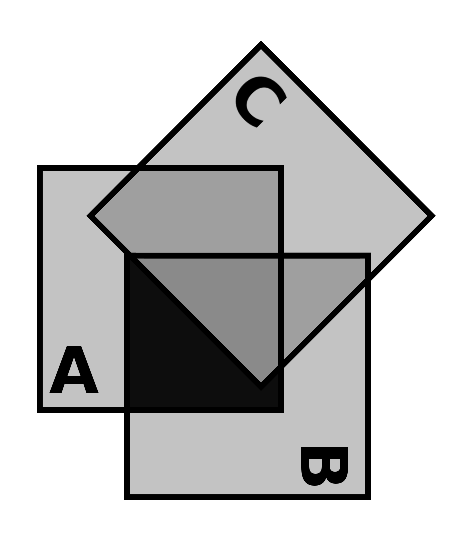
\includegraphics[width=\nPolarizerWidth]{pictures/polarizers.eps}
		}}
	\end{minipage}
}
	
\end{tabular}

% Reference: REFLECTION OF LIGHT FROM DIELECTRIC AND CONDUCTOR
%            https://lecdem.physics.umd.edu/m/m7/m7-17.html
\item Reflections from an electrical insulator are polarized. Conductive reflectors do not polarize EMR.

% from Doug Welch, and extended by internet descriptions.
\item Light from a rainbow is polarized due to the reflection inside the water droplets.

\item Moonlight is slightly polarized. Rotating a polarized sunglass lens causes the moonlight to dim and brighten slightly.

\end{itemize}

}
}}
		}

		\rput[bl](9.5,0){
			\white\psset{cornersize=absolute,linearc=4pt,fillstyle=solid,fillcolor=Black, linecolor=white}\psframebox{\parbox[t][3.8in]{3.2in}{%Refraction
{
\psset{linestyle=none}
\textcolor{white}{\Large Refraction}

%Prism
\begin{itemize}
\item%
\begin{tabular}[t]{@{}l@{\hspace{0.1in}}l}%
	\begin{minipage}[t]{1.5in}\textcolor{white}{%
		Refraction, or bending of EMR, is dependent on wavelength. All wavelengths of EMR can be refracted by using the proper materials.
		White light can be spread by refraction into a spectrum of its composite colors with a glass prism.	
	% 	A right-angle prism will act as a mirror instead of a light refractor.  The critical angle of a true light-refracting prism is 42\degree.
		}%
	\end{minipage}&
	\raisebox{-0.9in}{\begin{minipage}[t]{1.42in}{%
			\setlength{\fboxsep}{0pt}%
			\setlength{\fboxrule}{0.5pt}%
			\fbox{
\includegraphics[scale=0.8]{pictures/prism.eps}}%
			}%
		\rput[b](-.75in,-.16in){\textcolor{white}{\footnotesize\ Glass prism}}
		%\begin{center}Glass prism\end{center}
	\end{minipage}}
\end{tabular}

\item%
\begin{tabular}[t]{@{}l@{\hspace{0.1in}}l}%
	\begin{minipage}[t]{1.35in}{%
		Convex and concave lenses make objects appear closer and further and are used to correct far-sightedness and near-sightedness.
	}%
	\end{minipage}&
 	\raisebox{0.1in}
	{\begin{minipage}[t]{1.11in}%
		\rput(0.33,-.3){
			%Convex
			\psframebox{
				\psscalebox{0.9}{
					\psset{linestyle=solid,fillstyle=solid,fillcolor=darkgray}
					\psarc{c-c}(+.693,0){.8}{150}{210}
					\psarc{c-c}(-.693,0){.8}{330}{30}
					\psset{linestyle=solid,fillstyle=none}
					\psline{}(-.4,+.207)(-0.08,+.207)(.086,+.180)(.4,-.1)
					\psline(-.4,-.207)(-0.08,-.207)(.086,-.180)(.4,+.1)
				}
				\rput(0,-.4){\white Convex}
% 				\rput(0,-.47){\white lens}
			}
			%Concave
			\rput(0.68,0){
				\psframebox{
					\psscalebox{0.9}{
						\psclip{\psframe[fillstyle=none,linestyle=none,linearc=0,framearc=0](-.165,-.4)(.165,.4)}
						\psframe[fillstyle=solid,fillcolor=darkgray,linestyle=none,linearc=0,framearc=0](-.15,-.4)(.15,.4)
						\psset{linestyle=solid,fillstyle=solid,fillcolor=Black}
						\pscircle(+.85,0){.8}
						\pscircle(-.85,0){.8}
						\psline(-.157,-.389)(+.157,-.389)
						\psline(-.157,+.389)(+.157,+.389)
						\endpsclip
						\psset{linestyle=solid,fillstyle=none}
						\psline(-.4,+.180)(-0.086,+.180)(.08,+.207)(.4,+.4)
						\psline(-.4,-.180)(-0.086,-.180)(.08,-.207)(.4,-.4)
					}
					\rput(0,-.4){\white Concave}
% 					\rput(0,-.47){\white lens}
				}
			}
		}
	\end{minipage}}
	\end{tabular}

\item%
\begin{tabular}[t]{@{}l@{\hspace{0.14in}}l}%
	\begin{minipage}[t]{1.48in}\textcolor{white}{%
		Heavy objects like dense galaxies, stars, and large planets cause light to bend due to gravitational lensing as seen here in galaxy cluster Abell 2218:
		}%
	\end{minipage}&
	\raisebox{0.00in}{%
		\begin{minipage}[t]{1.16in}
			%http://imgsrc.hubblesite.org/hu/db/2004/08/images/a/formats/large_web.jpg
			\rput[tl]{90}(0,-.9){\textcolor{gray}{\footnotesize STScI}}
			\rput[tl]{0}(0.1,0.15){%
			\setlength{\fboxsep}{0pt}%
			\setlength{\fboxrule}{0.5pt}%
			\fbox{\includegraphics[width=1.18in]{pictures/gravlens.eps}}%
			}%
		\end{minipage}
	}
\end{tabular}
	
\end{itemize}

}

%Gravity lens - manually drawn
%\psframebox{
%	\rput(-.75,0){
%		\PstStarFive[unit=.1,
%			fillstyle=solid,
%			fillcolor=white,
%			linestyle=solid,
%			linecolor=white,
%			PolyIntermediatePoint=0.3,
%			PolyRotation=45]
%	}
%	\pscircle[linestyle=solid,
%		linecolor=white,
%		fillstyle=solid,
%		fillcolor=Black](0,-.1){.2}
%	\pscurve[linestyle=solid,linecolor=white,fillstyle=none](-.6,.05)(0,+.15)(.6,.05)
%	\rput(.85,0){
%		\psclip{\psline[fillstyle=none,linestyle=solid,linecolor=white,linearc=0](.3;150)(0,0)(.3;210)}
%			\psclip{\pscircle[linestyle=solid,linecolor=white,fillstyle=solid,fillcolor=white]{.2}}% Eyeball
%			\rput(-.2,0){
%				\pscircle[fillstyle=solid,fillcolor=gray]{.10}% Iris
%				\pscircle[fillstyle=solid,fillcolor=Black]{.05}% Pupil
%			}
%			\endpsclip
%		\endpsclip
%	}
%}
}}
			}

		\rput[bl](12.9,0){
			\white\psset{cornersize=absolute,linearc=4pt,fillstyle=solid,fillcolor=Black, linecolor=white}\psframebox{\parbox[t][3.5in]{2.3in}{%Reflection
{
\psset{linestyle=solid}
\textcolor{white}{\Large Reflection}

\begin{itemize}
	\item Reflection of EMR is dependent on wavelength as demonstrated when visible light and radio waves bounce off objects that X-Rays would pass through. Microwaves, which have a large wavelength compared to visible light, will bounce off metal mesh in a microwave oven whereas visible light will pass through.
	
	%Mirror
	\rput(0.5\linewidth,-.6){%Reflection
{
\psset{linestyle=solid}
\textcolor{white}{\Large Reflection}

\begin{itemize}
	\item Reflection of EMR is dependent on wavelength as demonstrated when visible light and radio waves bounce off objects that X-Rays would pass through. Microwaves, which have a large wavelength compared to visible light, will bounce off metal mesh in a microwave oven whereas visible light will pass through.
	
	%Mirror
	\rput(0.5\linewidth,-.6){%Reflection
{
\psset{linestyle=solid}
\textcolor{white}{\Large Reflection}

\begin{itemize}
	\item Reflection of EMR is dependent on wavelength as demonstrated when visible light and radio waves bounce off objects that X-Rays would pass through. Microwaves, which have a large wavelength compared to visible light, will bounce off metal mesh in a microwave oven whereas visible light will pass through.
	
	%Mirror
	\rput(0.5\linewidth,-.6){\input{pictures/reflection.tex}}
	
	\vspace{0.72in}
	\item EMR of any wavelength can be reflected, however, the reflectivity of a material depends on many factors including the wavelength of the incident beam.

	\item The angle of incidence ($\theta_i$) and angle of reflection ($\theta_r$) are the same.

\end{itemize}


}
}
	
	\vspace{0.72in}
	\item EMR of any wavelength can be reflected, however, the reflectivity of a material depends on many factors including the wavelength of the incident beam.

	\item The angle of incidence ($\theta_i$) and angle of reflection ($\theta_r$) are the same.

\end{itemize}


}
}
	
	\vspace{0.72in}
	\item EMR of any wavelength can be reflected, however, the reflectivity of a material depends on many factors including the wavelength of the incident beam.

	\item The angle of incidence ($\theta_i$) and angle of reflection ($\theta_r$) are the same.

\end{itemize}


}
}}
		}

	}
	
	\rput[br](19.14,0.8){
		\white\psset{
			cornersize=absolute,linearc=4pt,fillstyle=solid,fillcolor=Black, linecolor=white}\psframebox{\parbox[t][3.2in]{3.5in}{
				{
{\Large {\bfseries I}nfrared {\bfseries R}adiation (IR)}
\begin{itemize}

\item IR is sensed by humans as heat and is below the range of human vision. All creatures emit IR, and snakes can detect it.

\item IR remote control signals are invisible to the human eye but can be detected by some electronic cameras.

\newlength{\nIRdogHeight}   \setlength{\nIRdogHeight}{0.88in}
\item
\begin{tabular}[t]{@{}ll@{\hspace{0.05in}}r}
\raisebox{-.43\nIRdogHeight}{
	\begin{minipage}{.73in}
		{
			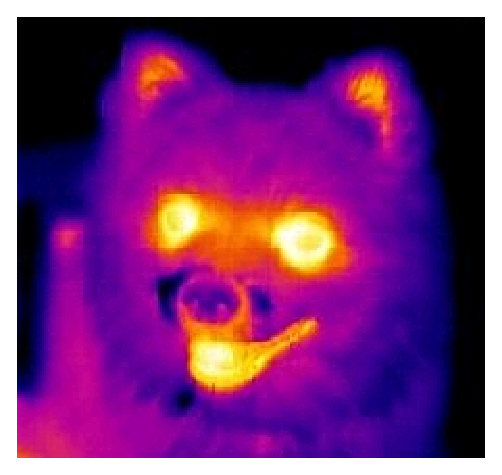
\includegraphics[height=\nIRdogHeight]{pictures/Infrared_dog.eps}
			\rput[b](-.4in,-.16in){\textcolor{gray}{\footnotesize\ NASA/IPAC}}
		}
	\end{minipage}
}&
 \begin{minipage}[t]{1.4in}Night vision scopes/goggles use a special camera that senses IR and converts the image to visible light. Some IR cameras employ an IR lamp to help illuminate the view.\end{minipage}&
 %
 % Get a regular outdoor night time photo with flash, use GIMP->Filters->EG-> Infrared Simulation
\raisebox{-.43\nIRdogHeight}{\
	\begin{minipage}{1in}
		{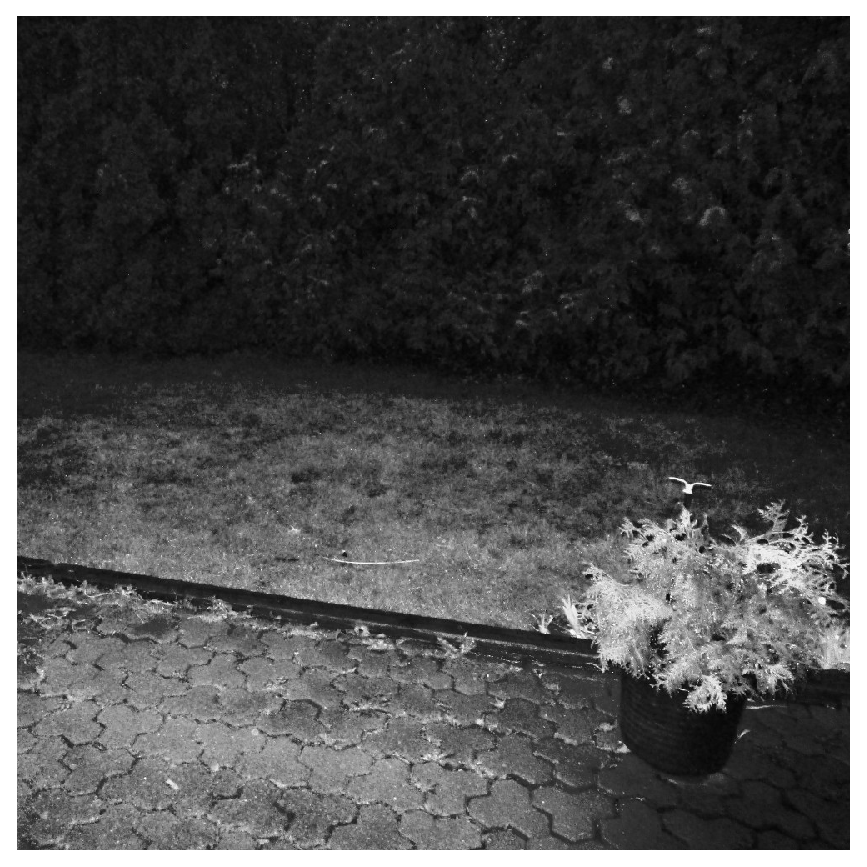
\includegraphics[height=\nIRdogHeight]{pictures/nightvision.eps}}
	\end{minipage}
}
\end{tabular}

\item A demonstration of IR is to hold a metal bowl in front of your face. The IR emitted by your body  will be reflected back using the parabolic shape of the bowl and you will feel the heat.

\item IR LASERs are used for cutting material.

%Information provided by Edward  Alan Dowdell:
%http://www.fiber-optics.info/fiber-history.htm
%http://www.thefoa.org/tech/wavelength.htm
%http://www.webopedia.com/TERM/E/EDFA.html
\item Fiber-optic based infrared communication signals are sometimes amplified with Erbium-Doped Fiber Amplifiers  \scalebox{.8}{\psframebox[linestyle=none]{\fiberoptics{0.13,-.13}{EDFA}}}
\end{itemize}
}

			}\
		}
	}
%
	%Company copyright 
	\rput[br](19.10,0.5){%
		\white\psset{
			cornersize=absolute,linearc=4pt,fillstyle=solid,fillcolor=Black,linecolor=white}\psframebox{\parbox[t][0.1in]{3.5in}
			{
				\renewcommand{\dateseparator}{}%No date separator required for version number,too confusing.
				\centering \copyright \hspace{0.1in} \url{unihedron.com}  \hspace{0.2in} \textcolor{gray}{\today}%
			}\
		}%
	}%
%
	%Crop marks to remove bleed
	{\psset{linecolor=yellow,linewidth=1pt}
		\multido{\iY=0+39}{2}{\psline(-0.4 ,\iY )(-.1,\iY )} %Left side
		\multido{\iY=0+39}{2}{\psline(20.1 ,\iY )(20.4,\iY )} %Right side
		\multido{\iX=0+20}{2}{\psline(\iX ,-0.4)(\iX ,-0.1)} %Bottom side
		\multido{\iX=0+20}{2}{\psline(\iX ,39.1)(\iX ,39.4)} %Top side
	}

	%Visible cropped window (comment out for production).
% 	\rput(0,0){\psframe[linecolor=white,linewidth=1pt](0,0)(20,39)}
  
	%Visible border window (comment out for production).
% 	\rput(0.5in,0.5in){\psframe[linestyle=dotted, linecolor=white,linewidth=1pt](0,0)(19,38)}

	%Comment this right-side sine-wave rainbow out for faster compiling/testing
	\rput[b](19.25in,-4.4in){%Rainbowwave.tex

%This feature uses a lot of LaTeX memory.
% As root:
%  edit the texmf.cnf 
%    and change main_memory = 12,435,456
% then run:
%   fmtutil-sys --all

% Description: Rainbow colored sine wave

% http://www.fon.hum.uva.nl/praat/manual/Script_for_creating_a_frequency_sweep.html
%formula M*sin(A*x+B*(x^2)/C)
%\nA = Start frequency
%\nB = End frequency-Start frequency
%\nC = number of samples
%\nM = multiplying height factor since we need smaller pgfplots height than allowed.
\newcommand{\nRainbowStartFreq}{5}% Start frequency.
\newcommand{\nB}{40}% End frequency - start frequency. (was 40, seems to make no difference)
\newcommand{\nC}{1e3}% Number of samples. (was 1e3)
\newcommand{\nM}{0.35}% Multiplying factor for amplitude.

\pgfplotsset{
	compat=1.14,
	axis line style={draw=none},
	tick style={draw=none},
	xticklabels=\empty,
	yticklabels=\empty,
	colormap={redblue}{
		rgb255(0cm)=(128,0,0); rgb255(1cm)=(255,0,0); rgb255(2cm)=(255,255,0);
		rgb255(3cm)=(100,255,0);rgb255(4cm)=(0,255,255); rgb255(5cm)=(0,0,180)},
	samples=8000,%was 1000, but capacity exceeded , looked into -shell escape external method make nonoverlapping pdfs (on separate pages).
	domain=1:\nC%range
}

\begin{tikzpicture}[rotate=90]
	\begin{axis}[width=46.1in,height=0.9in]%height was 48
		\addplot [white,line width=3pt,line join=round, line cap=round]             {\nM * sin(\nRainbowStartFreq * x + \nB * (x^2) / \nC)};
		\addplot [mesh,point meta=x,line width=2pt,line join=round, line cap=round] {\nM * sin(\nRainbowStartFreq * x + \nB * (x^2) / \nC)};
	\end{axis}
\end{tikzpicture}
}
	
\end{pspicture}%


\end{document} %===============================================================
